%% -*- fill-column:80; eval:(visual-line-mode 1);  eval:(auto-fill-mode 0)  -*-
\documentclass[12pt,letterpaper]{article}
 \setcounter{page}{0}

\usepackage{mathtools} 
\usepackage{bbm}
\usepackage[multiple]{footmisc}
\usepackage{floatpag,amsmath,amsthm,amssymb}
\newtheorem{proposition}{Proposition}
\numberwithin{equation}{section}
\newtheorem{nono-prop}{Proposition}[]

% Figure panel header font
\newcommand{\panel}{\fontfamily{phv}\selectfont\scriptsize\textbf}
\usepackage{amsmath} 
\DeclareMathOperator*{\argmin}{arg\,min}
\DeclareMathOperator*{\argmax}{arg\,max}

%%%%%%%%%%%%%%%%%%%%%%%%%%%%%%%
%% LOAD LOCAL COMPILATION PATHS
%%%%%%%%%%%%%%%%%%%%%%%%%%%%%%%

%% DON'T CHANGE ANY OF THESE PATHS. FOR LOCAL COMPILE, EDIT YOUR
%%                                            ~/include.tex ONLY
\newcommand{\HOME}{\string~}
\input{\HOME/include.tex}

% include standard package
\usepackage[latin1]{inputenc}
% \usepackage{lmodern} % keep or kill this??  might affect italics.
\usepackage{setspace}
\usepackage{amsmath}
\usepackage{amsthm}
\usepackage{amsfonts}
\usepackage{longtable}
\addtolength{\textwidth}{5cm}
\addtolength{\textheight}{5cm}
\usepackage{fullpage}
\usepackage{amssymb}
\usepackage[colorlinks=true]{hyperref}
\usepackage{url}
\usepackage{graphicx}
\usepackage{epstopdf}
\usepackage{multirow}
\usepackage{array}
\usepackage{harvard}
\usepackage{tabularx}
\citationmode{abbr}

\usepackage{float}
% \usepackage{perpage}
% \MakeSorted{figure}
% \MakeSorted{table}
\usepackage{lscape}
\usepackage{verbatim}
\usepackage{pdflscape}
\usepackage{chngcntr}
\usepackage{appendix}
\usepackage{booktabs,calc}
\usepackage{ulem}

% allow yellow highlighting in tables
\usepackage{color,colortbl}
\usepackage{soul}
\definecolor{Yellow}{rgb}{.88,1,.65}
\definecolor{Green}{rgb}{.65,1,.65}
\definecolor{Red}{rgb}{1,.65,.65}

\citationstyle{dcu}

\usepackage[labelfont=bf,center,large,labelsep=newline]{caption}
\usepackage{subfig}
% \counterwithout{subtable}{table}
\def\changemargin#1#2{\list{}{\rightmargin#2\leftmargin#1}\item[]}
\let\endchangemargin=\endlist

% define subscript / superscript commands
\newcommand{\superscript}[1]{\ensuremath{^{\textrm{#1}}}}
\newcommand{\subscript}[1]{\ensuremath{_{\textrm{#1}}}}

% create a shortcut for newlines in captions:
\newcommand{\cnewline}{\hspace{\linewidth}}

%format paper to save trees
\usepackage[right=1in,left=1in,top=1in,bottom=1in]{geometry}
\usepackage{savetrees}

%AER style headers
\def\thesection{\arabic{section}}
\def\thesubsection {\thesection.\arabic{subsection}}

% set home path
\newcommand{\HOME}{\string~}

\usepackage{geometry} 
\usepackage{fancyhdr} 

\pagestyle{fancy}
\fancyhead[RE,RO]{}
\fancyhead[LE,LO]{}
\markright{} 
\lhead{}
\chead{}
\rhead{\thepage}
\cfoot{} % get rid of the page number 
%\fancyheadoffset[loh,reh]{-in}
\renewcommand{\headrulewidth}{0pt}
\renewcommand{\footrulewidth}{0pt}
\setlength{\headheight}{15pt}

% \setlength{\headsep}{24pt}

% package for color-shared tables
\usepackage[table]{xcolor}

% disable hyperlinks, which were breaking on appendix references
\usepackage[options]{nohyperref}

\title{Intergenerational Mobility in India: \\ New Measures and
  Estimates Across Time and Social Groups\footnote{We are
    thankful for useful discussions with Alberto Abadie, David Autor,
    Emily Blanchard, Raj Chetty, Eric Edmonds, Shahe Emran, Francisco
    Ferreira, Amy Finkelstein, Nate Hilger, Larry Katz, David Laibson, Ethan Ligon,
    Erzo Luttmer, Whitney Newey, Elias Papaioannou, Nina Pavcnik,
    Bruce Sacerdote, Frank Schilbach, Na'ama Shenhav, Forhad Shilpi, Andrei Shleifer,
    Gary Solon, Bob Staiger, Doug Staiger, Chris Snyder and Elie
    Tamer, among others. Annaka Balch, Ali Campion, Toby Lunt, Ryu
    Matsuura, and Taewan Roh provided excellent research
    assistance. This project received financial support from the IZA
    GLM-LIC program. This material is based upon work supported by the National Science Foundation Graduate Research Fellowship under Grant No. 1122374. This paper
    contains some material previously contained in the retired paper, ``Getting Signal
    from Interval Data: Theory and Applications to Mortality and
    Intergenerational Mobility.'' An earlier version of this paper had the subtitle ``Across Time, Space, and Communities.''}} \author{Sam Asher\thanks{Imperial College London, sam.asher@imperial.ac.uk} \\ \\ Paul
  Novosad\thanks{Dartmouth College, paul.novosad@dartmouth.edu,
    corresponding author} \\ \\ Charlie Rafkin\thanks{Massachusetts Institute of Technology,
    crafkin@mit.edu} \\ \\ }

%%%%%%%%%%%%%%%%%%%%%% 
% TITLE PAGE
%%%%%%%%%%%%%%%%%%%%%% 
\begin{document}
% \newgeometry{left=1.25in,right=1.25in,bottom=1.25in,top=1.25in}

\date{September 2022}
\maketitle
% JEL CODES J62 (intergenerational mobility) O15 (human
% development/income distribution) I24 (education and inequality)
% C14 (nonparametric methods)

\begin{abstract}
\thispagestyle{empty}
  We study intergenerational mobility in India.  We propose a new measure of upward mobility: the expected education rank of a child born to parents in the bottom half of the education distribution. This measure works well under data constraints common in developing countries and historical contexts. Intergenerational mobility in India has been constant and low since before liberalization. Among sons, we observe rising mobility for Scheduled Castes and declining mobility among Muslims. Daughters' intergenerational mobility is lower than sons', with less cross-group variation over time. A natural experiment suggests that affirmative action for Scheduled Castes has substantially improved their mobility.

\end{abstract}
\newpage
\clearpage
\setcounter{pag}{1}
\spacing{1.5}
\section{Introduction}
\label{sec:intro}

% cite for acknowledgements
\nocite{bratberg2017}

There are two widely held narratives regarding access to opportunity in India. On the one hand, economic liberalization, rapid economic growth, and urbanization have vastly expanded the set of opportunities available to Indians, leading to the emergence of a large middle class. The political sphere has also opened, with the growth of a wide range of parties organized around caste, region, and ideology. Decades of affirmative action programs have targeted government benefits at historically disadvantaged groups. On the other hand, some of India's entrenched inequalities seem as persistent as ever. Marriage across religious, caste, and class lines is exceedingly rare. Elites in business, government and civil society are still largely from the upper classes and castes. Inequality has risen, and religious cleavages may be deepening \cite{chancel2019}. In this paper, we shed light on changing access to opportunity in India by studying the intergenerational transmission of economic status \cite{solon1999,black2011,chetty2014c,chetty2018}, with a particular emphasis on the 478 million people (39\%) who belong to India's major disadvantaged groups (Muslims, Scheduled Castes, and Scheduled Tribes).

We seek to measure the persistence of socioeconomic \textit{rank} across generations, isolating intergenerational mobility from changes in inequality and growth, in the spirit of \citeasnoun{solon1999}. Recent advances in the literature on intergenerational mobility have yielded a set of measures based on the conditional expectation function of a child's socioeconomic rank, given a parent's rank (henceforth, the CEF); the most notable of these is \textit{absolute upward mobility}, which is the income rank of a child born to a parent at the 25th percentile \cite{chetty2014c}. These measures have several desirable features, two of which we highlight: (i) by focusing on ranks, they isolate mobility from economic growth and inequality, which is crucial in a rapidly-growing country like India; (ii) they are directly interpretable as mobility estimators for population subgroups, like Scheduled Castes.\footnote{Section \ref{sec:method} explains why the earlier canonical class of linear estimators, such as the regression coefficient from a regression of child education on parent education, are difficult to interpret for population subgroups.}

We cannot apply these existing measures to study intergenerational mobility in India. Linked parent-child income data is unavailable in India, as in many developing countries. If it were available, it would be difficult to interpret in multigenerational households with joint production. For these reasons, studies on intergenerational mobility in developing countries and historical contexts have often used education as the primary measure of social status.\footnote{Intergenerational educational mobility is also directly of interest; canonical intergenerational mobility models like \citeasnoun{loury1981}, \citeasnoun{becker1986}, and \citeasnoun{galor1993} often emphasize the role of human capital investment. Recent studies of intergenerational mobility focusing on education include \citeasnoun{black2003}, \citeasnoun{guell2013}, \citeasnoun{wantchekon2015a}, \citeasnoun{card2022}, \citeasnoun{alesina2018}, and \citeasnoun{eshaghnia2022}. More are summarized in \citeasnoun{black2011}.} We highlight and then resolve a key challenge that arises in the use of CEF-based mobility estimators with education data: education is reported in bins --- often very large bins. Among parents of the 1950--1969 generations in India, more than 50\% of fathers (and 80\% of mothers) have bottom-coded levels of education; identifying a parent at the 25th percentile (or any other) is fraught, and naive approaches can produce incorrect results.

We gain traction on this problem by recasting it as an interval censoring problem, such that the binned education data reflect a continuous (but unobserved) latent rank distribution.\footnote{Section~\ref{ssec:math} discusses this assumption in detail and sketches out how it arises directly from a standard human capital model.} This framing of the problem lets us draw on tools from the partial identification literature to put bounds on the parent-child rank CEF \cite{manski2002,nra2020mort}. We introduce a new measure of upward mobility, \textit{bottom half mobility}, which is the expected rank of a child born to a parent in the bottom half of the education distribution. Bottom half mobility has a very similar interpretation to absolute upward mobility, but it can be bounded tightly even in contexts with severe interval censoring. Our approach further reveals that, once interval censoring is taken into account, other canonical measures like absolute upward mobility and the rank-rank gradient have bounds that are too wide to be meaningful.\footnote{Naive application of these tools that ignoring the censoring problem leads to results that are misleadingly precise, because they ignore the loss of information associated with the coarse measurement of education; they may also be biased (see Section~\ref{sec:results}).}

To study upward mobility in India, we use data from the 2012 India Human Development Survey (IHDS). A key feature of this dataset is that individuals were asked about their parents' education level. We thus observe parent-child links even when parents and children live in different households, and we can measure changes in mobility using older cohorts. We document trends in educational mobility from the 1950--59 to the 1985--89 birth cohorts. We focus on measuring mobility from fathers to sons and daughters; mobility from mothers to children cannot be bounded tightly because the bottom-coding of mothers' education is so severe.

We present two main results. First, upward mobility has remained constant over the entire sample period, despite dramatic gains in average levels of education and income. An Indian son born in the bottom half of the parent education distribution in 1985--89 (our youngest cohort) can expect to obtain percentile 37.7; a daughter obtains percentile 35.6.\footnote{We compute educational attainment ranks for sons and daughters separately because men and women mostly compete in separate labor markets and education plays a different role in determining their life outcomes.} A similar child in the U.S., which has low intergenerational mobility by OECD standards, on average attains education percentile 41.7.\footnote{In a society where children's outcomes are independent of parents (i.e. perfect mobility), a child born in the bottom half of the distribution obtains the 50th percentile on average. In a society with no upward mobility, i.e. where all children obtain the same percentile as their parents, the same child attains the 25th percentile.} This suggests that India's decades of economic growth have lifted the living standards of individuals in the bottom half of the socioeconomic distribution without substantially changing their likelihood of moving to a higher socioeconomic \textit{rank}. By contrast, a naive application of the canonical rank-rank gradient estimator to our data would suggest that mobility had improved significantly.

Second, we show that upward mobility has changed substantially over time for some social groups, particularly among sons. We divide the population into Scheduled Castes (SCs), Scheduled Tribes (STs), Muslims, and Forwards/Others. Consistent with prior work \cite{hnatkovska2012,emran2015}, we find that sons from India's constitutionally protected marginalized groups, the Scheduled Castes and Tribes, have closed respectively 50\% and 30\% of the mobility gap with Forwards/Others. In contrast, upward mobility for Muslim sons has steadily declined from the 1960s to the present. The expected educational rank of a Muslim man born in the bottom half of the parent distribution has fallen from between percentiles 31 and 34 to a dismal 29.\footnote{The comparable figure for U.S. Black men is 35.} Muslim sons have considerably worse upward mobility today than both Scheduled Castes (38) and Scheduled Tribes (33), a striking finding given that, compared to Muslims, STs tend to live in more rural and remote areas. Higher caste groups have experienced constant and high upward mobility over time, a result that contradicts a popular notion that it is increasingly difficult for higher-caste Hindus to get ahead.\footnote{The sample size of the IHDS is too small to study geographic variation in any detail. For a preliminary analysis of the micro-geographic variation in upward mobility using individuals aged 20--23 in the high resolution 2011--12 Socioeconomic and Caste Census (SECC), please see the working version of this paper \cite{anr2019mob}.}

Our measures for father-daughter mobility are less precise, but the subgroup patterns appear to be different. Daughters from poor Muslim, SC, and ST households all have persistently lower mobility than Forwards/Others. There is minimal convergence over the sample period; the bounds on changes are consistent with women's mobility being either stable or declining slightly.

The final section of the paper examines several mechanisms for the divergence of Scheduled Castes from Muslims over the last 30 years. We show that this divergence cannot be explained by differential returns to education, occupational patterns, geography, or differential fertility. However, we find suggestive evidence that the basket of affirmative action policies targeted to India's scheduled groups (but not to Muslims) has played a key role in their rising mobility. Following \citeasnoun{cassan2017}, we study a natural experiment that added many castes to the Scheduled Caste lists in 1977 following a rules-based mechanism. We show that caste groups that were newly assigned to Scheduled Caste status on average experienced a 7--8 rank point increase in upward mobility over the next twenty years. This is the same size as the rank mobility gap that has opened between Muslims and Scheduled Castes over the same period. Our findings are thus consistent with the possibility that educational quotas, government job reservations, and other affirmative action policies are fully responsible for the upward mobility gap that has opened between Scheduled Castes and Muslims. However, because we are limited to birth cohort $\times$ demographic group variation and only a small sample of individuals whose SC status changed (N=696), these results are suggestive and not dispositive. 

This paper makes both methodological and empirical contributions. Methodologically, we show how to calculate CEF-based mobility measures using education data; our proposed measure, bottom half mobility, may be useful in many contexts beyond India. To our knowledge, the bias caused by ignoring interval censoring in education data has not been recognized by prior work on intergenerational educational mobility. We describe the relationship between our measure and others in the literature in Section~\ref{sec:comparison}.

Empirically, we present several previously unknown facts about upward mobility
in India. Our findings imply that virtually all of the upward mobility gains in India over recent decades have accrued to Scheduled Castes and Tribes, groups that have constitutional protections, reservations in politics and education, and who have been specifically targeted by development policies. There is no evidence that any of these gains have come at the expense of higher-caste groups. On the other hand, mobility has declined for Muslims. We are not aware of studies of intergenerational mobility for Indian Muslims, even though they number almost 200 million people (even higher than the number of people in Scheduled Castes).\footnote{Other economics papers on Indian Muslims include \citeasnoun{khamis2012} and \citeasnoun{bhalotra2010}, who note poor education outcomes among Muslims. The Sachar Committee Report \citeyear{sachar2006} and \citeasnoun{basant2010} summarize some recent research on Muslims on India, none of which addresses intergenerational mobility.}

Our analysis of bottom half mobility has several limitations. First, by averaging results in the bottom half of the distribution, bottom half mobility may conceal changes within the bottom half. We cannot rule out the possibility that outcomes for the bottom 10\% have improved substantially, while, for example, outcomes for percentiles 40 through 50 have declined.\footnote{Testing for changes within the bottom half requires different data on parents, since the coarse education bins in the data mean that information on relative parent status cannot be inferred from parent education.} Going forward, we use the terms ``upward mobility'' and ``bottom half mobility'' interchangeably; but our results are by no means conclusive about upward mobility from the very bottom of the distribution.

Second, in principle, the observed divergence between SCs and Muslims could mechanically arise if Muslim parents are increasingly concentrated among the lowest latent ranks in the bottom half (which we would not observe directly). We present a host of tests that reject such an explanation; similar tests would be advised when using our method to study population subgroups in other contexts.

Our estimates contribute to a growing literature on intergenerational mobility.\footnote{For review papers on intergenerational mobility, see \citeasnoun{corak2013a}, \citeasnoun{black2011}, and \citeasnoun{roemer2016}. Recent work on intergenerational mobility has described the United States \cite{chetty2014b,chetty2014c,chetty2018}, western Europe \cite{bratberg2017}, and Africa \cite{alesina2018}, among many other regions.} Post-independence India is an important setting for studying upward mobility, both because it has undergone rapid economic change, and because of the history of the caste system, which has been thought to entrench mobility across generations. Our finding that India's growth episode had little effect on rank mobility recalls other recent studies that have found intergenerational persistence in the context of substantial social upheaval \cite{ager2021,alesina2020b}. Prior work on India has: (i) emphasized absolute outcomes (such as consumption), which are rising for all groups due to India's substantial economic growth \cite{maitra2009,hnatkovska2013}; or (ii) compared subgroups using the parent-child outcome correlation or regression coefficient, which describes the outcomes of subgroup members relative to their own group, rather than to the national population \cite{hnatkovska2013,emran2015,azam2015}.\footnote{Note that there is a parallel literature examining the persistence of income within an individual lifetime in India; this is sometimes described as \textit{income} or \textit{economic mobility}. That literature is focused largely on measurement error in income over the course of an individual's lifetime and is thus not directly related to our work \cite{azam2016,li2019}.} Studies of affirmative action in India have found impacts on educational attainment of SC/STs \cite{frisancho2012,bagde2016,cassan2017,khanna2020}, but have not examined intergenerational mobility.

More broadly, our paper relates to research on religion and economic development  \cite{mccleary2006,becker2009}. \citeasnoun{alesina2020} and \citeasnoun{platas2018} find low mobility and educational outcomes for Muslims in Sub-Saharan Africa, where Islam plays a different cultural, political and social role from in India.\footnote{See also \citeasnoun{kuran2018} for a summary of the literature on Islam and economic performance.}

Stata code to calculate our mobility measures and replicate this paper is posted online.\footnote{\url{https://github.com/devdatalab/paper-anr-mobility-india/}} 

\section{Context on Intergenerational Mobility in India}
\label{sec:context}

India's rapid economic growth and pervasive caste system make it a particularly
important setting for understanding intergenerational mobility for at least two reasons. First, Indian society has undergone a large transformation over the last forty
years. Economic liberalization, starting in the 1980s, dismantled many parts of
India's post-independence experiment with central planning. Decades of sustained
economic growth have resulted in substantial reductions in poverty and the rise of a
large middle class. This setting thus lets us examine
intergenerational mobility in the context of rapid economic growth in a
large developing nation. 

Second, India's caste system is characterized by a set of informal rules that inhibit intergenerational mobility by preventing individuals from taking up work outside of their caste's traditional occupation and from marrying outside of their caste. While some have argued that economic growth is reducing the influence of old social and economic divisions, caste and religion remain important predictors of economic status \cite{munshi2006,ito2009,hnatkovska2013,shariq2019}. Since independence in 1947, the government has systematically implemented policies intended to reduce the disadvantage of communities that are classified as Scheduled Castes or Scheduled Tribes. These groups are targeted by a range of government programs and benefit from reservations in educational and political institutions.

India's Muslims constitute a similar population share as the Scheduled Castes
and Scheduled Tribes (14\% for Muslims vs. 17\% for SCs and 14\% for STs). While
Muslim disadvantage has been widely noted, including by the well-known federal
Sachar Report \citeyear{sachar2006}, there are few policies in place to protect
them and there has not been an effective political mobilization in their
interest. To the contrary, a large-scale social movement (the Rashtriya
Swayamsevak Sangh, or RSS) and several major political parties have rallied
around pro-Hindu platforms and policies which arguably discriminate against
Muslim religious, economic, and cultural practices. Violent anti-Muslim riots
have been closely tied to political parties and political movements
\cite{wilkinson2006v,berenschot2012,blakeslee2018}.

\section{Methods: Measuring Intergenerational Mobility in Developing Countries}
\label{sec:method}

Our goal is to study the persistence of socioeconomic rank across generations, holding constant changes in inequality and growth, following the notion of intergenerational mobility in \citeasnoun{solon1999} and \citeasnoun{chetty2014b}. India's rapid growth and changes in inequality have been widely studied.\footnote{See, for example, \citeasnoun{rodrik2005}, \citeasnoun{lamba2020}, and \citeasnoun{chancel2019}.}  Our goal is to understand whether India's major growth episode has affected individuals' ability to move up in the \textit{relative} status distribution.

Like many other studies in developing countries and historical settings we focus on education as the primary measure of relative social status \cite{solon1999,guell2013,wantchekon2015a,card2022,derenoncourt2022,alesina2018}. Income mobility is difficult to measure in these settings for three reasons. First, high quality linked parent-child income data are rare. Second, measurement error in income (which is substantial) leads mobility estimates to be biased downward; education levels are measured more accurately and do not vary over the life cycle. Third, earnings are difficult to ascribe to individuals in multigenerational households with joint production. In addition to these measurement concerns, human capital investment is a key form of intergenerational investment, and plausibly a target of public policy. Thus, intergenerational educational mobility is important even when income is observed.

\subsection{Rank CEF-Based Mobility Measures and Intergenerational Educational Mobility}
\label{sec:method_bg}

Our paper builds on the seminal work of \citeasnoun{chetty2014b}, which proposed absolute upward mobility and other rank-rank CEF-based mobility measures. Absolute upward mobility (denoted as $p_{25}$ below) is the income rank of a child born to a parent at the 25th percentile \cite{chetty2014c}. This measure has several characteristics that make it desirable as a measure of upward mobility.

First, rank measures like $p_{25}$ distinguish mobility from economic growth and inequality. The canonical mobility estimator, the coefficient from a regression of child income on parent income (or the equivalent with education), combines information from changes in rank mobility and in inequality \cite{chetty2014b}. Similarly, the probability that a child obtains a higher raw socioeconomic outcome than their parent (used in \citeasnoun{chetty2016} and \citeasnoun{alesina2018}) simultaneously captures intergenerational mobility and economic growth. Indeed, in developing countries like India, most children obtain more income and education than their parents; but this in itself does not tell us whether children from the bottom have better access to the best opportunities than they did before.

% PN: last sentence needs improvement

Second, measures like $p_{25}$ are easily and meaningfully calculated for population subgroups. Comparing the class of linear mobility estimators (like the rank-rank gradient) across subgroups is less straightforward, because the gradient compares children's outcomes against more advantaged members only of their own group. Meaningful comparison thus requires examining both the subgroup gradient and the average outcome difference across groups \cite{hertz2008a,jacome2021}. In contrast, $p_{25}$ has the same interpretation for a subgroup as for the full population: it describes the expected rank of a child in the subgroup who is born to a parent at the 25th population percentile.\footnote{Indeed, we are not aware of any studies that have applied the \citeasnoun{hertz2008a} method to study educational mobility; \citeasnoun{jacome2021} is a particularly clear implementation using this method to study intergenerational income mobility in the U.S.} 

Last, $p_{25}$ directly describes outcomes in the bottom half of the distribution. The gradient class of mobility estimators assume linearity, but in fact linear rank-rank CEFs (as found in the United States) appear to be the exception rather than the rule.\footnote{The rank-rank CEF is highly linear in the United States, but non-linear CEFs are found in Canada, Europe, and as we show below, in India \cite{bratsberg2007,boserup2014,bratberg2017,connolly2019}.} 

The key challenge to estimating $p_{25}$ in education data is in defining what it means for a parent to be at the 25th percentile, when the 25th percentile appears in the middle of a coarse education bin. Figure~\ref{fig:moments_only}A demonstrates why this is difficult; the figure shows the average child education rank in each parent education rank bin for the 1960--69 and 1985--89 birth cohorts in India. In the 1960--69 birth cohort, 57\% of fathers report a bottom-coded education level; in the 1985--89 cohort, the figure is 36\%. How does one identify the expected child rank given a parent at the 25th percentile in these birth cohorts?\footnote{The graph makes clear that $p_{25}$ \textit{cannot} be proxied by the expected child rank in the parent bin containing the 25th percentile. When there is less censoring, the bottom bin represents a lower average set of parent ranks.}

Figure~\ref{fig:moments_only}B shows two conditional expectation functions that are both perfectly consistent with the 1960--69 moments. The data available cannot distinguish between these two functions, but they have different implications for upward mobility: one function implies a much higher expected rank for a child born to parents at the bottom of the distribution than the other. This example highlights our methodological insight: the CEF of child rank given parent rank can at best be partially identified from education data.

Coarse data like that described here is ubiquitous in the mobility literature. In developing countries, bottom-coding rates in excess of 50\% are widespread \cite{narayan2018}; the same is true for older generations in richer countries \cite{long2013}. Internationally comparable censuses often report education in as few as four categories.\footnote{Income mobility is also often based on censored estimates; in the well-known British Cohort Study, one income bin contains more than 30\% of the data.} Transforming transition matrices based on education or occupation data (with arbitrary coarse rank boundaries) into quantile transition matrices faces the same barriers as point-estimating the CEF above.

\subsection{Estimating Bounds on a CEF with Censored Education Data}
\label{ssec:math}

This subsection describes how we partially identify CEF-based mobility measures with coarse education data. The intuition behind our method is suggested by Figure~\ref{fig:moments_only}B. There are many possible CEFs that can fit the parent-child rank moments. The mobility measures we consider are functions of CEFs. Thus, for any given mobility measure, the bounds on the mobility measure are governed by the CEFs that minimize and maximize the measure, as long as the CEFs are consistent with the observed data. The method extends \citeasnoun{manski2002} and is derived in \citeasnoun{nra2020mort}. Appendix~\ref{app:formal_model} formalizes the bounds and reproduces the derivation for the case of upward mobility. This section focuses on an intuitive understanding of how the function is bounded.

We require only two assumptions to meaningfully bound the CEF. The first is definitional and already implicit in the discussion above: we assume the existence of a continuous, latent education rank. This assumption falls directly out of the standard human capital model. The latent education rank is based on the education level that would be chosen from a \textit{continuous} rather than a discrete set of education choices, if continuous choices were available. In practice, the educational choice set is lumpy, so we observe the rank only in coarse bins. The latent rank reflects how much the marginal benefit or cost of obtaining the next level of education (e.g., middle school) would need to change in order for a given individual to progress to that level. Individuals who would need only a small benefit shift to choose the next education level have the highest educational ranks within their rank bin. The latent rank is a proxy for the underlying factors that shift individuals' demand for education, which can be expected to be correlated with socioeconomic status \cite{Card1999}.\footnote{Like other papers on intergenerational educational mobility, we use education strictly as a proxy for socioeconomic status. Our interpretation is meaningful even if individuals at different latent ranks within the same bin have obtained \textit{exactly} the same number of years or hours of education. All else equal and in expectation, individuals with higher latent ranks will have socioeconomic advantages in dimensions other than years of education.}\superscript{,}\footnote{Transforming education levels into ranks is analogous to transforming individual incomes into ranks, which is ubiquitous in the mobility literature even when incomes are interval-censored \cite{rosenbaum2000}.}

Second, we assume that the conditional expectation of child education rank given parent education rank is monotonically increasing, including within education groups (where it is unobserved): having a more advantaged parent cannot make a child worse off. This assumption is motivated by the fact that average socioeconomic outcomes of children are strongly monotonic in parent socioeconomic outcomes across many socioeconomic measures and countries (Dardanoni et al., 2012), as well as in every birth cohort that we study in India (Appendix Table~\ref{tab:trans_matrices}).\footnote{In small samples, empirical non-monotonicity may emerge from monotonic distributions due to sampling error. This occurs at the very top of the distribution in a minority of subgroup-cohorts in our data; these non-monotonicities do not affect our calculations of upward mobility, which only use information from bins adjacent to the bottom half of the parent distribution.} The monotonicity assumption is not necessary; Appendix~\ref{app:formal_model} shows how other parametric assumptions can be used to bound the mobility function (e.g., constraining the maximum curvature of the underlying conditional expectation function). 

For parsimony, our framework considers a setting in which only the parent rank is interval-censored --- i.e., we take the child rank variable as \textit{not} censored. We address extensions with censored child ranks and potential bias from our approach in Section \ref{sec:childcens}.

With just these two assumptions, we can obtain sharp bounds on the CEF. Figure~\ref{fig:moments_only}C shows the bounds on the Indian CEF for the 1960--69 and the 1985--89 birth cohorts. The bounds will be tightest when parent education bins are small and the slope of the CEF is small --- when the two neighbhoring bins have moments that are close in magnitude, the monotonicity restriction constrains the CEF substantially. At the bottom of the education distribution, where the bins are large and the lowest values of the CEF are constrained only by the lower rank limit of zero, the bounds on the CEF are very wide. Intuitively, because of the censoring problem, there is simply not enough information the parent-child education distribution to bounds the child rank CEF at very low parent ranks.\footnote{Alternate estimation approaches might yield tighter predictions at the bottom of the distribution, but they do so only by imposing strong assumptions on the CEF. For example, if we estimate a linear rank-rank gradient, we can obtain a tight predicted value of the CEF at the bottom of the distribution. But the precision is misleading: the available data does not strongly motivate the linearity assumption that buys this precision.}

\textbf{Bottom half mobility.} We propose a measure, \textit{bottom half mobility}, which describes the expected outcome of a child born to parents in the bottom half of the parent distribution, or $\mu_0^{50} = E(y|x \in [0, 50])$ for child rank $y$ and parent rank $x$. Note the similarity in interpretation to absolute upward mobility, which is the expected outcome of a child born to the \textit{median} parent in the bottom half of the parent distribution, $p_{25}=E(y|x = 25)$.\footnote{If the CEF is linear, $p_{25}=\mu_0^{50}$; if the CEF is concave at the bottom of the parent distribution, then $\mu_0^{50} < p_{25}$. Most CEFs in the literature are concave, so $\mu_0^{50}$ effectively puts more weight on outcomes at the very bottom of the parent distribution than $p_{25}$.}\superscript{,}\footnote{Our framework can bound many other measures, such as $\mu_0^{20}$ (the expected rank of a child born in the bottom 20\%), $E(y > 80 | x < 20)$ (the probability that a child born in the bottom 20\% makes it into the top 20\%), or the conditional \textit{median} function of child rank given parent rank.} The measures $p_{25}$ and $\mu_0^{50}$ both describe the outcomes for groups in the bottom half of the socioeconomic distribution. In both cases, a value of 50 implies convergence to the mean rank in one generation, and a value of 25 implies no convergence at all. Both measures are useful, just as the mean and median of a given distribution have advantages and disadvantages as summary statistics. The main advantage of $\mu_0^{50}$ is that, as we show below, it can be tightly bounded in contexts where $p_{25}$ cannot.\footnote{Appendix~\ref{app:formal_model} provides a formal statement of analytical bounds on $\mu_a^b$ (derived in \citeasnoun{nra2020mort} for the estimation of individual mortality risk given the same individual's education rank). It shows how we estimate arbitrary functions of the CEF, including the best linear approximator to the CEF (i.e. the rank-rank gradient).} 

Figure~\ref{fig:mu_annotation} provides a graphical example that walks through the calculation of $\mu_0^{50}$ for the 1960--69 birth cohort in India. For an intuition on why $\mu_0^{50}$ is tightly bounded, consider the fact that the value of the CEF can in fact be point-estimated withing ranges that correspond to bin boundaries in the data. If a given parent education bin has rank boundaries $a$ and $b$, then $\mu_a^b$ is precisely equal to the expected child outcome in that rank bin. If we then seek to obtain a value that is \textit{close} that one, e.g. $\mu_a^{b+c}$ where $c$ is small, it will also be bounded tightly, because that new value is just a weighted mean of $\mu_a^b$ (which is point-estimated) and $\mu_b^{b+c}$, which has a small weight. In contrast, absolute mobility $p_i = E(y|x=i)$ cannot be point-estimated at any point on the CEF. The bounds on $\mu_a^b$ will thus be tightest when $a$ and $b$ are close to actual rank bin boundaries and when the slope of the CEF is small.

\subsection{Comparison with Other Measures of Educational Mobility}
\label{sec:comparison}

This subsection compares bottom half mobility to other measures of intergenerational educational mobility. First, \citeasnoun{alesina2018} study upward mobility across all of Africa and define upward mobility as the probability that a child born to a parent who has not completed primary school manages to do so. Their measure importantly captures whether poor countries now provide a minimal standard of education to households that have not been reached by the education system previously. It is a measure of absolute mobility --- it can be driven by both aggregate education growth and changes in the persistence of socioeconomic rank across generations. A disadvantage is that this measure conditions on different rank groups in different times and countries; in rank terms, this measure approximately describes $E(y > 52|x \in [0,76])$ in Mozambique (where 76\% of parents and 48\% of children have not completed primary school) and $E(y > 18|x \in [0,42])$ in South Africa. Our approach is instead to estimate $E(y|x \in [0, 50])$ in all settings, thus isolating the rank persistence interpretation of intergenerational mobility, as in \citeasnoun{solon1999} and \citeasnoun{chetty2014b}.

Second, when constructing transition matrices from interval data, researchers have sometimes randomly reassigned individuals across bins to create quantile bins. While this approach may seem innocuous, in fact it implicitly assumes that the CEF is a step function with zero slope between bin boundaries. This can result in biased estimates that are misleadingly precise.\footnote{For example, using this approach to a country like Ethiopia, where over 80\% of parents report a bottom-coded education level, would misleadingly suggest virtually identical outcomes for children growing up in the bottom three quartiles of the parent distribution. Using bottom half mobility in this context would yield wide bounds --- describing the appropriate level of uncertainty in a context where education data provide virtually no information on relative status differences between the bottom three quartiles of the parent distribution.}

Third, \citeasnoun{card2022} and \citeasnoun{derenoncourt2022} define upward mobility in the 1920s birth cohort as the share of children attaining 9th grade (i.e. passing approximately the 50th percentile in their cohort), given parents at a fixed education level. Their measures are similar to $\mu_0^{50}$ but are constrained to conditioning on parent percentiles with bin boundaries in the data; our work generalizes this approach, partially identifying $\mu_a^b$ for any $a$ and $b$, increasing comparability across contexts.

Finally, \citeasnoun{jacome2021} study Black and White intergenerational \textit{income} mobility in the historical U.S., using the decomposition method of \citeasnoun{hertz2008a}. Their core idea is that mobility differences between groups can be described with a combination of the gradient of the within-group parent-child CEF \textit{and} the average outcome difference between child groups. Both components are necessary to correctly interpret subgroup mobility. In contrast, the bottom half mobility measure lets us summarize subgroup mobility from the bottom half with a single meaningful statistic.\footnote{We also show below that the rank-rank gradient cannot be meaningfully bounded in our context due to the censoring problem.}

As we have noted, a useful feature of bottom half mobility is that it can be meaningfully compared across contexts and population subgroups. For instance, we can compare the upward mobility of Indian Muslims to Black people in the U.S. with a scalar measure. Naturally, this is only valid to the extent that changes in relative rank have similar meanings across contexts. We believe that it is meaningful to compare a 5-point rank change in the U.S. to a 5-point rank change in India, even though it would translate to different changes in education and consumption in the two locations. Rank-based mobility measures describe the extent to which a society offers its best opportunities to all of its members, whatever those opportunities are. Naturally, our measure is not a complete description of utility or well-being. 

\section{Data}
\label{sec:data} 

We use linked data on parents and children from the India Human Development Survey (IHDS), a nationally representative survey of 41,554 households, with rounds in 2004--05 and 2011--12.  The IHDS identifies religion and Scheduled Tribe or Scheduled Caste status. We classify individuals who are both SC/ST and Muslim (who make up less than 2\% of SC/STs) as Muslims.\footnote{Classifying this group as SC/ST or excluding this group does not affect any of the results because overall they represent less than 0.4\% of the population.} About half of Muslims are Other Backward Castes (OBCs); we classify these as Muslims.\footnote{We do not consider OBCs as a separate category in this paper because OBC status is inconsistently reported across surveys, due to misreporting, changes in OBC schedules, and inconsistency between state and federal lists. Analysis of mobility of OBCs may be feasible using subcaste-level descriptors and classifications, but is beyond the scope of this paper. We pool Christians, Sikhs, Jains and Buddhists, who collectively make up less than 5\% of the population, with higher-caste Hindus (\textit{i.e.} forward castes and OBCs); we describe this group as ``Forwards/Others.'' We find broadly similar results if we exclude these other religions from the sample.}

Crucially, the IHDS records the education of parents for the majority of respondents, even if those parents have died or are not resident in the household. Mobility estimates that are based strictly on coresident parents and children can be biased if, for example, higher mobility children have a different rate of household exit; estimates from IHDS are not subject to this concern.\footnote{Parent-child coresidence rates decline rapidly with child age (Appendix Figure~\ref{fig:cores_rates}). Appendix Figure~\ref{fig:cores_bias} examines the degree of bias that would arise from estimating upward mobility strictly from coresident parent-child pairs, a bias that we can measure since we observe the parent education even for individuals who do not live with their parents. The bias rises substantially for sons over age 25 and daughters over the age of 18, suggesting that earlier Indian mobility estimates based on coresident parent-child pairs with children as old as 40 should be treated with caution.}

We estimate mobility in the past by studying children from older birth cohorts, also in the 2011--2012 IHDS.\footnote{To address concerns regarding recall bias, Appendix Table~\ref{tab:validate_eds} examines the discrepancy between individuals' reports of their parents' education, and the parent's self-report when they are in the same household. The discrepancies are small on average and uncorrelated with other household characteristics.}  We pool the data into 10-year birth cohorts for 1950--69, and 5-year birth cohorts for 1970--1989 where we have more power. The data do not contain links for mothers or daughters for the 1950--59 birth cohort. The oldest cohort of children that we follow was born in the 1950s and would have finished high school before the beginning of the liberalization era in the 1980s. The cohorts born in the 1980s would have completed much of their schooling during the liberalization era.\footnote{Cohorts born in the 1990s may not have completed their education at the time that they were surveyed and are therefore excluded.}

We aggregated our data to the education definitions most widely used in the literature on India, resulting in seven categories: (i) illiterate with less than primary; (ii) literate with less than primary (iii) primary; (iv) middle; (v) secondary (vi) higher secondary; and (vii) post-secondary or higher.\footnote{While the IHDS data includes education with higher granularity than these seven categories, there is still extreme interval censoring at the bottom of the distribution. Moreover, there is only a small sample of parents at most between-category levels, and the mean education of their children is thus noisily estimated. Given the reliance of our approach on monotonicity of expected child outcomes given parent outcomes, including these uncommon granular education observations adds more noise than signal to the result. We therefore use the aggregated categories for our main results, but show robustness to use of the granular education categories.} Additional details on construction of parent-child links, coding of education categories, and other data sources can be found in Appendix~\ref{app:data}.

Summary statistics describing socioeconomic outcomes of individuals in the top and bottom half of the education distribution are shown in Appendix Table~\ref{tab:bottom_half_stats}; relative to the top half, individuals in the bottom half are poorer on all dimensions, more likely to work for a wage, more rural, and more likely to be Muslim, SC, or ST.

\section{Results: Intergenerational Mobility in India}
\label{sec:results}

\subsection{Changes in Educational Attainment, 1950--1989 Birth Cohorts}
We begin by presenting summary statistics on educational attainment that motivate our efforts to measure mobility. Education levels have increased dramatically from the 1950 to 1989 birth cohorts, for all social groups (Figure~\ref{fig:descriptive_ed}). In the 1950--54 birth cohort, the average woman had 2.3 years of education, while the average man had 5.1 years. In the 1985--89 birth cohort, these numbers rise to 7.2 and 8.5 years respectively. Muslims, SCs, and STs have consistently lagged forward castes by about 2 years of education. Scheduled Caste men have had particularly large educational gains, their gap with forward groups having closed by almost 50\% over the sample period. All groups have gained education over the cohorts, but not all have gained in relative terms to Forwards. As has been documented elsewhere, all groups have also seen gains in income and living standards.

Our goal is to understand whether substantial gains in education have translated into changes in \textit{relative} socioeconomic status. Has the growth in education increased the probability that children from low-status dynasties can obtain as high a level of education as the better-off members of their cohorts?

Parent-child transition matrices convey information about intergenerational mobility, but interpreting changes in the transition matrix over time is not straightforward when aggregate education levels are shifting substantially. Appendix Table~\ref{tab:trans_matrices} shows the father-son transition matrix for each decade in our sample. The information in the transition matrix is aggregated and summarized in Panel A of Appendix Figure \ref{fig:rank_scatters}, which shows how child ranks given parent education ranks have changed over time, but also how given parent education levels represent different parent ranks in different generations. The set of points representing each decade describes the CEF of parent rank given child rank. 

Panels B through D of the same appendix figure show the same rank-rank transition plots for father-daughter, mother-daughter, and mother-son pairs. A notable feature of the mother-child graphs is that a very large share of mothers have bottom-coded education. The relative ranking of mothers \textit{within} these bins is unobserved; we will show below that this makes it impossible to precisely estimate upward mobility for them.\footnote{A stylized example: if 95\% of mothers had bottom-coded education, observing the joint distribution of mother-daughter education outcomes would provide little information on the relative likelihood of succeeding from the bottom of the latent distribution.} The nonparametric graphs in the four panels of Appendix Figure \ref{fig:rank_scatters} suggest that Indian intergenerational mobility has not changed much over time --- because the implied CEFs of the different decades appear to be largely overlapping, with the possible exception of a small reduction in the persistence of outcomes at the very top of the distribution.

\subsection{Introducing Bottom Half Mobility}
\label{sec:comp_bounds} 

We continue by calculating formal measures of upward mobility from the statistics in the previous section. Panels A through C of Figure~\ref{fig:bounds_bpm} respectively show bounds on the rank-rank gradient ($\beta$), absolute upward mobility ($p_{25}$), and bottom half mobility ($\mu_0^{50}$) for the 1960--69 and the 1985--89 birth cohorts in India. As benchmarks, we show similar measures for USA and Denmark.\footnote{The rank-rank gradient is benchmarked against educational mobility estimates from \citeasnoun{hertz2008}. For $p_{25}$ and $\mu_0^{50}$, we use income mobility estimates from \citeasnoun{chetty2014c}.} The bounds on the conventional measures $\beta$ and $p_{25}$ are not informative either in levels or in changes. In contrast, bottom half mobility is bounded tightly in the 1960s and nearly point-estimated in the 1980s.

Figure~\ref{fig:bounds_bpm} shows the key advantage of bottom half mobility: it can be tightly bounded even with severely interval-censored rank data, when other measures are uninformative. Intuitively, bottom half mobility is tightly bounded when there is a rank bin boundary close to percentile 50. 

The wide bounds we calculate for $\beta$ and $p_{25}$ reflect a strength of our approach relative to prior work. When we account for interval censoring, $\mu_0^{50}$ is the only measure of the three that is informative. When rank data are highly censored, we should indeed have less certainty over the ability of individuals to move up from the bottom of the rank distribution. Conventional methods for measuring $\beta$ or $p_{25}$ in this setting can deliver precise point estimates, but only on the basis of implicit assumptions (like CEF linearity) which researchers seldom justify and may be unlikely to hold.

In fact, estimates that do not account for interval censoring at all can deliver inaccurate results. If one na\"{i}vely calculates the rank-rank gradient (using the mean education ranks in each bin), not only is precision over-estimated, but the gradient point estimate \textit{falls} from 0.57 in 1950--59 to 0.51 in 1985--89. This result erroneously suggests an improvement in mobility, when the true value of $\beta$ is not precisely estimated enough to draw this conclusion. Why does the data yield this result? The non-parametric CEF plot (Appendix Figure~\ref{fig:moments_only}) suggests that this difference is driven entirely by the very top of the distribution. The best-fit line producing $\beta$, taking the bin means as given and without accounting for interval censoring, changes slope to fit the top of the distribution. But other best-fit lines could accurately match the data. 

The rank-rank gradient, absolute mobility, and bottom half mobility are all scalar statistics that capture different characteristics of the intergenerational persistence of rank, and they may all be of independent policy interest. However, only bottom half mobility can be measured informatively given the type of education data typically available in developing countries. 

\subsection{Changes in National Upward Mobility, 1950--59 to 1985--89}
\label{sec:national}

Figure~\ref{fig:mu_gender} shows that our main measure of upward mobility --- bottom half mobility --- has been largely flat over the sample period. Panel A shows the father-son relationship. Upward mobility for men moved from $[36.6, 39.0]$ for the 1960--69 birth cohort to $[37.5, 37.9]$ for the 1980--85 birth cohort.\footnote{When the distance between upper and lower bounds is less than 0.3, we report the midpoint as a point estimate.} For comparison, this measure in the U.S., which has low intergenerational mobility by OECD standards, is 41.7.\footnote{Source: our calculations using $\mu_0^{50}$, based on data from \citeasnoun{chetty2018}. There is not yet a wide set of internationally comparable estimates of rank-based educational mobility, in part because of the methodological challenges described and addressed in this paper.} The mobility bounds for the 1950--59 birth cohorts are wider, leaving open the possibility of gains from the 1950s to the 1960s birth cohorts.\footnote{Appendix Figure~\ref{fig:mob_survivor} shows that these results are unlikely to be affected by survivorship bias. We estimate upward mobility for the same birth cohorts using the IHDS 2004--05; if mobility estimates for older cohorts were affected by differential mortality of high mobility groups, we would find different estimates from the earlier data, but the bounds are highly similar and equally static.}

Panel B of the same figure describes mobility from fathers to daughters. We cannot reject a broadly similar pattern to the father-son results, though the wider bounds leave open the possibility of mobility losses over the period. In the youngest birth cohort, father-daughter mobility is 35.6, about two rank points lower than father-son mobility. Daughters are thus less likely to escape low relative socioeconomic status than sons.

Obtaining informative mobility estimates for mother-child relationships is more difficult, because mothers are much more likely to be in bottom-coded education categories.\footnote{Among mothers of the 1960s birth cohort, 82\% had less than two years of education. For the 1985--89 birth cohort, this number was 65\%.} Under such severe censoring, we cannot estimate $\mu_0^{50}$ with any precision. Even in the most recent 1985--89 birth cohort, we estimate bottom half mobility to be $[37.5, 41.4]$ for mother-son pairs and $[33.8, 39.1]$ for mother-daughter pairs.\footnote{Appendix Figure~\ref{fig:mob_moms_mu50} shows the admittedly uninformative graph of this measure over time.}  We thus focus on estimates of mobility based on fathers.

We can also calculate $\mu_0^{50}$ with child education \textit{levels} as the $y$ variable. For example, $E(\text{child years} \geq 12 | x \in (0, 50))$ describes the likelihood that a child attains high school or greater, conditional on having a parent in the bottom half.  Panels C and D of Figure~\ref{fig:mu_gender} show this measure for father-son and father-daughter links respectively.  The graphs also show $E(\text{child years} \geq 12 | x \in (50, 100))$, the likelihood of high school attainment given a parent in the \textit{top} half of the education distribution. These graphs show the secular increase in high school attainment over time for children from privileged and underprivileged backgrounds. Daughters from bottom half families have experienced the least gains, while daughters born in the top half of the distribution have almost closed the gap with well-off sons. For both sons and daughters, gains in high school attainment have accrued almost entirely to children from the top half of the distribution, a reflection of the stagnant overall upward rank mobility seen in panels A and B. The estimates in Panels C and D reflect both changes in intergenerational mobility and changes in aggregate years of education earned; for this reason, we continue to focus on $\mu_0^{50}$, which isolates changes in relative status, going forward.

The flat trend in $\mu_0^{50}$ does not rule out countervailing trends in different parts of the bottom half. For instance, it is possible that $\mu_0^{25}$ has gone up during the sample period, while $\mu_{25}^{50}$ has gone down. While changes like these would be substantive and important, given the censoring of latent education ranks, there is simply not enough information in the parent education distribution to precisely estimate $\mu_0^{25}$ in the early years of our sample. Calculating upward mobility from the very bottom of the distribution is perhaps possible with data on parent occupation or incomes, but is beyond the scope of this paper.

To summarize, children born to less privileged families in post-liberalization India have very similar prospects for moving up in the rank distribution as they did in the pre-liberalization era. To be clear, living standards have improved for individuals across the rank distribution; it is the probability of making progress in rank terms which is unchanged and low by international standards.  This result stands in contrast to the narrative of India becoming a land of greater mobility in terms of relative social status.

\subsection{Changing Mobility Across Social Groups}
\label{sec:groups}

We next examine how these levels and trends differ across social groups.  Figure~\ref{fig:group_mob} presents bottom- and top-half mobility for Muslims, Scheduled Castes, Scheduled Tribes, and Forwards/Others. Panel A shows father-son pairs, revealing substantial trend differences across groups. As noted by other researchers, upward mobility for Scheduled Tribes, and especially for Scheduled Castes, has improved substantially \cite{hnatkovska2012,emran2015}. The expected rank for SC children born in the bottom half of the parent distribution has risen from [33, 35] in 1960--69 to 38 in 1985-89, closing half of the mobility gap with upper castes. Upward mobility for members of Scheduled Tribes rose from $[29,31]$ to 33 over the same period.

In contrast, Muslim upward mobility declined substantially, falling from $[31, 34]$ to 29 in the same period. This change not only constitutes a major decline in mobility, but makes Muslim men the least upwardly mobile group in modern India. Muslim mobility also appears to be low in contrast with marginalized groups elsewhere in the world: the comparable figure for U.S. Black men is 35.\footnote{This figure was calculated using the methodology in this paper and education data from \citeasnoun{chetty2018}. Bottom half \textit{income} mobility for U.S. Black men is 39 \cite{chetty2018}.} Mobility for Muslim sons is lower even than for ST sons --- even though many STs continue to live in rural areas that are geographically distant from India's growth centers.   The fact that a Muslim man from a bottom half family can expect to obtain only the 29th percentile implies that Muslims born into low status are very likely to remain low status. Finally, the Forward/Others group, predominantly higher-caste Hindus, shows little change, with mobility shifting from $[42,44]$ to 42. The flat trend in upward mobility for sons can therefore be decomposed into gains for SCs and STs and losses for Muslims.

Panel B shows downward mobility ($\mu_{50}^{100}$) for father-son links over the same period; this measure reflects the persistence of high status for members of each group. We see a small amount of convergence between the three marginalized groups and the Forward/Others group, chiefly from the 1970s to the 1980s birth cohort. But there is no sign of the dramatic divergence between SCs and Muslims that was found for upward mobility.\footnote{Appendix Figure~\ref{fig:group_mob_levels} shows analogous results to Figure~\ref{fig:group_mob}, but with education levels (at least primary, and at least high school) as outcomes, rather than education ranks. The advantage of these graphs is that they present outcomes for children that are not subject to interval censoring; the parent variable remains interval censored. The results are consistent with the rank-based estimates, confirming that the separation between Scheduled Caste and Muslim sons is not driven by unobserved changes in interval-censored ranks for \textit{children} from these groups.}

To interpret these results, note that one rank point is associated with about 0.15 years of education on average in 1985. This suggests that while bottom half Muslim and SC men from the 1950--59 birth cohort attained similar levels of education, by the 1980--85 birth cohort, SCs could expect to attain 1.4 years more than Muslims, on a base of 6.5 years of education.

Panels C and D of Figure~\ref{fig:group_mob} show the same results for father-daughter pairs. Among daughters, with the exception of recent minor gains for SCs from top half families, none of the marginalized groups have made substantial gains relative to Forwards/Others. There is also little sign of the divergence between SCs and Muslims that was observed among sons. 

To summarize, we observe a sharp divergence between upward mobility for sons from Scheduled Caste and Muslim groups. Muslim sons from poor families have declining mobility and very little opportunity to improve their relative social status.\footnote{This low mobility may also adversely affect female Muslims, since marriage is nearly universal in India and almost entirely within social group, and female labor force participation is very low. Understanding how marriage ties interact with the upward mobility of sons and daughters is of interest but beyond the scope of the present paper.}

It is important to clarify the extent to which these outcomes are zero-sum. Ranks are inherently zero sum, but rank improvements in the bottom half can come from either other groups in the bottom half or from the top half of the distribution.\footnote{Note that lower expected ranks in the top half of the distribution are mechanically tied to rising equality of opportunity --- they mean that individual opportunity to achieve the top ranks is being broadened.} The rise of bottom half mobility for SCs thus implies a decline in bottom half mobility for some other group only if aggregate mobility (across all groups) has not improved. Given that overall mobility in India has indeed not improved, it must be the case that another social group has declining bottom half mobility --- in this case, Muslims. But this conclusion was not guaranteed: upward mobility could otherwise have improved in India as a whole, such that poorer members of all social groups had improving chances to move up in relative terms.

\textbf{Statistical Tests.} Table~\ref{tab:mob_changes} summarizes the changes over time for the full sample and all the population subgroups, along with bootstrap confidence sets to account for sampling variation, calculated following \citeasnoun{cherno2007}.\footnote{Appendix Table~\ref{tab:gran} shows similar estimates with ranks calculated from the granular years of education in the IHDS; the mobility estimates and subgroup differences are nearly identical.} Table~\ref{tab:group_diffs} shows confidence sets for mobility differences between groups for the youngest (1985--89) birth cohort.\footnote{The confidence sets in Tables \ref{tab:mob_changes} and \ref{tab:group_diffs} are wider than mobility confidence intervals from prior studies because they reflect both statistical variation and uncertainty due to coarse measurement of education, the latter of which has not been addressed by prior studies. The cross-group differences in the youngest birth cohort are all highly significant, as is the trend difference between SCs and Muslims.}

\subsection{Robustness of Bottom Half Mobility to Alternate Assumptions}
\label{sec:rob} 

\subsubsection{Non-Uniform Within-Bin Subgroup Distributions}
\label{sec:within_bin}

Our mobility calculations draw on the uniformity of the rank distribution. Ranks are uniform in the national within-gender samples by construction. In population subsamples, uniformity is not guaranteed: for instance, the distribution of ranks of Muslim fathers, conditional on being in the bottom half or the bottom education bin, is not necessarily uniform. Is it possible that, conditional on being in the bottom education bin, Muslim fathers now have lower ranks than the SCs in that bin, such that our bottom half mobility calculations are biased? Such a scenario is certainly possible and needs to be considered when working with bottom half mobility for population subgroups.\footnote{Note that this concern is relevant in all studies of intergenerational educational mobility with coarse education data; it is not specific to bottom half mobility or to our method.} We present three pieces of evidence that the Muslim-SC divergence is not biased by non-uniformity in subgroup rank distributions.

First, Appendix~\ref{sec:muslim_sc_other_diffs} asks whether Muslim parents with low education lost substantial ground in other dimensions against SC parents with low education over the sample period. Muslims in the parent generation have higher education than SCs in the entire sample period; they also have higher consumption, including in the subset of households where the household head has zero years of education. The Muslim-SC education gap closed slightly from a 4-rank point difference to a 3-rank point difference. The consumption gap for individuals in the bottom half did not close at all. The evidence does not suggest a substantial decline in the socioeconomic status of Muslim parents vis-\`{a}-vis SC parents, conditional on being in the bottom half, or the bottom education bin.

Second, we show in Appendix~\ref{sec:app_rank_within} that both the divergence between Muslims and SCs and the convergence between SCs and Forwards/Others are robust to defining parent education ranks \textit{within} social groups rather than within the national distribution. These new ranks are uniform by construction, mitigating this particular bias concern, and give very similar results. We do not use this measure for our primary results because it no longer conditions on parents with comparable socioeconomic status; a parent in the least educated 50\% of forward castes has more education than a parent in the least educated 50\% of Scheduled Castes. Nevertheless, this robustness check suggests that the trends observed in the main analysis are unlikely to be driven strictly by latent rank distribution changes within education bins. 

Third, in Appendix~\ref{sec:app_parametric}, we simulate an uncensored parent rank distribution by fitting various parametric distributions to the cohort $\times$ subgroup parent education data. This approach addresses the coarse education bin problem but has the cost of a parametric assumption about the latent education distribution. Intuitively, this approach infers the structure of the within-bin latent rank distribution based on the across-bin data distribution for each group. The estimated parameters confirm the result above that the relative ranks of bottom half Muslim and SC parents have not changed much over the sample period; even under the worst-case assumptions for our estimation, at most 10\% of the growing gap between Muslims and SCs can be explained by unobserved changes in latent parent ranks.\footnote{To understand why the potential bias is small, note that while SCs and Muslims are disadvantaged on average, their education distributions still have significant overlap with higher-caste Hindus. The perverse hypothetical case of Muslims being bunched entirely at the bottom of the distribution (in 1985 only) is a theoretical concern, but very implausible in practice given the distributions of the Muslim population across education bins.}

\subsubsection{Interval Censoring of Child Ranks}
\label{sec:childcens}

We have assumed thus far that child ranks are directly observed at the midpoint of each child's rank bin. But child ranks are also interval-censored. We present two pieces of evidence that unobserved variation in latent child ranks is unlikely to affect our main results.

First, when we use uncensored measures of child outcomes, such as primary or high school completion (in Figures~\ref{fig:mu_gender}C, \ref{fig:mu_gender}D, and Appendix Figure~\ref{fig:group_mob_levels}), we continue to find both substantial divergence of SCs and Muslims from bottom half families and a lack of relative progress for bottom half individuals. These measures still hold \textit{parent rank} fixed across generations, so they are valid for cross-group comparisons over time. The Muslim-SC divergence thus cannot be an artifact of child rank censoring.

Second, the censoring problem for child ranks is much smaller than the censoring problem for parent ranks, because children are on average more educated than their parents. This makes their education bins more evenly distributed. In the 1960--69 birth cohort, the bottom child education bin --- still the largest bin --- contains 26.5\% of the population; in 1985--89, it contains only 9\%. The bias from child rank censoring will thus be considerably smaller than that from parent rank censoring, where the largest bins contain 60\% of the data.
% 
% Finally, in Appendix~\ref{sec:app_child_censoring} we provide two approaches to estimate the bias in our main estimates from son censoring. First, we estimate the maximal extent of this bias by examining the effects of the best- and worst-case assumptions regarding the latent child rank distribution on our mobility estimates. This puts an upper bound on the potential bias from latent child ranks. Second, we impute these latent ranks using data on children's wage ranks within education bins; the mobility estimates are virtually unchanged, suggesting that the actual bias is small.
% 
These results suggest that using the midpoint of a child's rank bin captures most of the meaningful variation in child ranks in our context.

\section{Potential Mechanisms for Subgroup Mobility Differences}
\label{sec:mech}

In this section, we explore mechanisms that could explain the upward mobility differences and changes across social groups in India. We focus on explaining our most striking subgroup finding: the growing mobility gap between Scheduled Castes and Muslims. Understanding the divergence between these groups is important in its own right for explaining mobility trends for a third of India's population and for understanding the drivers of mobility in India and other developing countries. These analyses are suggestive, but they point toward affirmative action as a key mechanism for the SC/Muslim divergence. We largely reject (i) differential fertility, (ii) geography, and (iii) differential occupational patterns as mechanisms.

\subsection{Affirmative Action for Scheduled Groups}
\label{sec:cassan}

First, we consider the hypothesis that the basket of programs and policies targeted to Scheduled Castes has driven the increase in upward mobility of SCs relative to Muslims since the 1950s. Affirmative action for SCs consists of (i) reservations (positions only available to SCs) in higher education admissions, political offices, and public sector employment; (ii) direct educational benefits, such as scholarships and dedicated schools for SCs; (iii) welfare schemes where SC status is a specific criterion; and (iv) regional programs which use SC shares as a targeting criterion.

To study how affirmative action affects bottom half mobility, we exploit a change in 1977 in the social groups eligible for Scheduled Caste status, studied in \citeasnoun{cassan2017}. At independence, lists of Scheduled Castes were defined in each state, largely following definitions from the British regime. The Scheduled Caste category comprises many  \textit{jatis} --- more granular caste groups. In 1956, states were re-organized along linguistic lines but the Scheduled Caste lists, which were maintained at a regional level, were not substantially changed. This created variation where the same group might be on the SC list in some states but not in others. In 1977, a federal law harmonized these lists within states, which resulted in the arbitrary addition of many regional social groups to the SC lists; the policy change made 2.4 million Indian citizens newly eligible for SC-targeted benefits, on a base of 80 million. The policy change makes it possible to examine the impact of SC status, while controlling for a group's ethnicity, historical experience, narrow geographic region, and to control for state $\times$ jati differences. The changes in status are plausibly exogenous to educational trends for local social groups, because the SC list changes were guided by clear federal rules which were applied across the country without discretion.

We use data from \citeasnoun{cassan2017} to test whether groups who were newly added to scheduled lists experienced upward mobility gains. Our sample definition includes individuals who were on a Scheduled Caste list after the policy change in 1977. The control group consists of people in groups that were already on SC lists in their region in 1956; we call these ``early SCs.'' The treatment group are those who only appeared on SC lists in 1977; we call these ``late SCs.'' As in \citeasnoun{cassan2017}, our primary specification assumes that individuals needed to be 6 or younger in 1977 to benefit in terms of education from the change in status. We therefore treat individuals born later than 1970 as being in the late SC group.

We assign individuals to early and late SC groups using the IHDS's jati-level group identifiers. Figure~\ref{fig:cassan} shows the upward mobility trajectory of sons in the early and late SC groups and presents bounds on $\mu_0^{50}$ over time. In the 1950s and 1960s, the early SC group experiences rapid relative increases in mobility and diverges from the late SC group, which has not yet obtained protected status. This gap begins to close after the 1970 birth cohort, the first group where members of late SC groups are young enough to benefit from having protected status.

We formally estimate the impact of SC status with the following regression based on \citeasnoun{cassan2017}:
\begin{align}
  \label{eq:cassan}
  Y_{i,j,r,c} = \beta_0 + \beta_1 \text{LateSC}_{j,r} + \beta_2 \text{post}_{c} + \beta_3 \left( \text{post}_{c} \times \text{LateSC}_{j,r} \right) + \nu_{j,r} + \eta_{r,c} + \zeta_{j,c} + \epsilon_{i,j,r,c}\text{,}
\end{align}
\noindent where $Y_{i,j,r,c}$ is the education rank of child $i$ in jati $j$, region $r$, and birth cohort $c$. We include fixed effects for jati $ \times $ region ($\nu$), region $ \times $ cohort ($\eta$), and jati $ \times $ cohort ($\zeta$). These fixed effects exploit the fact that the same jati group could be an early SC or a late SC depending on its region within a state. The coefficient of interest, $\beta_3$, therefore compares individuals in late SC groups born after 1970 to those born earlier in the same narrow social group, controlling for outcomes of individuals from early SC groups in the same region, and for outcomes of members of the same jati group in other regions. Regressions are clustered at both the jati and the region level.

Using bottom half mobility as a $Y$ variable in this specification is challenging because, for each group, it can at best be bounded. Instead, we proxy bottom half mobility by restricting the sample to a set of father ranks that is as close as possible to the bottom 50\% but can also be point-identified as consistently as possible across the different decades. To do this, we define $Y$ as $\mu_0^{59}$ in the 1950s birth cohort, $\mu_0^{57}$ in the 1960s, and $\mu_0^{58}$ in the 1970s and 1980s.\footnote{We use the midpoint of the bounds as a point estimate; the bounds are less than one rank point in width in each case.}

Table~\ref{tab:mech_cassan} shows the results, for men in Panel A and women in Panel B. Column 1 of Panel A shows that male SC cohorts exposed to the basket of affirmative action policies experienced an 8 rank-point increase in upward mobility. Column 2 shows robustness to a specification where we limit the sample to sons of fathers with less than two years of education in all years instead of the sons of fathers in the approximate bottom 60\% as noted above. The point estimate is similar. Column 3 (using the same sample as Column 1) shows that both the 1970s and 1980s birth cohorts of late SCs benefited relative to the earlier cohorts. The same specifications in Panel B show no evidence of mobility gains for women in late-designated SC groups.\footnote{There is not a clear cut definition of the first affected cohort; a 4-year-old child could be too old to benefit from the new policy if parents have already decided that the child will not go to school. Alternately, an 8-year-old child in primary school might benefit if the policy keeps them in school for longer. Appendix Figure~\ref{fig:aa_by_post} shows that these results are robust to alternate definitions of the ``post'' variable; the figure shows estimates equivalent to Column 1, but with ``post'' defined for a range of years from 1960 to 1985. An event study specification with individual years as the forcing variable would be desirable, but our sample is much too small to cut the data so finely (see notes to Table~\ref{tab:mech_cassan} for the subgroup sample sizes).}

These results line up with \citeasnoun{cassan2017}, who found that, for men, gaining SC status led to a 10 percentage point increase in literacy and a 7 percentage point increase in secondary school attainment, while there were no measurable gains for women. However, it was not necessarily the case that these gains would accrue to children of low education parents; indeed, affirmative action's critics in India often suggest that it is captured by a ``creamy layer'' of the already prosperous among targeted groups, a story that our findings reject.

The results are consistent with affirmative action causing a large increase in upward mobility for Scheduled Caste groups. The rank-point gain of late SCs is comparable in magnitude to the upward mobility gap in the 1980s between Muslims and SCs, and it emerged over only 20 years of affirmative action. This said, our empirical analysis does not directly test for the effect of affirmative action on SCs as a whole vis-\`{a}-vis Muslims, and general equilibrium effects could differ. However, if these treatment effects for late SCs are externally valid for the potential effect of affirmative action on the broader population of SCs and Muslims, then affirmative action could explain the entire contemporary mobility gap between these groups.

The nature of the natural experiment gives us little information as to which of the many dimensions of affirmative action were important; the direct investments in schooling, the general welfare schemes, or even changes in aspirations following the policy change are candidate results. These are left for future research, which may shed light on why only male members of Scheduled Caste groups appeared to benefit.

\subsection{Group Differences and Fertility}

Muslims on average have higher fertility than other groups. This section examines whether higher fertility could cause lower mobility for Muslims, perhaps through a household expenditure channel where children with many siblings receive fewer educational inputs.

We calculate individuals' number of siblings based on their mothers' responses to the IHDS women's survey, which has a question about the number of live births. This variable differs from total fertility by excluding children who have died. We only have information on mothers' fertility for children who live with their mothers; we therefore focus on sons in the youngest birth cohort (1985--89, or ages 23--27), for whom the coresidence rate is highest.\footnote{For daughters, coresidence begins to fall rapidly as soon as schooling is finished, leaving too little sample to estimate mobility among coresiders (see Appendix Figures \ref{fig:cores_rates} and \ref{fig:cores_bias}). Results are similar if we use younger children in the IHDS (e.g. ages 20--23), but we use the higher age bin as it matches the youngest birth cohort in the main analysis.} The average number of siblings for Muslims is 4.1, compared with 3.0 for both SCs and STs, and 2.6 for Forwards/Others.

As in Section~\ref{sec:cassan}, we require a point estimate of upward mobility to use in a regression. We use $\mu_0^{51}$, which can be point-estimated as the education of children whose fathers completed two or fewer years of education.\footnote{Results are similar if we use children of fathers with strictly less than 2 years of education.} We regress this mobility measure on a set of group indicators (Muslim, SC, ST), an urban indicator, and a set of state fixed effects. 

The Muslim upward mobility disadvantage is 12 rank points, without adjusting for fertility (Table~\ref{tab:mech_fert}, Column 2). Controlling for the number of siblings brings the Muslim mobility gap down by 25\% (Column 3) but also reduces the SC mobility gap to an insignificant point estimate of 1.9 rank points.\footnote{An additional sibling is associated with 2.4 fewer rank points in the outcome distribution.} After controlling for fertility, the Muslim-SC mobility gap has shrunk from approximately 9.3 rank points to 7.4. 

High fertility can thus explain approximately 20\% of the Muslim mobility disadvantage relative to SCs in the youngest birth cohorts. This is likely an upper bound, because household income is a direct cause of both children's education and parental fertility \cite{schultz2003}. Higher fertility can thus explain at most a small share of the present-day mobility disadvantage experienced by Muslims.

\subsection{Geography and Subgroup Differences}

We examine here whether Muslims live in low-mobility states and districts, or whether they have low mobility after conditioning on place. We recalculate mobility statistics using father and son education ranks \textit{within states and within districts}. These estimates describe the outcomes of disadvantaged children relative to others within their own states and districts. If low upward mobility for Muslims is a function of living in districts where everyone has few opportunities, then their within-district mobility gap with Forwards/Others should be substantially smaller than the national mobility gap.

For the father-son mobility gap in 1985--89, district of residence explains about 18\% of the Muslim upward mobility gap, 44\% of the Scheduled Caste upward mobility gap, and 60\% of the Scheduled Tribe mobility gap (Appendix Figure~\ref{fig:mechanisms}A).\footnote{IHDS districts are not representative so these results should be treated with caution; however, the ordering of the changes is the same when we use only within-state ranks---the middle set of bars in Appendix Figure~\ref{fig:mechanisms}A.} The results show that a large part of the mobility disadvantage for Scheduled Tribes can be explained by geography --- indeed, STs disproportionately live in remote places with low levels of public goods and educational attainment. In contrast, only a small part of Muslim disadvantage can be explained by district effects. These results do not rule out the possibility that finer geographic definitions (such as urban neighborhoods) could explain a greater share of the mobility gap; unfortunately, higher resolution analysis is not possible with the data available at this time.

\subsection{Occupations, Returns to Education, and Subgroup Differences}

Can occupational choices and returns to education explain the low and falling upward mobility of Muslims? Appendix Figure~\ref{fig:mechanisms}B shows Mincerian returns to education for the different social groups.\footnote{We calculate Mincerian returns by regressing a measure of socioeconomic status (income, wages, or consumption) on individual years of education, age, and age squared for men aged 18--64. Results are robust to using younger ages, including women, and adding  controls.} Across a range of measures, there is no evidence suggesting that Muslims have lower returns to education than Scheduled Castes or Tribes, though both Muslims and SCs have lower returns to education than Forward/Others. Mincerian returns may not reflect the causal effect of education on income and consumption, but they do not suggest that Muslims are choosing less education because their returns are lower.

Muslims are more likely to work as small-scale entrepreneurs than the other major social groups (Appendix Figure~\ref{fig:mechanisms}C), but the growing Muslim-SC upward mobility gap is the same for entrepreneurial and non-entrepreneurial families (Appendix Figure~\ref{fig:mechanisms}D). There is thus little evidence to support the idea that the mobility divergence of these groups is a mechanical function of differences in returns to education or occupational preferences.

\section{Conclusion}
\label{sec:conc}

We have presented a set of tools that are well-suited to measuring intergenerational mobility in developing countries or other contexts where high-quality income data linked across generations are unavailable. Our partial identification approach takes seriously the loss of information given data that report education in coarse rank bins. We propose a measure, bottom half mobility, which: (i) isolates intergenerational mobility from growth and inequality; (ii) is analogous to the popular \textit{absolute upward mobility} measure; (iii) is informative about intergenerational mobility even when education data are very coarse; (iv) has a simple interpretation for population subgroups; and (v) is easy to calculate. 

In India, we find that in spite of enormous economic and political changes, upward mobility has barely changed from the 1950s to the 1980s birth cohorts. This lack of change overall reflects substantial gains for men from Scheduled Castes/Scheduled Tribes and substantial losses for Muslims. Our estimate of the causal effect of India's basket of affirmative action policies targeted to Scheduled Castes suggests the effect of these policies may be large enough to explain the entire Scheduled Caste/Muslim divergence. However, more research is needed to elucidate the factors behind low Muslim mobility in India.

Intergenerational mobility is arguably an important policy objective even in the context of high economic growth and improvements in income for all social groups in modern India. The best opportunities remain scarce, and debates regarding who will be eligible for social programs and positions in universities that provide access to those opportunities are extremely heated. Moreover, even if there is growth on average, the extent of intergenerational mobility across groups determines whether Muslims, Scheduled Castes, and Scheduled Tribes will occupy a position of permanent disadvantage in the long run. Research investigating the causes of geographic and social group differences in upward mobility has the potential to inform policies that expand the equality of opportunity in India and around the world.

\begin{appendix}
\pagestyle{fancy}
\spacing{1}
  %%%%%%%%%%%%%%%%%%%%%%%%
  %% Make bibliography  %%
  %%%%%%%%%%%%%%%%%%%%%%%%
  \newpage

 {  \singlespace
  \bibliographystyle{aer}
  \bibliography{\HOME/ddl/tools/tex/master}
}

  \newpage
  %%%%%%%%%%%%%%%%%%%%%%%%%%%%%%%%%%%%%%%%%%%%%%%%%%
% MOMENTS 1960 vs. 1985 WITH VERTICAL BOUNDARIES %
%%%%%%%%%%%%%%%%%%%%%%%%%%%%%%%%%%%%%%%%%%%%%%%%%%

\begin{figure}[H]
  \caption{Father-Son Mobility: Raw Moments and Example CEFs} 
  \label{fig:moments_only}
  \begin{center}
    \begin{tabular}{ccc}
      \panel{A. Father-Son Rank-Rank Moments, 1960--69 and 1985--89} & 
      \panel{B. Two Valid CEFs for 1960-69 Birth Cohorts} \\ 
      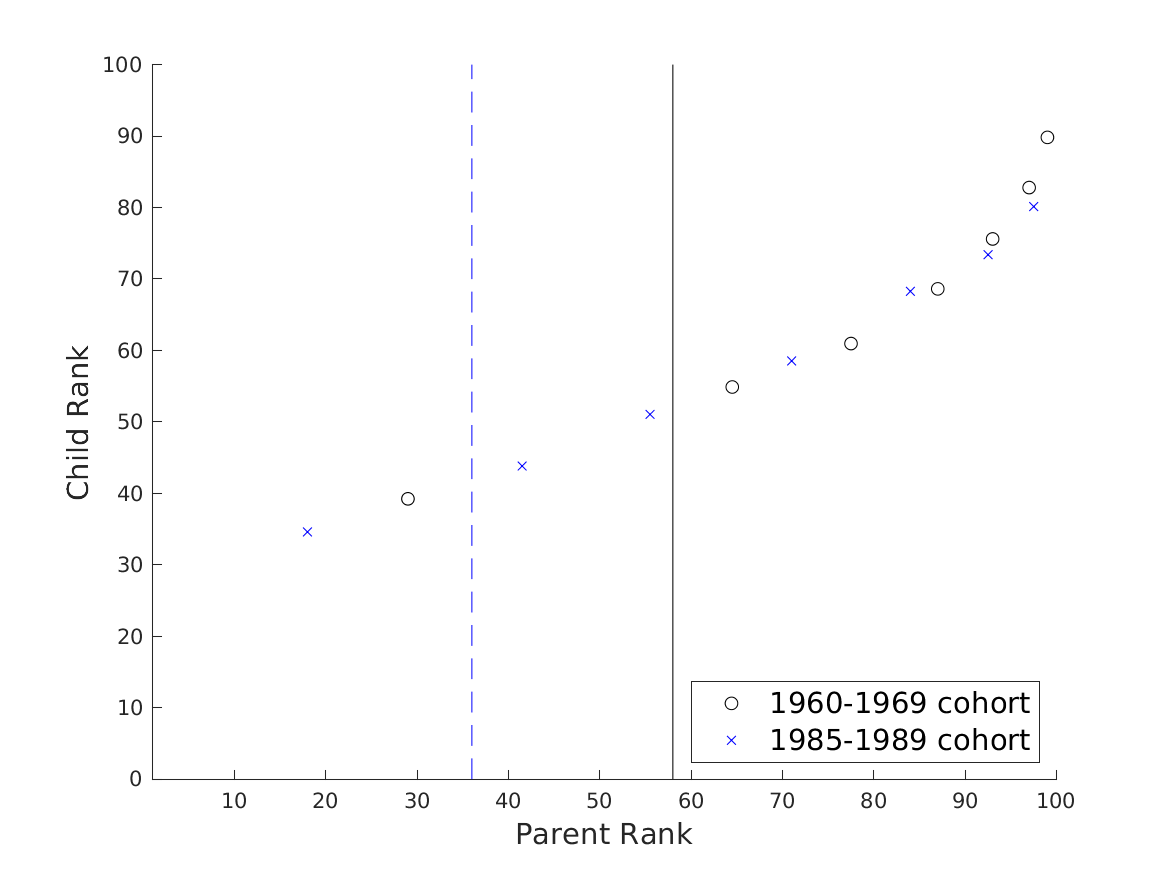
\includegraphics[scale=0.4]{\mobilitypath/moments_1960_1985.png}  & 
      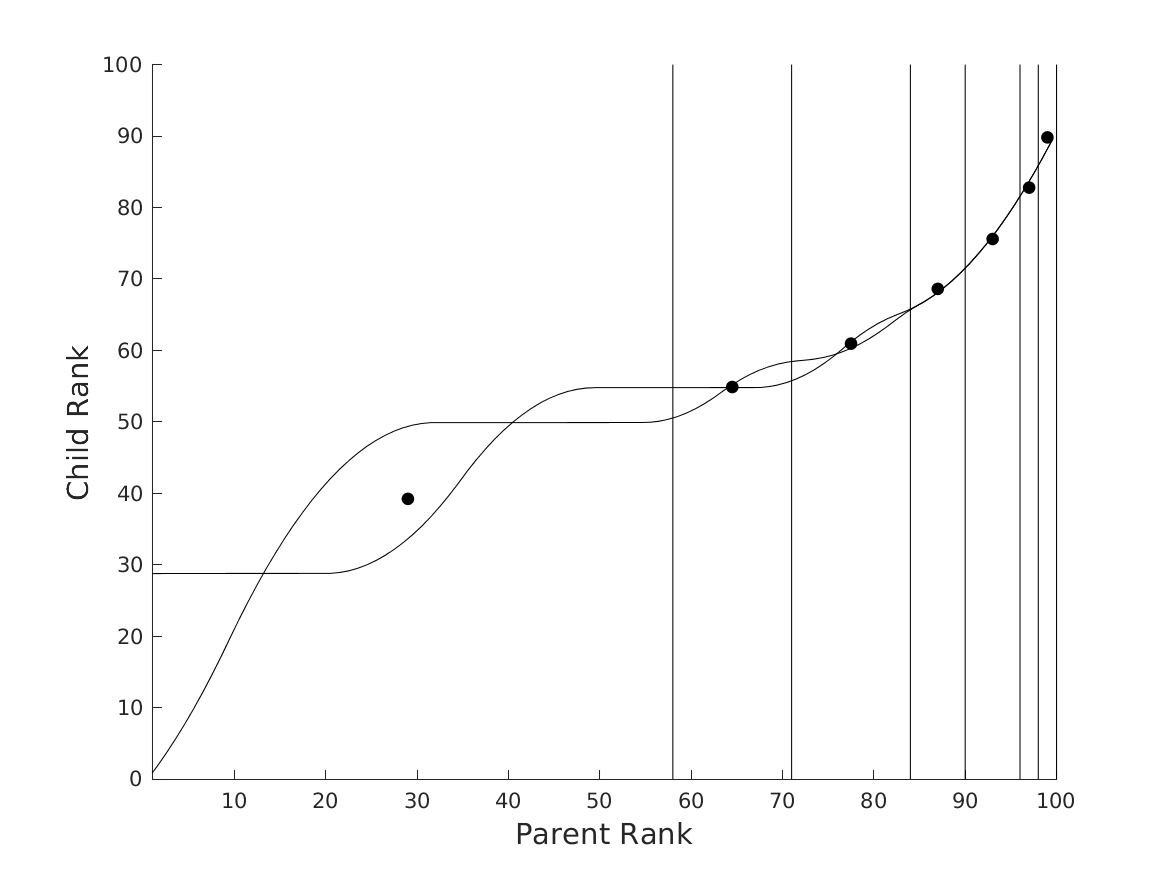
\includegraphics[scale=0.4]{\mobilitypath/fig_example_cef_1960.png} \\
\end{tabular}
\end{center}
\begin{center}
\begin{tabular}{c} 
    \panel{C. Partially Identified CEFs} \\ 
    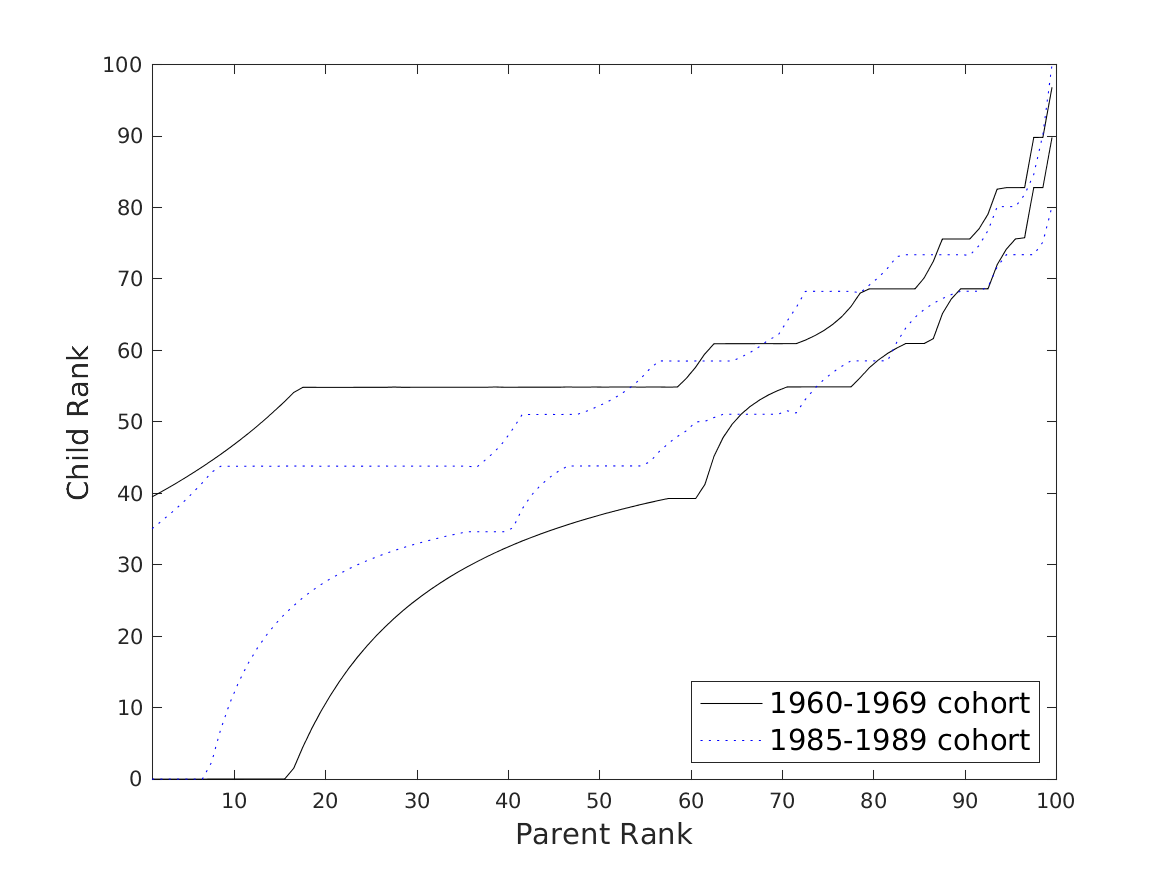
\includegraphics[scale=0.4]{\mobilitypath/fig_time_1960_25000.png}    
\end{tabular}
  \end{center}
  \newline
  \footnotesize{Panel A of the figure shows the average child
    education rank in each parent education rank bin for the 1960--69
    and 1985--89 birth cohorts. The vertical lines show the boundaries
    for the bottom parent bin, which corresponds to less than two
    years of education. The solid line corresponds to the 1960--69
    birth cohort and the dashed line to the 1985--89 birth
    cohort. Points are displayed at the midpoint of each parent
    rank bin. Panel B shows the 1960--69 moments again, along with two
    simulated conditional expectation functions which are equally good
    fits to the moments. Panel C shows bounds on father-son
  CEFs. Source: IHDS (2012).}
\end{figure}

%%%%%%%%%%%%%%%%%%%%%%%%%%%%%%%%%%%
%% ANNOTATED MU-0-50 EXPLANATION %%
%%%%%%%%%%%%%%%%%%%%%%%%%%%%%%%%%%%
\begin{landscape}
  \begin{figure}[H]
    \caption{Intuition: Calculating $\mu_0^{50}$ for 1960--69 Birth Cohort} 
    \label{fig:mu_annotation}

    \begin{center}
      \begin{tabular}{cc}
        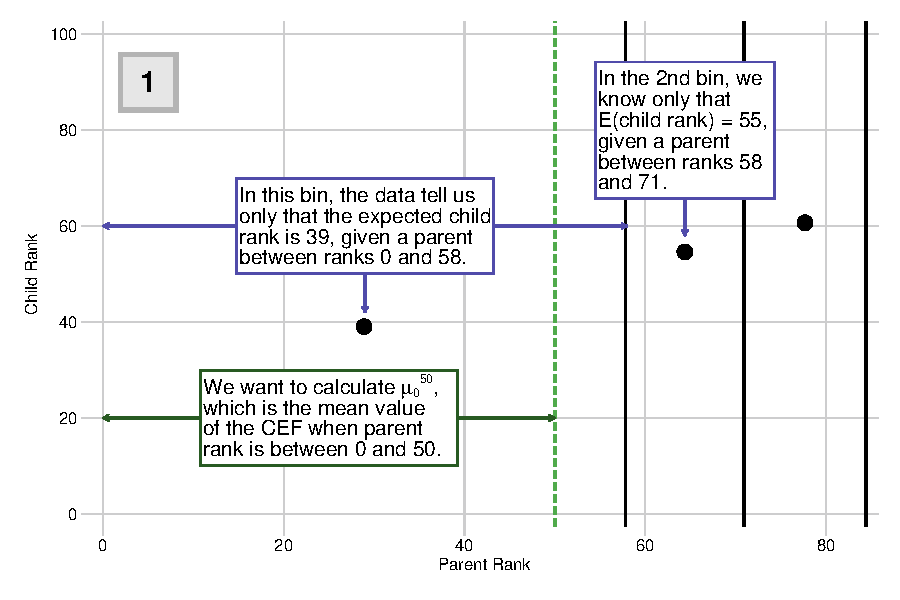
\includegraphics[scale=0.77]{\mobilitypath/example_ihds2} & 
        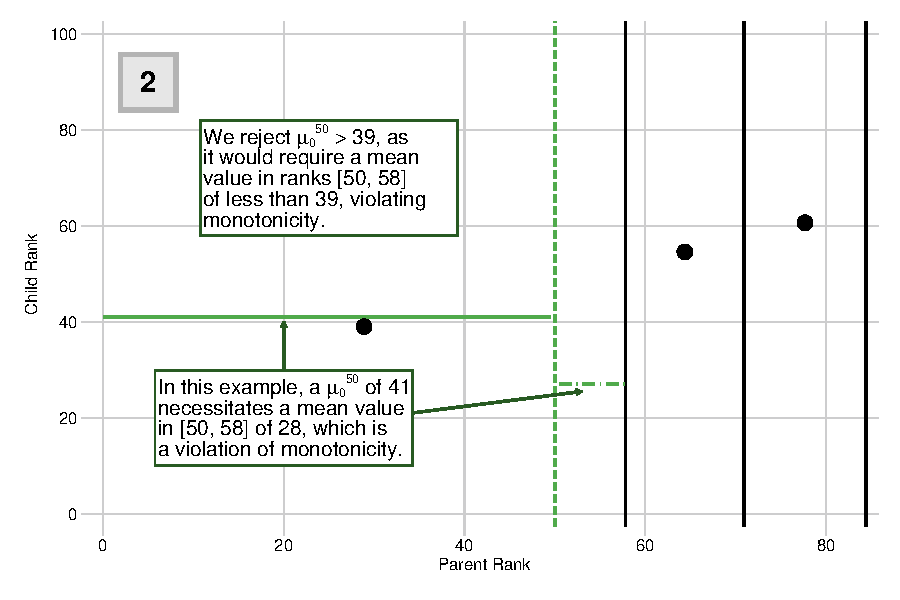
\includegraphics[scale=0.77]{\mobilitypath/example_ihds3} \\
        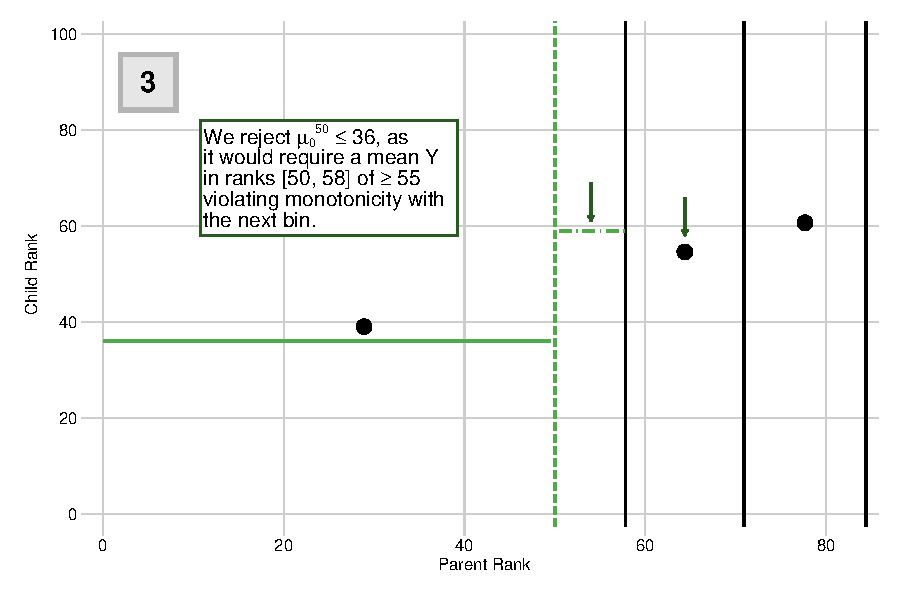
\includegraphics[scale=0.77]{\mobilitypath/example_ihds4} & 
        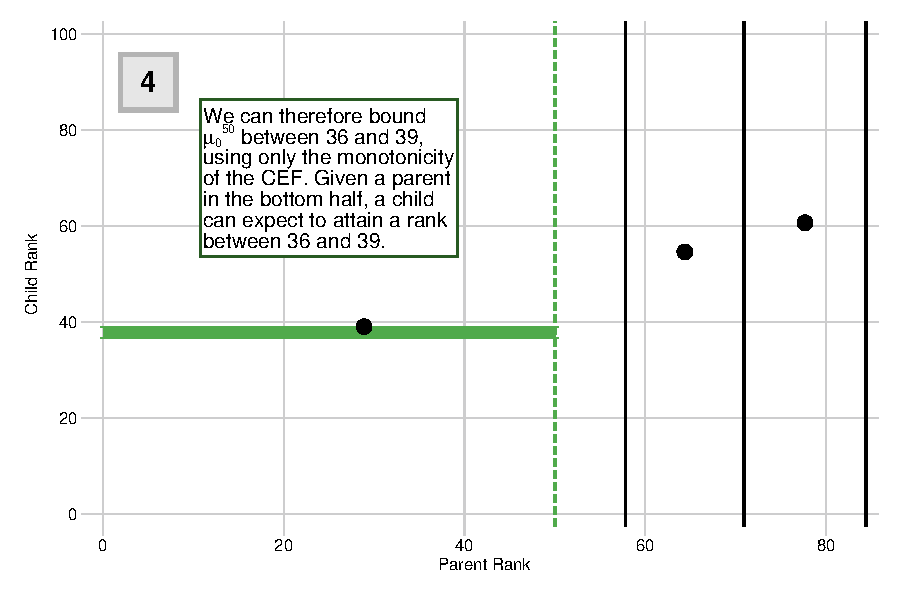
\includegraphics[scale=0.77]{\mobilitypath/example_ihds5} \\
      \end{tabular}          
    \end{center}
  \end{figure}
\end{landscape}

%%%%%%%%%%%%%%%%%%%%%%%%%%%%%%%%%%%%%
%% DESCRIPTIVE CHANGE IN EDUCATION %%
%%%%%%%%%%%%%%%%%%%%%%%%%%%%%%%%%%%%%
\begin{figure}[H]
  \caption{Changes in Educational Attainment by Birth Cohort} 
  \label{fig:descriptive_ed}
  \begin{center}
    \begin{tabular}{c} 
      \panel{A. Women} \\ 
      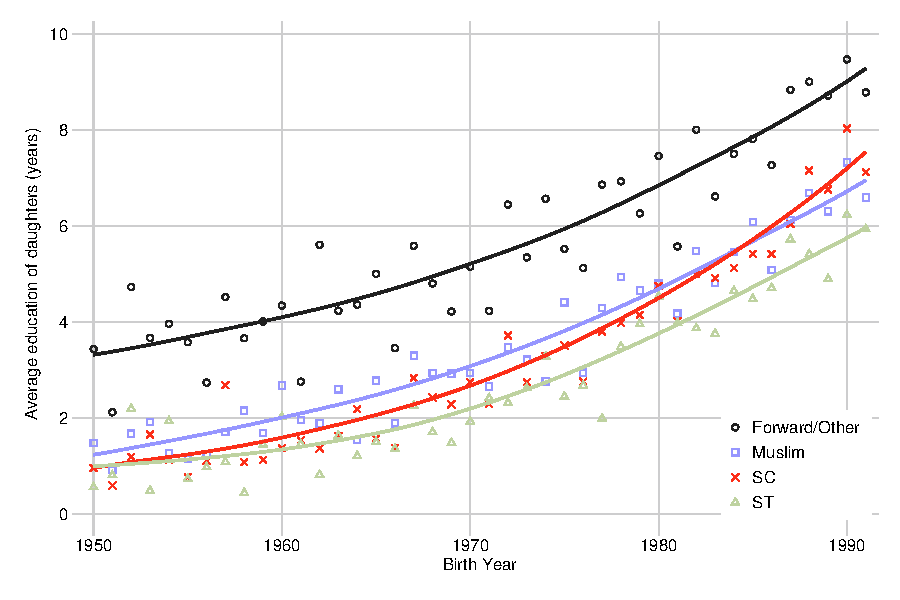
\includegraphics[scale=0.6]{\mobilitypath/daughter_ed_time} \\
      \panel{B. Men} \\ 
      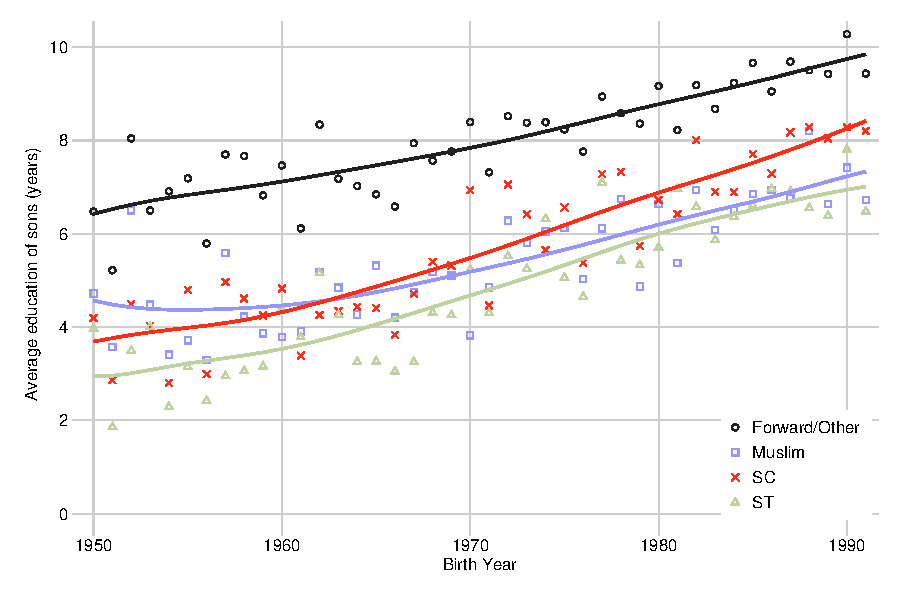
\includegraphics[scale=0.6]{\mobilitypath/son_ed_time} \\
    \end{tabular}
  \end{center}
  \footnotesize{The points show average levels of educational attainment for each birth cohort / social group. The lines are lowess curves fit to each group's time series. Source: IHDS (2012).}
\end{figure}

%%%%%%%%%%%%%%%%%%%%%%%%%%%%%%%%%%
%% BOUNDS ON p25, BETA, mu-0-50 %%
%%%%%%%%%%%%%%%%%%%%%%%%%%%%%%%%%%
\begin{landscape}
  \begin{figure}[H]
    \caption{Bounds on Father-Son Mobility Measures in India:\cnewline 1960--69 and 1985--89 Birth Cohorts}
    \label{fig:bounds_bpm}
    \begin{center}
      \begin{tabular}{ccc}
        \panel{A. Rank-Rank Gradient ($\beta$)}          &
        \panel{B. Absolute Upward Mobility  ($p_{25}$)}  &
        \panel{C. Bottom Half Mobility  ($\mu_0^{50}$)}  \\
        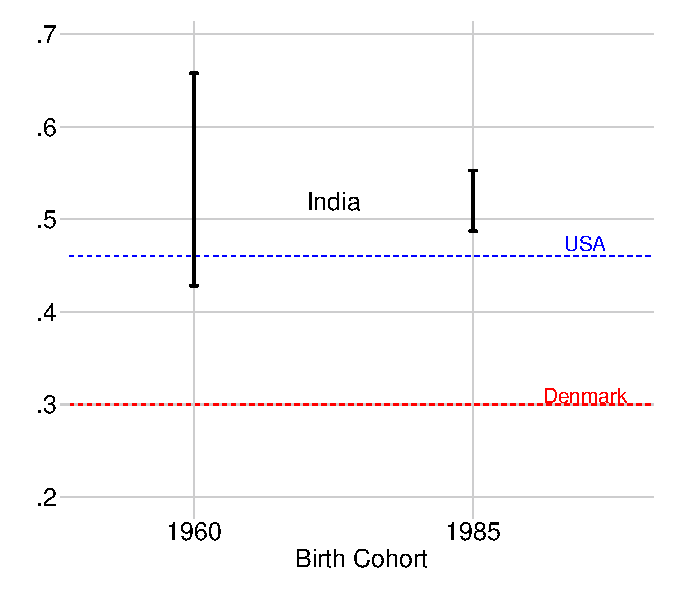
\includegraphics[scale=0.65]{\mobilitypath/gradient_60_85} &
        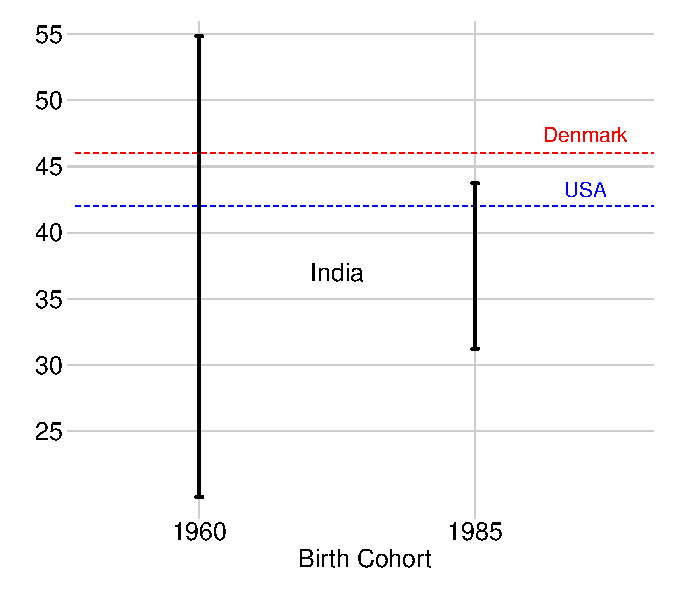
\includegraphics[scale=0.65]{\mobilitypath/p25_60_85} &
        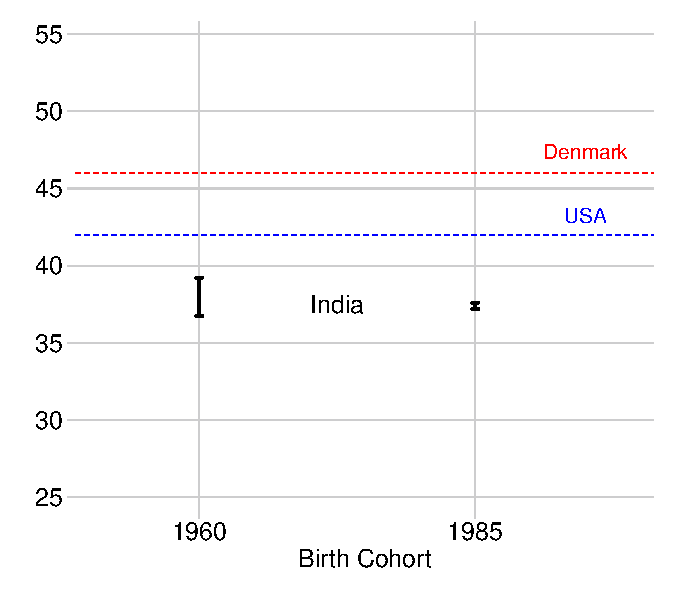
\includegraphics[scale=0.65]{\mobilitypath/mu50_60_85} \\
      \end{tabular}
      \hline
    \end{center}
    The figure shows bounds on three mobility statistics for the
    1960--69 and 1985--89 birth cohorts, estimated on father-son pairs
    in India. For reference, we display estimates of similar
    statistics from USA and Denmark. Data on rank-rank education
    gradients for USA and Denmark are from \citeasnoun{hertz2008}. For $p_{25}$ and
    $\mu_0^{50}$, the USA and Denmark references are \textit{income}
    mobility estimates from \citeasnoun{chetty2014c}. The Indian
    measures are all based on education data.  The rank-rank gradient
    is the slope coefficient from a regression of son education rank
    on father education rank. $p_{25}$ is absolute upward mobility,
    which is the expected rank of a son born to a father at the 25th
    percentile. $\mu_{0}^{50}$ is bottom half mobility, which is the
    expected rank of a son born to a father below the 50th
    percentile. Source: IHDS (2012).
  \end{figure}
\end{landscape} 

%%%%%%%%%%%
% TRENDS  %
%%%%%%%%%%%
\begin{figure}[H]
    \thispagestyle{empty}
  \caption{Bottom Half Mobility, 1950--1989 Birth Cohorts} 
  \label{fig:mu_gender}

  \begin{center}
    \begin{tabular}{cc}
      \panel{A. Father-Son Upward Mobility (Rank)}       &
      \panel{B. Father-Daughter Upward Mobility (Rank)}  \\
      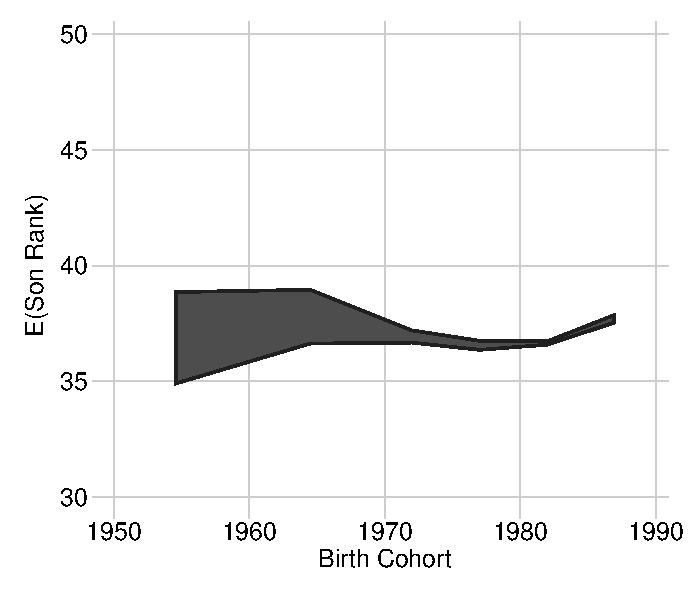
\includegraphics[scale=0.6]{\mobilitypath/ihds_mob_time_fs} &
      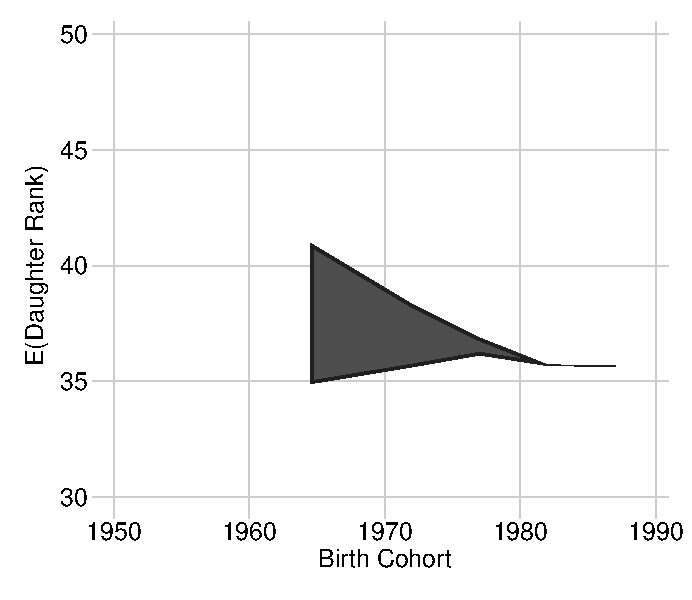
\includegraphics[scale=0.6]{\mobilitypath/ihds_mob_time_fd} \\
      \panel{C. Father-Son Mobility (Y = H.S.)} &
      \panel{D. Father-Daughter Mobility (Y = H.S.)}  \\
      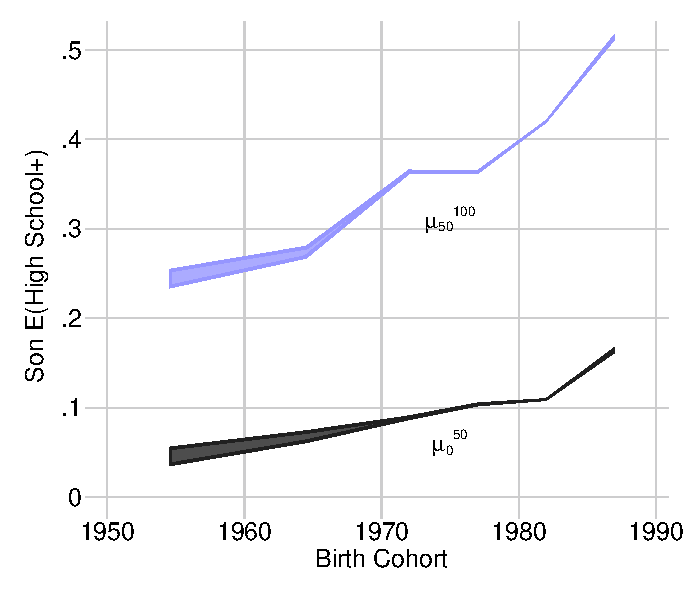
\includegraphics[scale=0.6]{\mobilitypath/ihds_mob_time_hs_m} &
      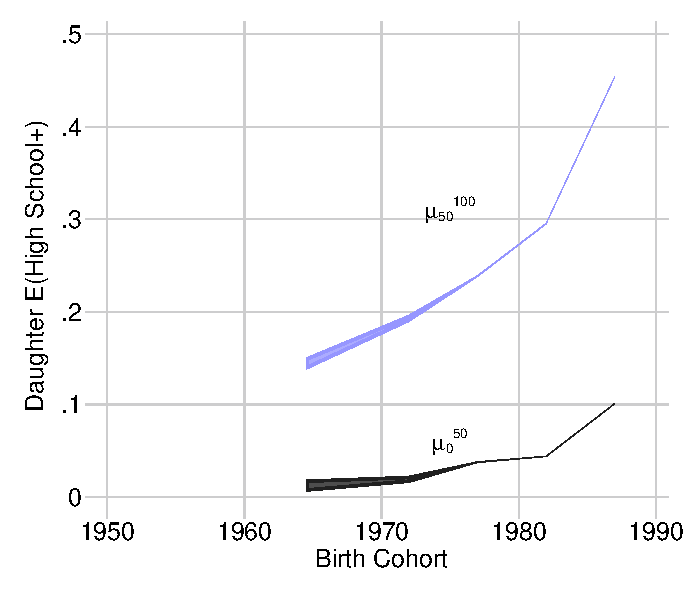
\includegraphics[scale=0.6]{\mobilitypath/ihds_mob_time_hs_f} \\
      \end{tabular}
  \end{center}

  \footnotesize{Figure \ref{fig:mu_gender} presents bounds on
    national intergenerational mobility, using cohorts born
    from 1950 through 1989. Panels A and B show bottom half mobility
    ($\mu_{0}^{50} = E(y|x \in [0, 50])$), where $x$ is parent rank and
    $y$ is child rank. This is the average rank attained by children
    born to parents who are in the bottom half of the education
    distribution, respectively for sons and daughters. Panels C and D
    show an analogous measure, $E(HS|x \in [0, 50])$ (gray) and
    $E(HS|x \in [50, 100])$ (blue). The first (gray) is the share of children
    completing high school, conditional on having parents in the
    bottom half of the education distribution. The second (blue) is the share
    of children completing high school, conditional on having parents in the
    top half of the parent distribution. Source: IHDS (2012).} 
\end{figure}

%%%%%%%%%%%%%%%%%%%%%%%%%%%%%%%%%%%%%%%%%%%%
%% TRENDS BY SOCIAL GROUP -- FATHER-CHILD %%
%%%%%%%%%%%%%%%%%%%%%%%%%%%%%%%%%%%%%%%%%%%%
\begin{figure}[H]
  \caption{Trends in Mobility by Subgroup, 1950--1989 Birth Cohorts} 
  \label{fig:group_mob}

  \begin{center}
    \begin{tabular}{cc}
      \panel{A. Father-Son Upward Mobility $\boldsymbol \mu_0^{50}$}  &
      \panel{B. Father-Son Downward Mobility $\boldsymbol \mu_{50}^{100}$}   \\
      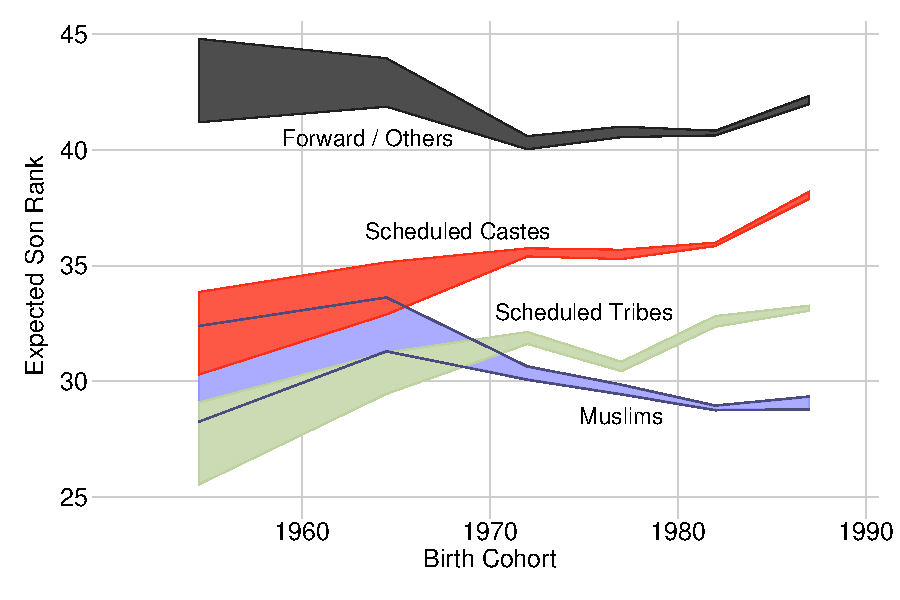
\includegraphics[scale=0.55]{\mobilitypath/ihds_mob_group_time_p25_m}
                                            & 
      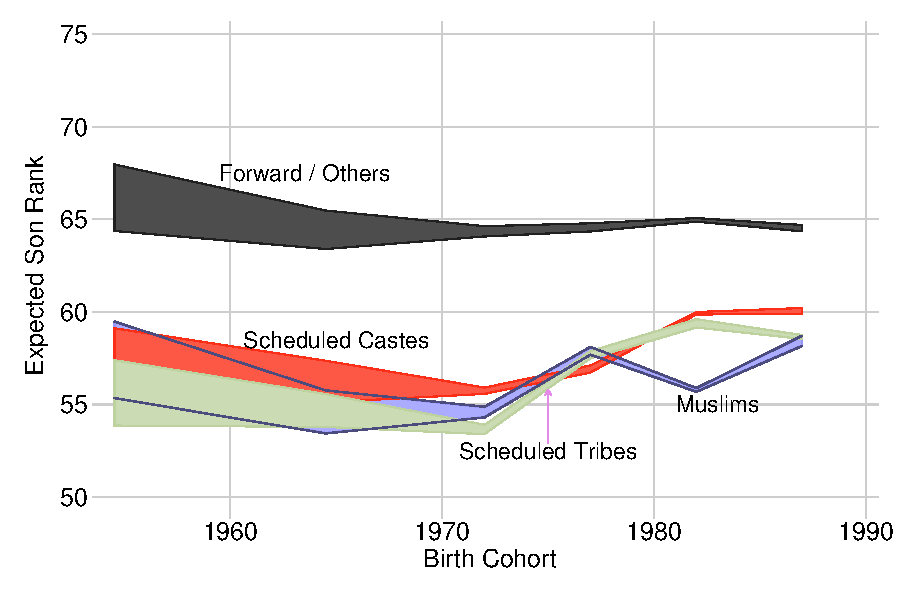
\includegraphics[scale=0.55]{\mobilitypath/ihds_mob_group_time_p75_m}  \\ 
      
      \panel{C. Father-Daughter Upward Mobility $\boldsymbol \mu_0^{50}$}  &
      \panel{D. Father-Daughter Downward Mobility $\boldsymbol \mu_{50}^{100}$}   \\
      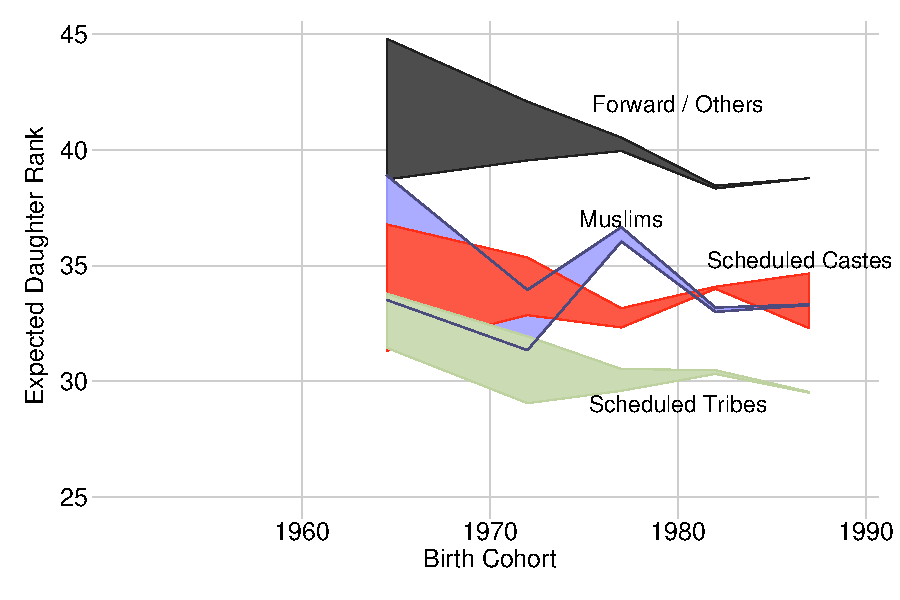
\includegraphics[scale=0.55]{\mobilitypath/ihds_mob_group_time_p25_f}
                                                 & 
      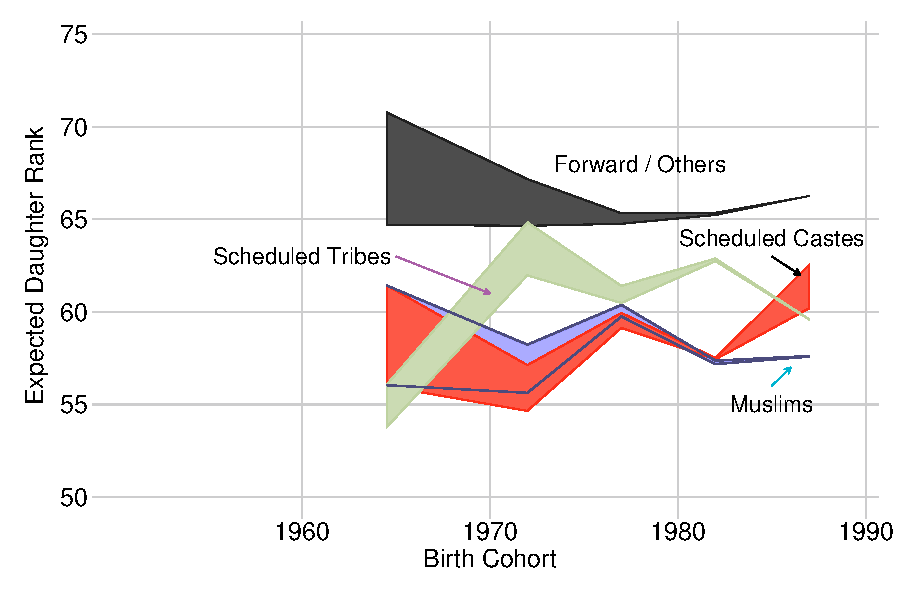
\includegraphics[scale=0.55]{\mobilitypath/ihds_mob_group_time_p75_f} \\
      \end{tabular}          
  \end{center}
  \newline
  \footnotesize{Figure~\ref{fig:group_mob} presents bounds on trends
    in intergenerational mobility, stratified by four prominent social
    groups in India: Scheduled Castes, Scheduled Tribes, Muslims, and
    Forward Castes/Others. The mobility measure in Panels A and C is
    bottom half mobility ($\mu_0^{50}$), or the average rank among
    children born to fathers in the bottom half of the father
    education distribution. The measure in Panels B and D is top half
    mobility ($\mu_{50}^{100}$), or the average rank among children
    born to fathers in top half of the father education
    distribution. Linked father-daughter education data are not
    available for the 1950--59 birth cohort.  Source: IHDS (2012).}
\end{figure}

%%%%%%%%%%%%%%%%%%%%%%%%%%%%%%%%%%
%% Affirmative action - cassan  %%
%%%%%%%%%%%%%%%%%%%%%%%%%%%%%%%%%%
\newpage 
\begin{figure}[H]
  \caption{Jati Redesignation and Intergenerational Mobility} 
  \label{fig:cassan}
  \begin{center}    
      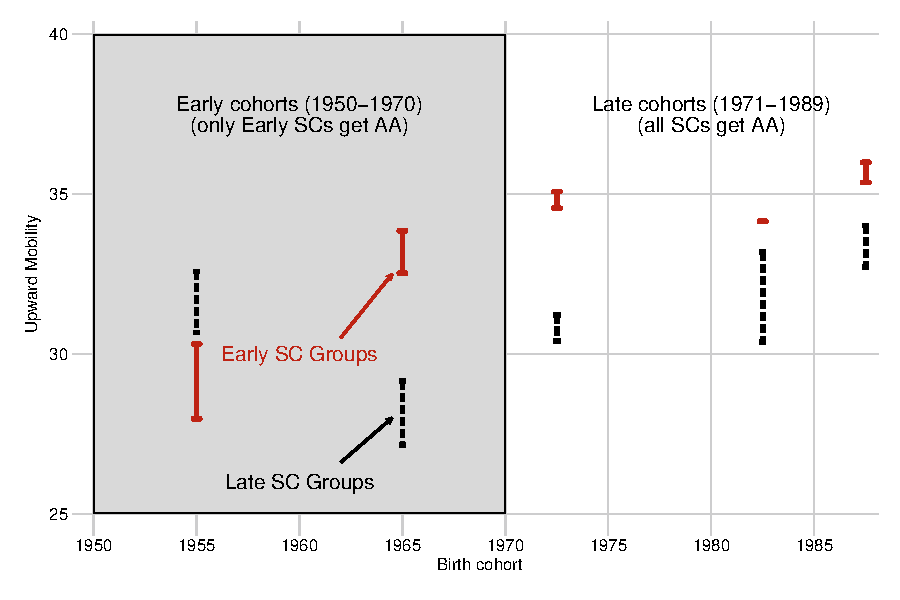
\includegraphics[scale=1.15]{\mobilitypath/jati_cohort_mob}
  \end{center}
  \newline
  \footnotesize{Figure~\ref{fig:cassan} shows bounds on bottom half
    mobility $\mu_0^{50}$ for two social groups in India. The dark red
    series shows upward mobility for groups that were designated as
    Scheduled Castes since before 1956. The black series shows
    upward mobility for groups that were not designated as Scheduled
    Castes until 1977; birth cohorts later than 1970 (outside the grey
    box) were six or younger when the policy change was implemented and thus would have had SC status at the primary school-starting age. Source: IHDS
    (2012).}
\end{figure}


  %%%%%%%%%%%%%%%%%%%%%%%
%% CHANGES OVER TIME %%
%%%%%%%%%%%%%%%%%%%%%%%
\begin{landscape}
\clearpage 
\pagestyle{fancy}
\markright{} 

\begin{table}
  \caption{Changes in Upward Mobility Over Time}
  \label{tab:mob_changes}
  \begin{center}
    \panel{A. Father-son pairs}
  \end{center}
\begin{center}
  \begin{tabular}{cccccc} 
\hline
\hline
& All groups & Forward/Others & Muslims & SCs & STs \\
\hline 
1960--1969 & [36.6, 39.0] &
[41.8, 44.0] &
[31.3, 33.6] &
[32.9, 35.2] & 
[29.4, 31.3] \\ 
& \{35.7, 39.8\} &
\{40.6, 45.3\} &
\{29.4, 35.6\} &
\{31.3, 36.8\} & 
\{27.0, 33.7\} \\ 
& & & & & \\ 
1980--1989 & [37.1, 37.2] &
[41.3, 41.3] &
[28.9, 29.0] &
[36.9, 37.0] & 
[33.1, 33.1] \\ 
& \{36.4, 37.8\} &
\{40.3, 42.3\} &
\{27.7, 30.2\} &
\{35.5, 38.5\} & 
\{31.2, 35.1\} \\ 
& & & & & \\ 
Change over time & [-1.9, 0.6] &
[-2.7, -0.5] &
[-4.7, -2.3] &
[1.8, 4.1] & 
[1.8, 3.7] \\ 
& \{-3.0, 1.7\} &
\{-4.3, 1.1\} &
\{-7.0, -0.0\} &
\{-0.4, 6.3\} & 
\{-1.3, 6.8\} \\ 
Fraction overlapping bounds & 0.818 & 
0.310 & 0.054 & 0.090 & 0.119 \\ 
\hline
\hline 
\end{tabular}
 
\end{center}
  \begin{center}
    \panel{B. Father-daughter pairs}
  \end{center}
\begin{center}
  \begin{tabular}{cccccc} 
\hline
\hline
& All groups & Forward/Others & Muslims & SCs & STs \\
\hline 
1960--1969 & [34.9, 41.0] &
[38.7, 44.8] &
[33.5, 38.9] &
[31.3, 36.8] & 
[31.4, 33.8] \\ 
& \{34.1, 41.8\} &
\{37.6, 45.9\} &
\{31.8, 40.6\} &
\{29.8, 38.3\} & 
\{29.0, 36.2\} \\ 
& & & & & \\ 
1980--1989 & [35.4, 35.5] &
[38.0, 38.2] &
[32.0, 33.5] &
[32.9, 34.2] & 
[30.4, 30.5] \\ 
& \{34.6, 36.3\} &
\{36.8, 39.3\} &
\{30.9, 34.6\} &
\{31.7, 35.4\} & 
\{28.3, 32.6\} \\ 
& & & & & \\ 
Change over time & [-5.6, 0.6] &
[-6.9, -0.5] &
[-6.9, -0.0] &
[-3.9, 2.9] & 
[-3.4, -0.9] \\ 
& \{-6.7, 1.7\} &
\{-8.4, 1.0\} &
\{-8.8, 1.9\} &
\{-5.8, 4.8\} & 
\{-6.6, 2.2\} \\ 
Fraction overlapping bounds & 0.781 & 
0.244 & 0.434 & 0.985 & 0.346 \\ 
\hline
\hline 
\end{tabular}
 
\end{center}
\\ 
\footnotesize{Table~\ref{tab:mob_changes} shows estimates of full
    sample and subgroup bottom half mobility ($\mu_0^{50}$) for the
    1960--69 and 1980--89 birth cohorts for father-son (Panel A) and
    father-daughter (Panel B) pairs. We show both bounds (in square
    brackets) and 90\% confidence sets (in curly braces) on those
    bounds. The table also reports the bounds and 90\% confidence sets
    on the change in bottom half mobility between these two time
    periods. We obtain confidence sets by generating 1,000 bootstrap
    draws, estimating bounds on each bootstrap draw, and following the
    framework in \citeasnoun{cherno2007} to form 90\% confidence
    sets from bootstrapped bounds. Because these are
    confidence sets rather than confidence
    intervals, instead of $p$-values we show the fraction of bootstraps
    in which the 1960--69 and 1980--89 bounds are overlapping. Source:
    IHDS (2012).}
\end{table}
\end{landscape} 
%%%%%%%%%%%%%%%%%%%%%%%
%% GROUP DIFFERENCES %%
%%%%%%%%%%%%%%%%%%%%%%%
\clearpage
\pagestyle{fancy}

\begin{table}[H]
  \caption{Group Differences in Upward Mobility}
  \label{tab:group_diffs}
  \hline
\hline
\begin{tabular}{cccc} 
& F/O minus SC & F/O minus Muslim & SC minus Muslim \\ 
\hline 
Father/son ($\mu_0^{50}$) & [4.6, 5.0] &
                            [11.6, 12.1] &
                            [6.9, 7.3] \\
& \{2.8, 6.8\} &
  \{10.0, 13.8\} &
  \{4.5, 9.6\} \\
Fraction overlapping bounds & 0.000  & 0.000 & 0.000 \\ 
\hline

Father/daughter ($\mu_0^{50}$) & [4.2, 4.5] &
                                 [5.1, 5.5] &
                                 [0.8, 1.1] \\
& \{1.9, 6.8\} &
  \{2.9, 7.7\} &
  \{-2.0, 3.9\} \\
Fraction overlapping bounds & 0.001  & 0.000 & 0.511 \\ 
\hline

Father/son ($\mu_{50}^{100}$) & [4.8, 5.3] &
                                [9.0, 9.4] &
                                [3.9, 4.3] \\
& \{3.3, 6.8\} &
  \{5.8, 12.6\} &
  \{0.8, 7.5\} \\
Fraction overlapping bounds & 0.000  & 0.000 & 0.005 \\ 
\hline

Father/daughter ($\mu_{50}^{100}$) & [7.7, 8.0] &
                                [7.8, 8.2] &
                                [0.0, 0.4]  \\
 & \{4.0, 11.7\} &
   \{5.3, 10.8\} &
   \{-3.9, 4.3\} \\
Fraction overlapping bounds & 0.000  & 0.000 & 0.318 \\ 
\end{tabular}
\hline
\hline 


  \newline
  \newline
  \footnotesize{Table~\ref{tab:group_diffs} shows estimates of
    cross-group differences in bottom half mobility ($\mu_0^{50}$) and
    top half mobility ($\mu_{50}^{100}$) in the 1980--89 birth
    cohorts. F/O stands for Forwards/Others and SC for Scheduled Castes. We show both bounds (in square brackets) and 90\% confidence sets (in curly braces) on those bounds. We obtain confidence sets by generating 1,000 bootstrap draws, estimating
    bounds on each bootstrap draw, and following the framework in
    \citeasnoun{cherno2007} to form 90\% confidence sets from
    bootstrapped bounds. Because these are confidence sets rather than
    confidence intervals, instead of $p$-values we show the fraction
    of the bounds for the two social groups that are overlapping. For
    example, the value of 0.509 in the final column indicates that
    50.9\% of the bootstraps generate overlapping bounds for the two
    groups. Source: IHDS (2012).}
\end{table}

%%%%%%%%%%%%%%%%%%
%% CASSAN TABLE %%
%%%%%%%%%%%%%%%%%%
\begin{table}[H]
  \caption{Effect of Scheduled Caste Designation on Upward Mobility}
  \label{tab:mech_cassan}
  \begin{center}
    \begin{tabular}{c}
    \panel{A. Father-son pairs} \\
    \setlength{\linewidth}{.1cm} \begin{center}
\newcommand{\contents}{\begin{tabular}{l*{3}{c}}
\hline\hline
                    &         (1)   &         (2)   &         (3)   \\
\hline
Post * Late SC      &       8.432***&       6.764***&               \\
                    &     (1.794)   &     (1.555)   &               \\
1970-79 * Late SC   &               &               &       6.739** \\
                    &               &               &     (2.025)   \\
1980-89 * Late SC   &               &               &       9.649***\\
                    &               &               &     (2.580)   \\
N                   &        4502   &        3746   &        4502   \\
r2                  &        0.32   &        0.34   &        0.32   \\
\hline
\multicolumn{4}{p{\linewidth}}{$^{*}p<0.10, ^{**}p<0.05, ^{***}p<0.01$} \\
\multicolumn{4}{p{\linewidth}}{\footnotesize \tablenote}
\end{tabular} }
\setbox0=\hbox{\contents}
\setlength{\linewidth}{\wd0-2\tabcolsep-.25em} \contents \end{center}
 \\
    \panel{B. Father-daughter pairs} \\
    \setlength{\linewidth}{.1cm} \begin{center}
\newcommand{\contents}{\begin{tabular}{l*{3}{c}}
\hline\hline
                    &         (1)   &         (2)   &         (3)   \\
\hline
Post * Late SC      &      -3.183   &      -1.604   &               \\
                    &     (1.645)   &     (1.666)   &               \\
1970-79 * Late SC   &               &               &      -2.658   \\
                    &               &               &     (1.727)   \\
1980-89 * Late SC   &               &               &      -1.685   \\
                    &               &               &     (2.342)   \\
N                   &        3429   &        3040   &        3177   \\
r2                  &        0.34   &        0.33   &        0.33   \\
\hline
\multicolumn{4}{p{\linewidth}}{$^{*}p<0.10, ^{**}p<0.05, ^{***}p<0.01$} \\
\multicolumn{4}{p{\linewidth}}{\footnotesize \tablenote}
\end{tabular} }
\setbox0=\hbox{\contents}
\setlength{\linewidth}{\wd0-2\tabcolsep-.25em} \contents \end{center}
 \\
    \end{tabular}
  \end{center}
  
  \footnotesize{Table~\ref{tab:mech_cassan} shows estimates from Equation~\ref{eq:cassan}, which describes the impact of Scheduled Caste designation on upward mobility. The dependent variable is the child education rank. The sample consists of SC children of fathers in approximately the bottom 60\% of the education distribution. \textit{Late SC} is an indicator for jati groups that were added to Scheduled Caste lists in the caste redesignation of 1977. \textit{Post} is an indicator for cohorts born after 1970. The sample in Panel A is all men, while Panel B is all women. In the Column 1 estimation, the are 696 ``late SC'' men, of whom 438 were born after 1970. For women, these numbers are 516 and 391 respectively. All estimations control for region $\times$ cohort, jati $\times$ region, jati $\times$ cohort, and birth year, and are clustered at the jati and the region levels. Source: IHDS (2012).}
\end{table}



  \section{Appendix A: Additional Tables and Figures}
  \setcounter{table}{0}
  \renewcommand{\thetable}{A\arabic{table}}
  \setcounter{figure}{0}
  \renewcommand{\thefigure}{A\arabic{figure}}

  %%%%%%%%%%%%%%%%%%%%%%%%%%%%%%
% CORESIDENCE RATES FOR M/F  %
%%%%%%%%%%%%%%%%%%%%%%%%%%%%%%
\begin{figure}[H]
  \caption{Coresidence Rates by Age and Gender} 
  \label{fig:cores_rates}
  \begin{center}
    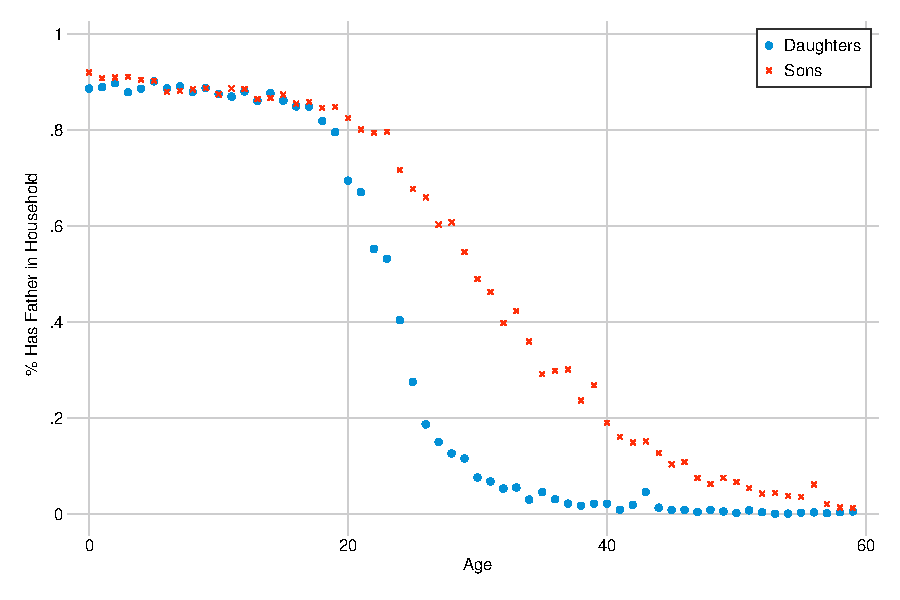
\includegraphics[scale=0.5]{\mobilitypath/cores_age}
  \end{center}
  \newline
  \footnotesize{Figure~\ref{fig:cores_rates} shows the share of
    individuals who live in the same household as their father as a
    function of gender and age. Source: IHDS (2012).}  
\end{figure}

%%%%%%%%%%%%%%%%%%%%%%%%%%%%%%%%%%%%%%
% CORESIDENCE BIAS IN MOB ESTIMATES  %
%%%%%%%%%%%%%%%%%%%%%%%%%%%%%%%%%%%%%%
\begin{figure}[h]
  \caption{Bias in Mobility Estimates When Sample is Limited to Coresident Pairs} 
  \label{fig:cores_bias}

  \begin{center}
    \begin{tabular}{cc}
      A. Father-Son Pairs &        B. Father-Daughter Pairs  \\
      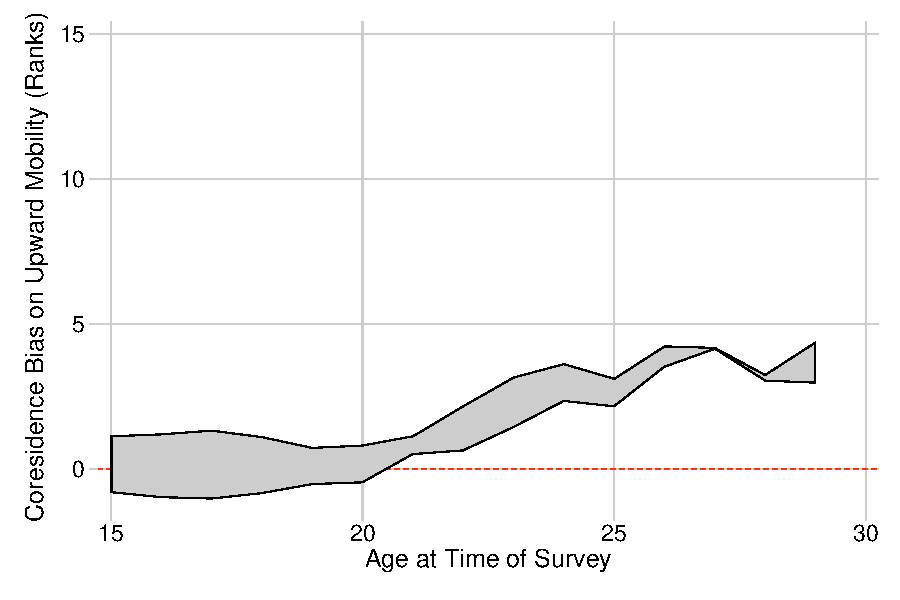
\includegraphics[scale=0.45]{\mobilitypath/cores_bias_upward_m} & 
      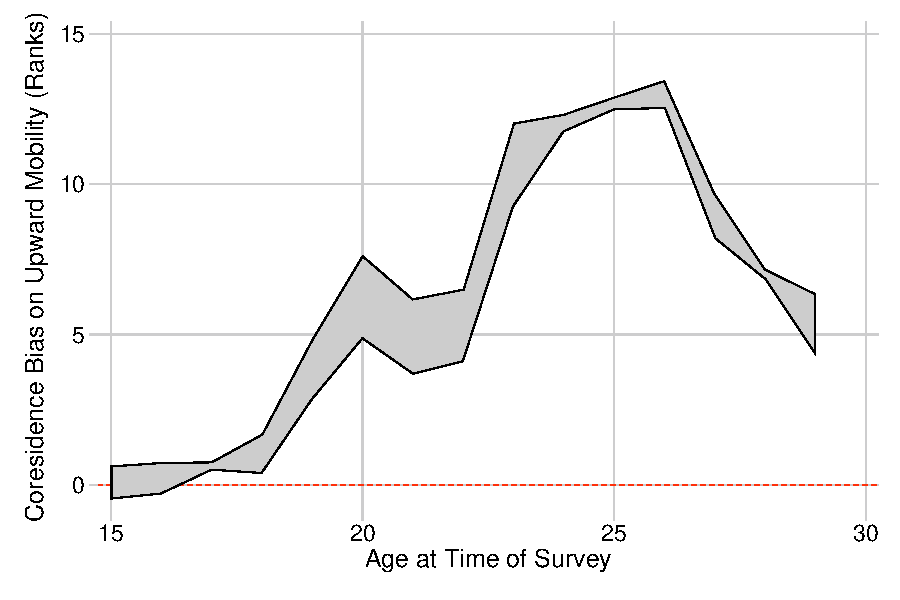
\includegraphics[scale=0.45]{\mobilitypath/cores_bias_upward_f} \\
      \end{tabular}          
  \end{center}
  \newline
  \footnotesize{Figure~\ref{fig:cores_bias} shows the bias in a
    measure of upward mobility when children who do not live with
    their parents are excluded from the sample. The bias is shown as a function of
    child age. The mobility measure is bottom half mobility
    ($\mu_0^{50}$), which is the expected child rank conditional on
    being born to a parent in the bottom half of the education
    distribution. Bias is calculated as the coresident-only measure
    minus the full sample measure. Source: IHDS (2012).}
\end{figure}

%%%%%%%%%%%%%%%%%%%%%%%%%%%%%%
%% RANK-RANK SCATTER GRAPHS %%
%%%%%%%%%%%%%%%%%%%%%%%%%%%%%%
\begin{landscape}
  \begin{figure}[h]
    \vspace{-2cm}
  \caption{Joint Parent-Child Education Moments Over Time} 
  \label{fig:rank_scatters}

  \begin{center}
    \begin{tabular}{cc}
      \panel{A. Father-Son Pairs} &       \panel{B. Father-Daughter Pairs} \\ 
      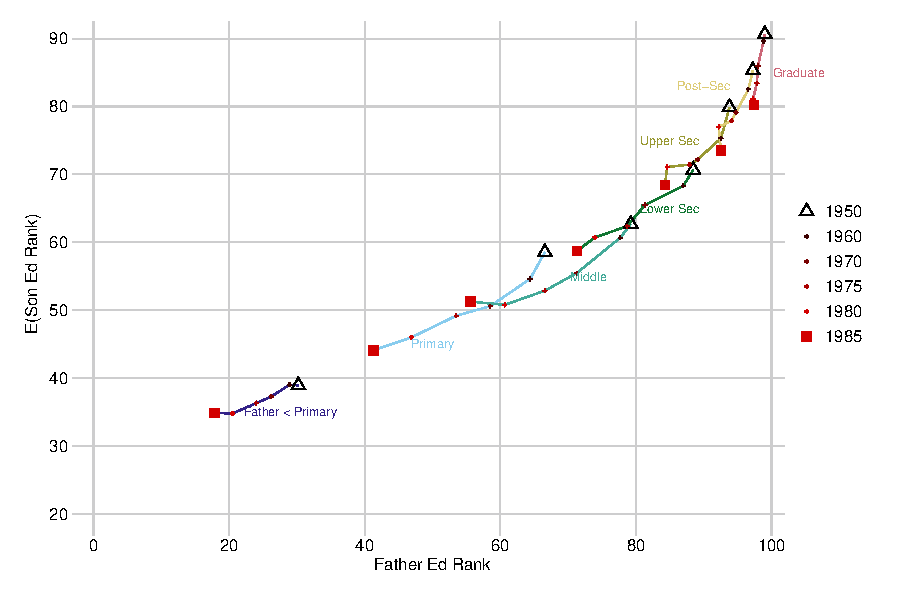
\includegraphics[scale=0.7]{\mobilitypath/scatter_father_son} & 
      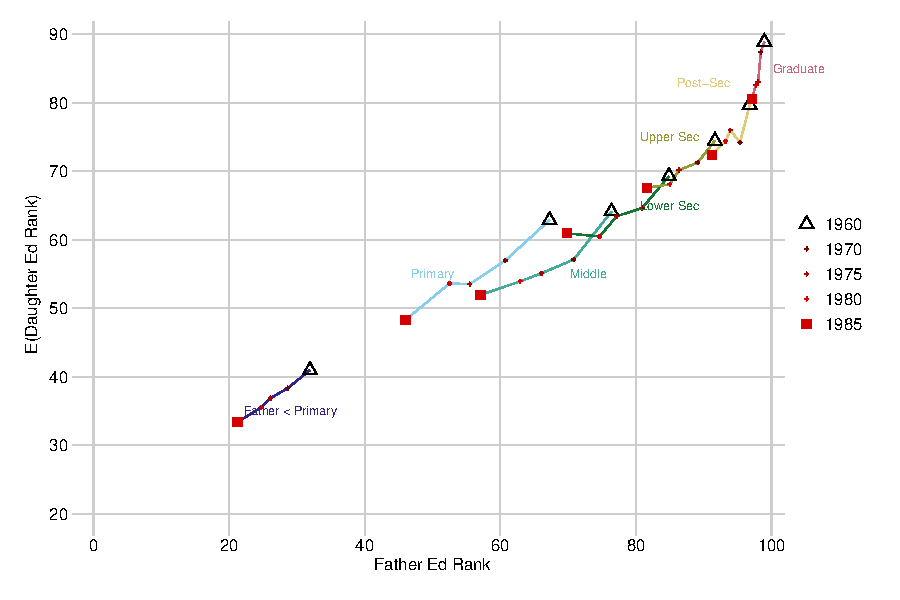
\includegraphics[scale=0.7]{\mobilitypath/scatter_father_daughter} \\
      \panel{C. Mother-Son Pairs} &       \panel{D. Mother-Daughter Pairs} \\ 
      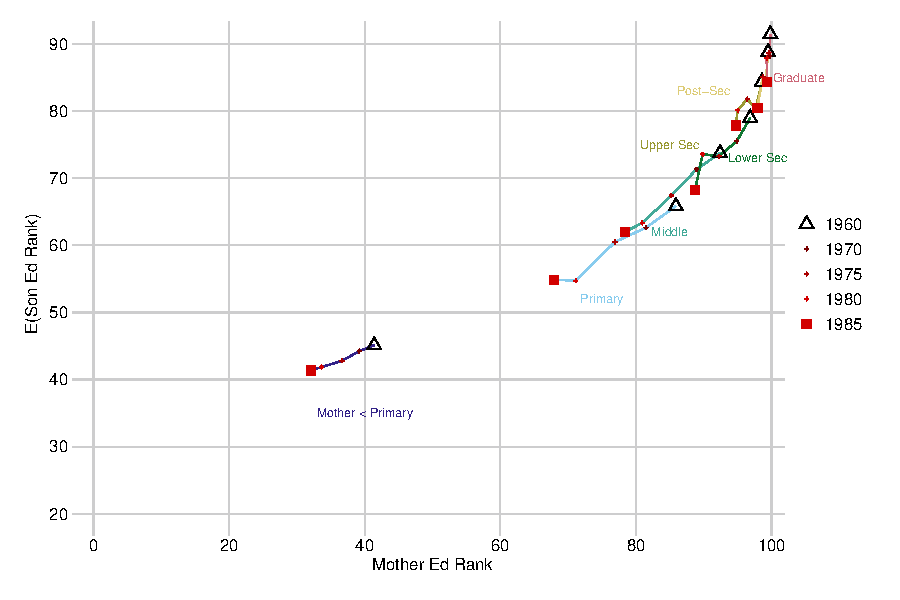
\includegraphics[scale=0.7]{\mobilitypath/scatter_mother_son} & 
      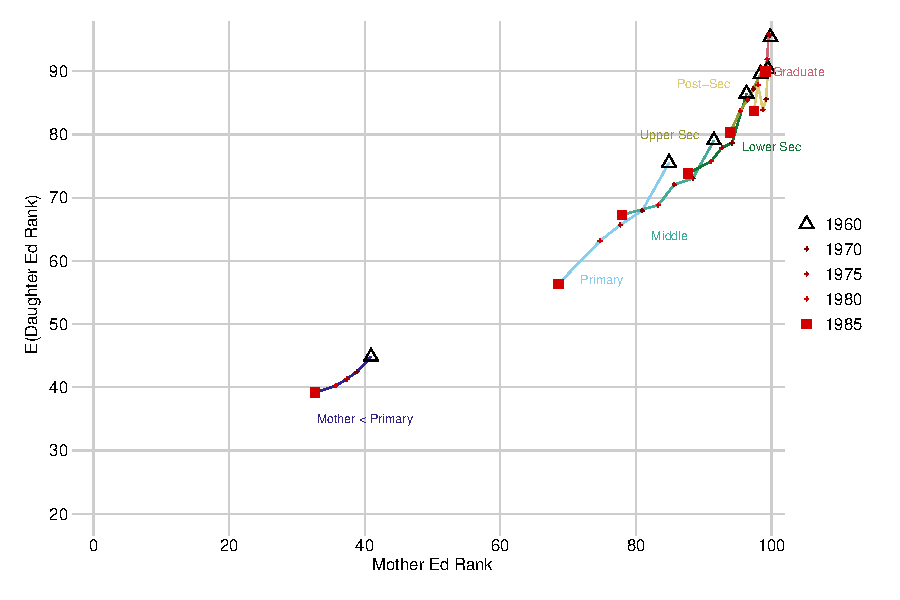
\includegraphics[scale=0.7]{\mobilitypath/scatter_mother_daughter} \\
    \end{tabular}
  \end{center}
  \newline
  \footnotesize{The figure shows the conditional expectation function of child education rank, given parent education rank for six cohorts. Each set of connected points corresponds to a time series for a different \textit{level} of education; the time series (which moves from the triangle to the square) shows changes in a child's expected rank (Y axis) given a parent at some fixed level of education, along with the change in the father's education rank (X axis) in the cohort of fathers. Points move to the southwest because low-education fathers have lower ranks as education rises (moving left), and thus have children with lower education ranks (moving down). Ranks are calculated as the midpoint rank of a given education bin. Source: IHDS (2012).}
\end{figure}
\end{landscape}
\resetgeometry
%%%%%%%%%%%%%%%%%%%%%%%%%%%%%%%%%%%%%%%%%%%
%% SURVIVOR BIAS: IHDS 2005 vs IHDS 2011 %%
%%%%%%%%%%%%%%%%%%%%%%%%%%%%%%%%%%%%%%%%%%%
\newpage 
\begin{figure}[H]
  \caption{Robustness of Upward Mobility to Survivorship Bias} 
  \label{fig:mob_survivor}

  \begin{center}
    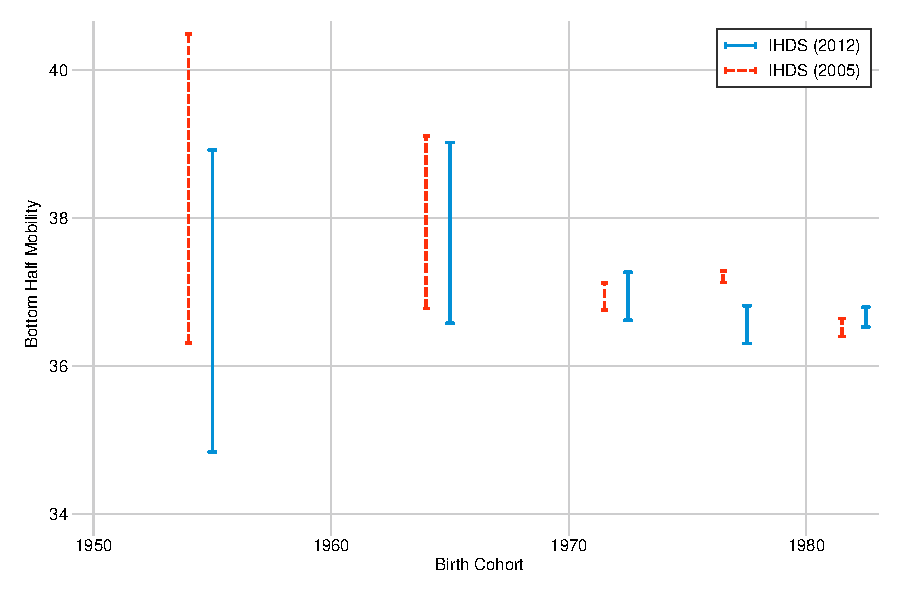
\includegraphics[scale=0.5]{\mobilitypath/mob_survivor} \\
  \end{center}
  \footnotesize{Figure \ref{fig:mob_survivor} shows a test of
    survivorship bias in estimates of bottom half mobility. The figure
    shows estimates of bottom half mobility calculated for the 1950s to 1980--85
    birth cohorts, measured separately in the 2005 and 2012 rounds of the IHDS. If there
    was substantial survivorship bias in the mobility measures, we
    would expect the estimates to differ across the two surveys
    because of the deaths of some of the respondents.}
\end{figure}

%%%%%%%%%%%%%%%%%%%%%
%% MOTHERS MU-0-50 %%
%%%%%%%%%%%%%%%%%%%%%
\begin{figure}[h]
  \caption{Bottom Half Mobility ($\mu_0^{50}$) for Mother-Son and
    Mother-Daughter Pairs } 
  \label{fig:mob_moms_mu50}

  \begin{center}
    \begin{tabular}{cc}
      A. Mother-Son Pairs &       B. Mother-Daughter Pairs \\ 
      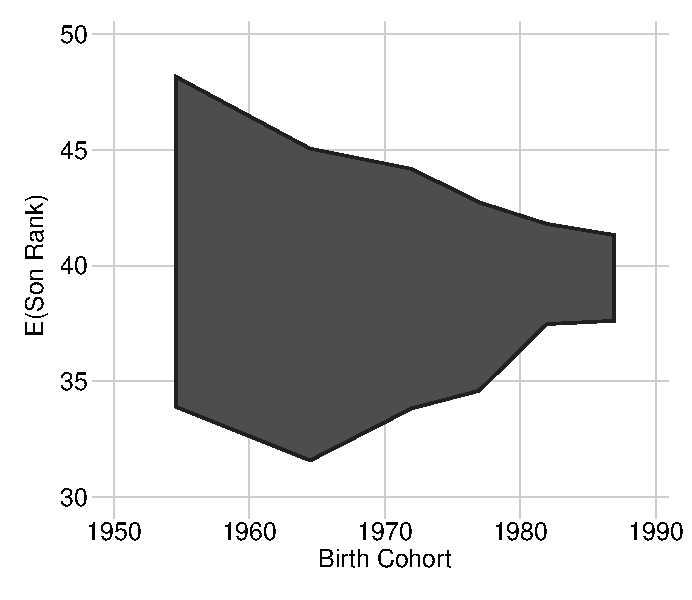
\includegraphics[scale=0.5]{\mobilitypath/ihds_mob_time_ms} & 
      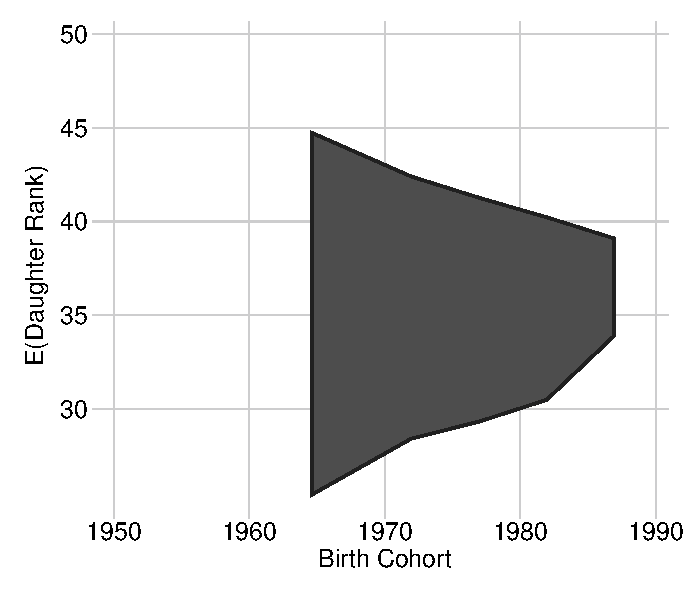
\includegraphics[scale=0.5]{\mobilitypath/ihds_mob_time_md} \\
      \end{tabular}          
  \end{center}
  \newline
  \footnotesize{Figure \ref{fig:mob_moms_mu50} shows bounds on
    aggregate trends in intergenerational mobility, using cohorts born
    from 1950--59 through 1985--89, focusing on mother-son and
    mother-daughter links. The measure used is bottom half mobility
    ($\mu_{0}^{50}$), which is the average rank attained by children
    born to parents who are in the bottom half of the education
    distribution. The bounds are very wide because of the large share
    of mothers who report bottom-coded education levels. Source: IHDS (2012).}
\end{figure}

%%%%%%%%%%%%%%%%%%%%%%%%%%%%%%%%%%%%%%%%%%%%%%
%% TRENDS BY SOCIAL GROUP -- LEVEL OUTCOMES %%
%%%%%%%%%%%%%%%%%%%%%%%%%%%%%%%%%%%%%%%%%%%%%%
\clearpage
\newpage 
\begin{figure}[H]
  \caption{Trends in Mobility by Subgroup, 1950--1989 Birth Cohorts
    \cnewline Education Level Outcomes} 
  \label{fig:group_mob_levels}

  \begin{center}
    \begin{tabular}{cc}
      
      \panel{A. Father-Son, Primary School $\boldsymbol \mu_0^{50}$} &
      \panel{B. Father-Daughter, Primary School $\boldsymbol \mu_0^{50}$}    \\ 
      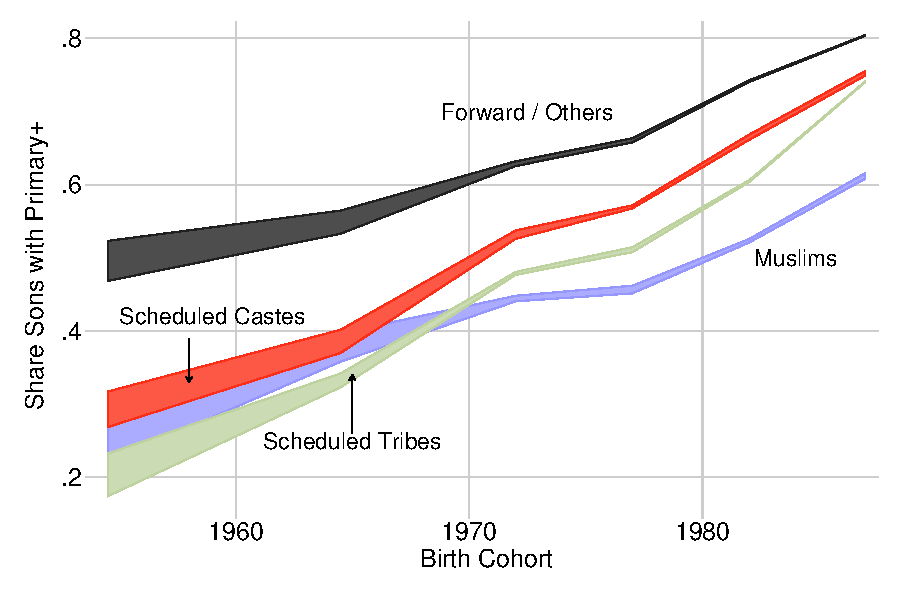
\includegraphics[scale=0.55]{\mobilitypath/ihds_mob_group_time_p25_prim_m} &
      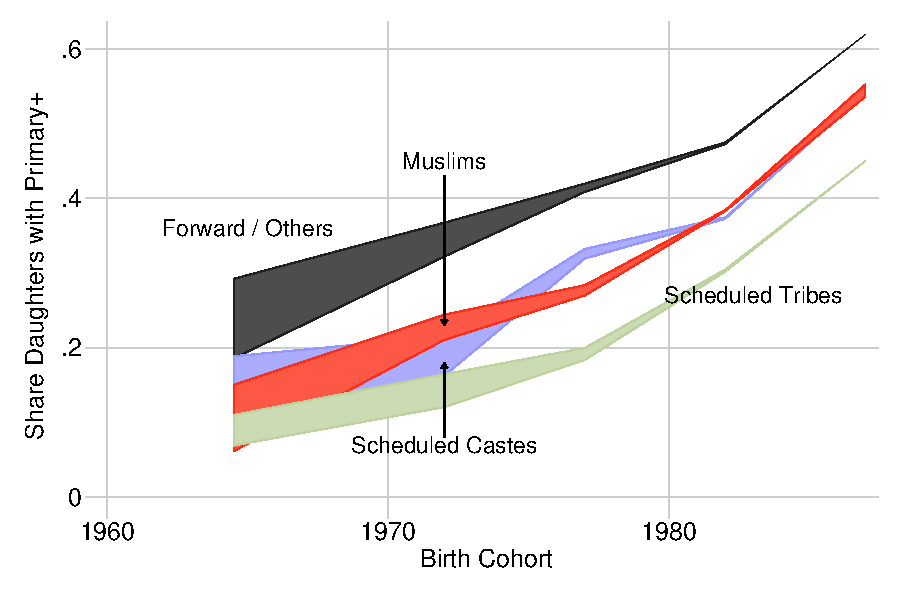
\includegraphics[scale=0.55]{\mobilitypath/ihds_mob_group_time_p25_prim_f}
      \\
      
      \panel{C. Father-Son, High School $\boldsymbol \mu_0^{50}$} &
      \panel{D. Father-Daughter, High School $\boldsymbol \mu_0^{50}$}    \\ 
      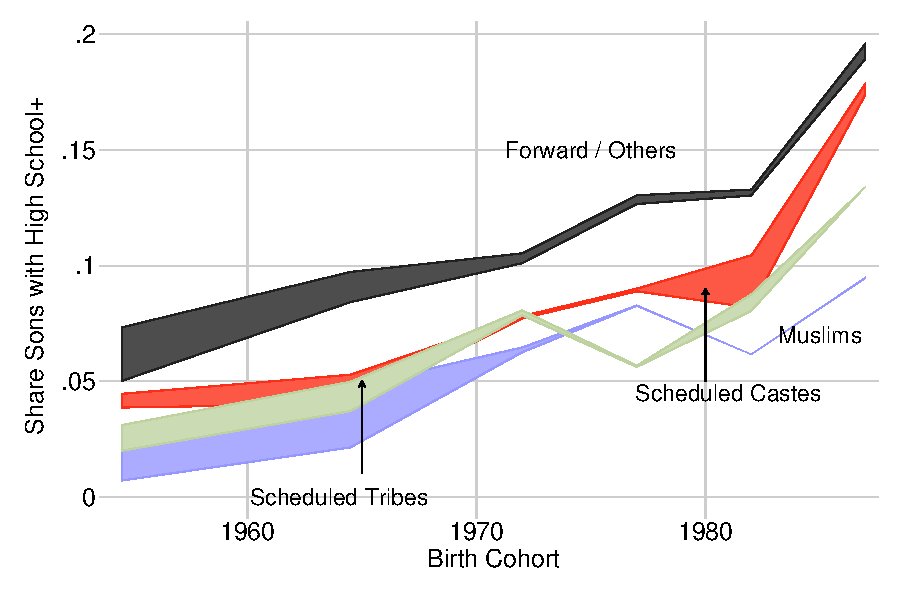
\includegraphics[scale=0.55]{\mobilitypath/ihds_mob_group_time_p25_hs_m} &
      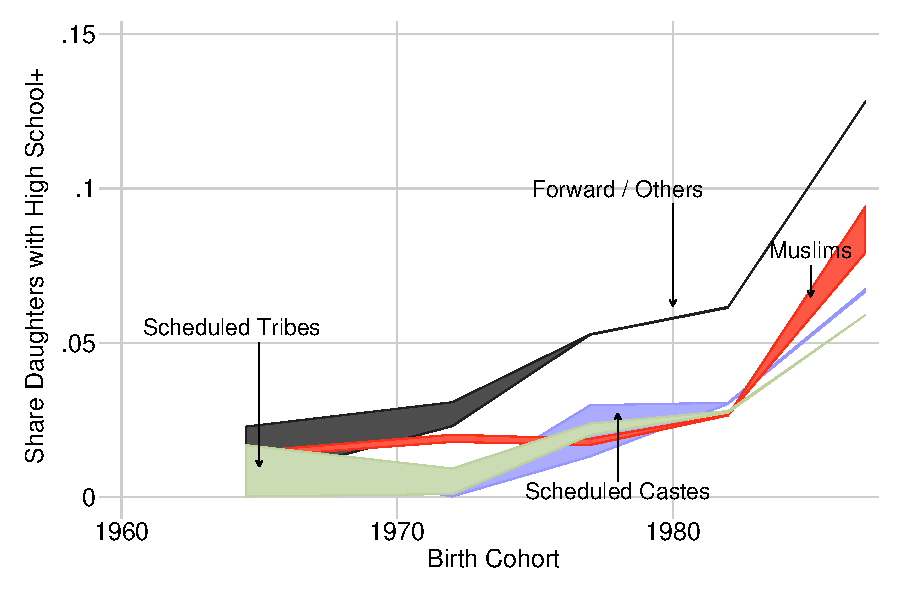
\includegraphics[scale=0.55]{\mobilitypath/ihds_mob_group_time_p25_hs_f}
      \end{tabular}          
  \end{center}
  \newline
  \footnotesize{Figure \ref{fig:group_mob_levels} presents bounds on 
    intergenerational mobility, stratified by four prominent social
    groups in India: Scheduled Castes, Scheduled Tribes, Muslims, and
    Forward Castes/Others. The figure is analogous to
    Figure~\ref{fig:group_mob}, but shows the expected probability that a child
    attains a given education level (primary
    in Panels A and B, and secondary in Panels C
    and D), conditional on having a 
    father in the bottom half of the father education
    distribution. Linked father-daughter education data are not
    available for the 1950--59 birth cohort.
    Source: IHDS (2012).}
\end{figure}

%%%%%%%%%%%%%%%%%%%%%%%%%%%%%%%%%%%%%%%%%%%%%%%%%%%%%%%%%%%%%%%%
%% Cassan affirmative action spec with a range of post values %%
%%%%%%%%%%%%%%%%%%%%%%%%%%%%%%%%%%%%%%%%%%%%%%%%%%%%%%%%%%%%%%%%
\newpage 
\begin{figure}[H]
  \caption{Effect of Scheduled Caste Designation on Upward Mobility \cnewline
  Robustness to Alternate Post Years} 
  \label{fig:aa_by_post}

  \begin{center}
    \begin{tabular}{c}
      \panel{A. Father-son pairs} \\
      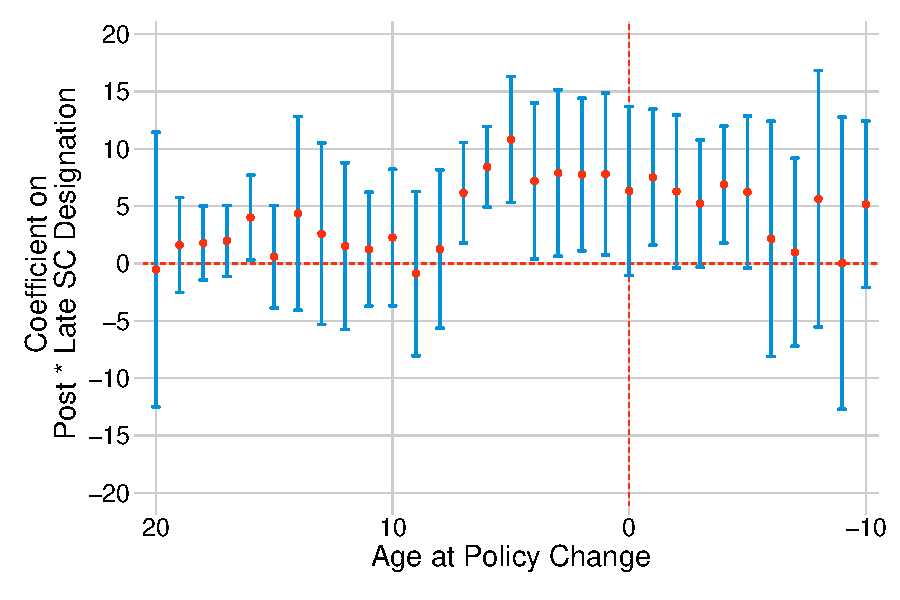
\includegraphics[scale=0.55]{\mobilitypath/aa_time_series_boy} \\
      \panel{B. Father-daughter pairs} \\
      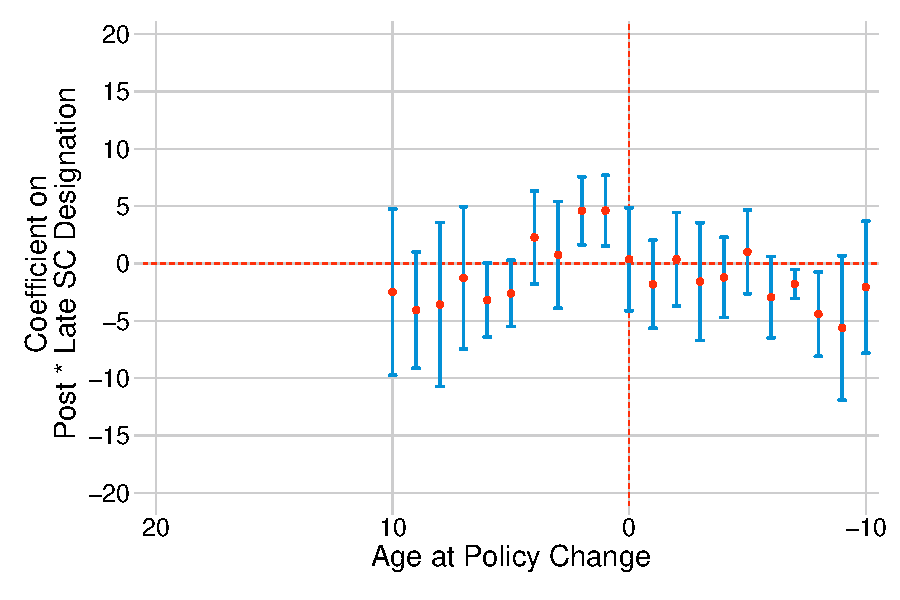
\includegraphics[scale=0.55]{\mobilitypath/aa_time_series_girl}
      \end{tabular}          
  \end{center}
  \newline
  \footnotesize{The figure shows point estimates from Equation~\ref{eq:cassan}, with a range of definitions of ``post'', the first year at which post-policy-change cohorts are modeled as exposed to the new policy regime. The X axis shows the child's age at the time of the policy change in 1977; negative ages describe children born after 1977. All outcomes are measured in 2012. The Y axis shows a regression coefficient which describes the relative gains in rank points to ``Late'' Scheduled Caste children born after their castes were added to the Scheduled Caste list (see Section~\ref{sec:cassan}). Source: IHDS (2012).}
\end{figure}

%%%%%%%%%%%%%%%%%%%%%%%%%%%%%%%%%%%%%%%%%%%%%%%%%%%
%% Rejected mechanisms for mobility differences  %%
%%%%%%%%%%%%%%%%%%%%%%%%%%%%%%%%%%%%%%%%%%%%%%%%%%%
\begin{landscape} 
\begin{figure}
\caption{Other Candidate Mechanisms}
  \label{fig:mechanisms}
  \begin{center}
    \begin{tabular}{cc}
      \panel{A. Within-State and Within-District Social Group Mobility Gaps}  &
      \panel{B. Mincerian Returns for Different Social Groups}  \\
      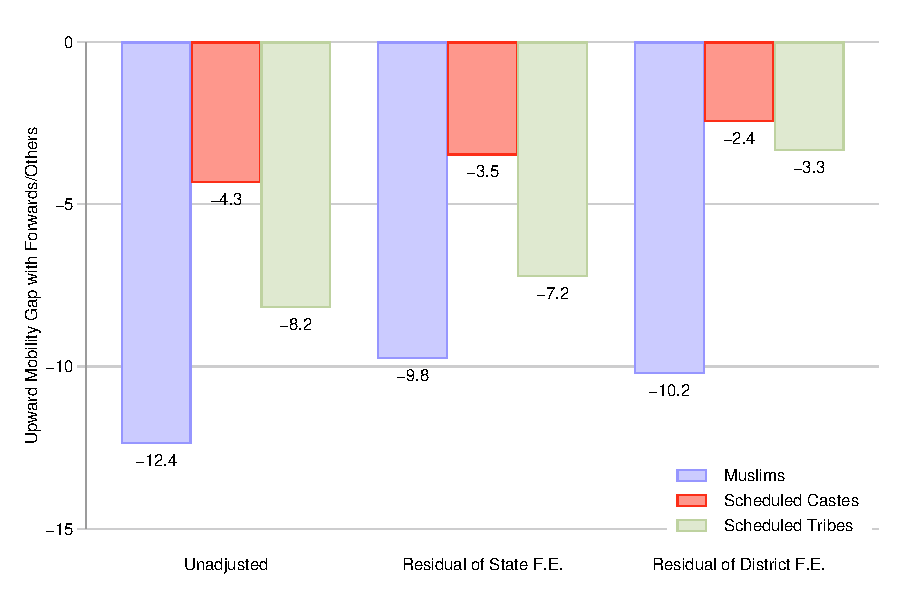
\includegraphics[scale=0.65]{\mobilitypath/mob_gaps_sd_resids} &
      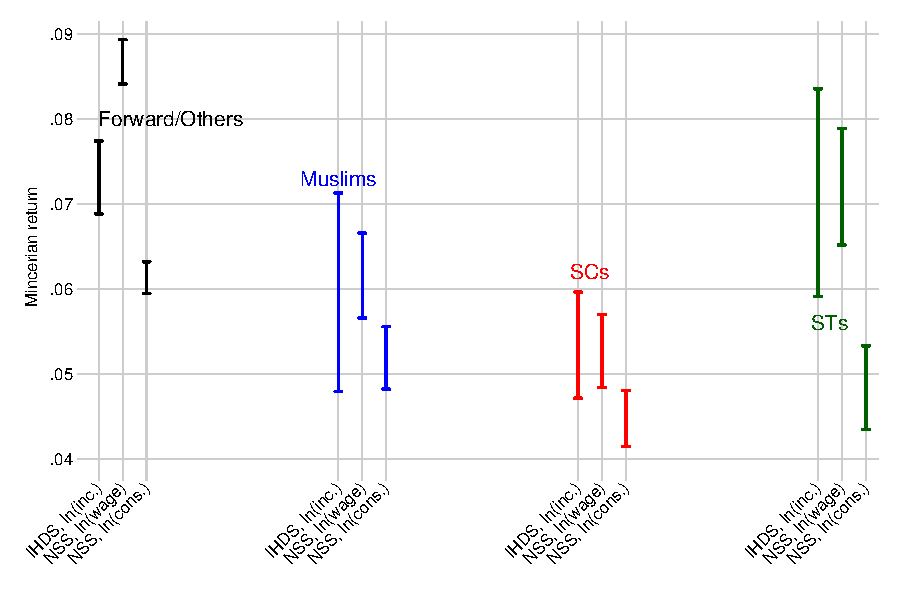
\includegraphics[scale=0.65]{\mobilitypath/mincerian_returns_pooled_4} \\
      \panel{C. Business Ownership by Demographic Group} &
      \panel{D. Mobility by Business Ownership} \\
      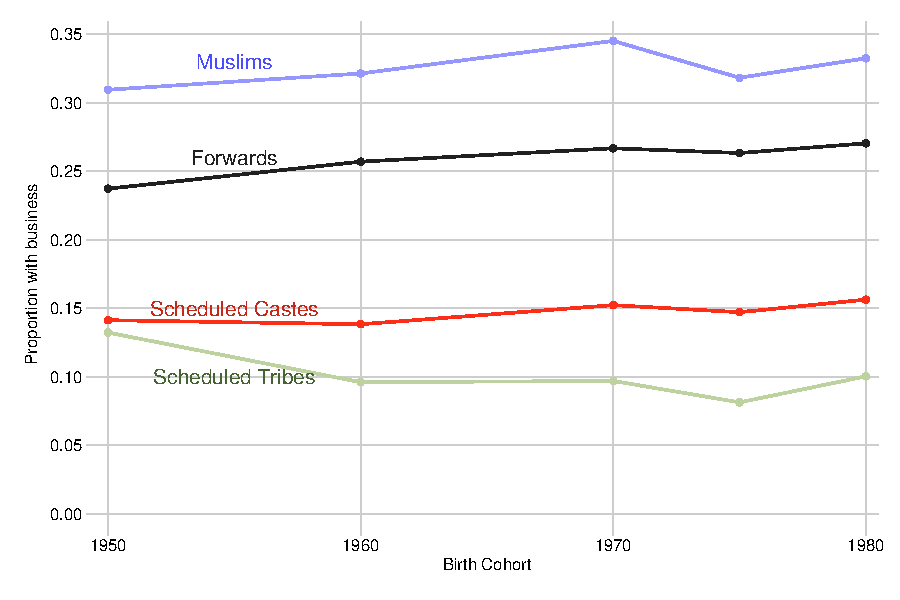
\includegraphics[scale=0.65]{\mobilitypath/has_business_ts} & 
      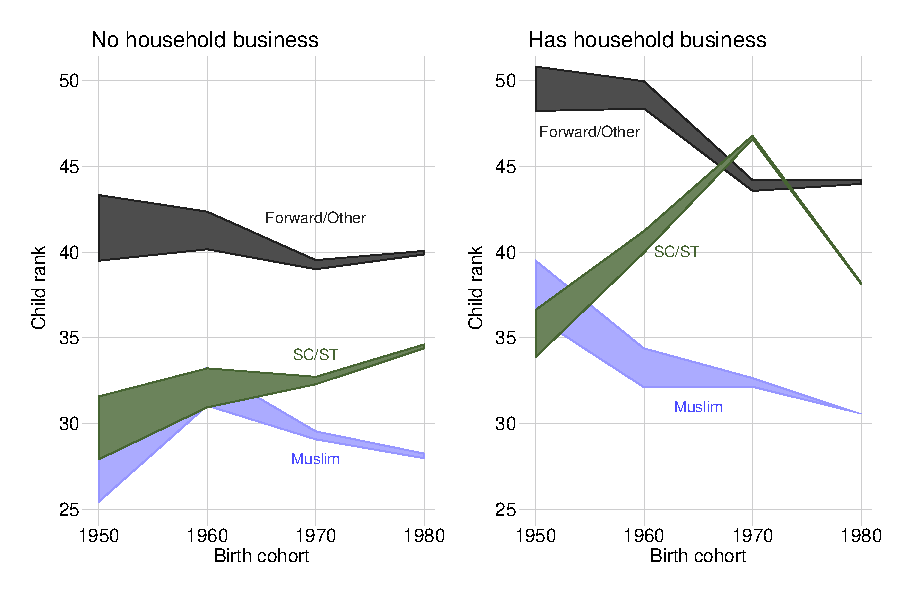
\includegraphics[scale=0.65]{\mobilitypath/mob_by_own_business} \\
  \end{tabular}
\end{center}
  \newline
  \tiny{Panel A presents the bottom-half mobility disadvantage relative to Forwards/Others faced by Muslims, Scheduled Castes and Scheduled Tribes. The first set of bars shows the average national mobility ranks. Upward mobility for the Forward/Others reference group is 42. Upward mobility is partially identified; we show the midpoint of the bounds, which in all cases span less than a single rank point. The following two sets of bars are calculated using within-state and within-district education ranks; they describe mobility gaps that are entirely within states and districts respectively.  Panel B shows 95\%
    confidence intervals for the Mincerian return to household log income
    (IHDS 2012), individual log wages (NSS 2012), and household log
    per capita income (NSS 2012). Panel C shows the share
    of individuals who report that they work in their own business, by
    social group and time. Panel D shows bottom
    half mobility for the major social groups,
    separated by individual business ownership. Scheduled Castes and
    Tribes are pooled to increase power, since few members of either
    group own businesses. Source for Panels C and D: NSS 2012.}
\end{figure}
\end{landscape} 



  %%%%%%%%%%%%%%%%%%%%%%%%%%
%% Transition matrices  %%
%%%%%%%%%%%%%%%%%%%%%%%%%%
\begin{table}[H]
  \thisfloatpagestyle{empty}
  \caption{Transition Matrices for Father and Son Education in India}
\vspace{-.5cm}
  \label{tab:trans_matrices}
        {\scriptsize

          \begin{center}
            \textbf{A. Sons Born 1950-59} 
          \end{center}

          \begin{center}
            \begin{tabular}{c |c c c c c c c}
              \hline
              \hline
              & \multicolumn{7}{c}{Son highest education attained} \\
              \tiny  & $<$ 2 yrs. & 2-4 yrs. & Primary & Middle & Sec. & Sr. sec. & Any higher \\Father ed attained & (31\%) &  (11\%) & (17\%) & (13\%) &  (13\%) &  (6\%) &  (8\%) \\ 
              \hline
              \tiny $<$2 yrs. (58\%) & 0.46 & 0.12 & 0.16 & 0.11 & 0.09 & 0.03 & 0.03 \\ 
2-4 yrs. (12\%) & 0.10 & 0.18 & 0.21 & 0.19 & 0.16 & 0.09 & 0.07 \\ 
Primary (13\%) & 0.07 & 0.08 & 0.31 & 0.16 & 0.19 & 0.08 & 0.10 \\ 
Middle (5\%) & 0.06 & 0.05 & 0.09 & 0.30 & 0.18 & 0.14 & 0.18 \\ 
Secondary (5\%) & 0.03 & 0.01 & 0.04 & 0.13 & 0.38 & 0.11 & 0.30 \\ 
Sr. secondary (2\%) & 0.02 & 0.00 & 0.02 & 0.10 & 0.11 & 0.36 & 0.38 \\ 
Any higher ed (2\%) & 0.01 & 0.01 & 0.01 & 0.03 & 0.09 & 0.13 & 0.72 \\ 
 
              \hline 


            \end{tabular}
          \end{center}


          \begin{center}
            \textbf{B. Sons Born 1960-69} 

          \end{center}

          \begin{center}
            \begin{tabular}{c |c c c c c c c}

              \hline
              \hline
              & \multicolumn{7}{c}{Son highest education attained} \\
              \tiny  & $<$ 2 yrs. & 2-4 yrs. & Primary & Middle & Sec. & Sr. sec. & Any higher \\Father ed attained & (27\%) &  (10\%) & (16\%) & (16\%) &  (14\%) &  (7\%) &  (10\%) \\ 
              \hline
              \tiny $<$2 yrs. (56\%) & 0.40 & 0.12 & 0.16 & 0.14 & 0.10 & 0.04 & 0.03 \\ 
2-4 yrs. (13\%) & 0.11 & 0.16 & 0.18 & 0.23 & 0.15 & 0.07 & 0.08 \\ 
Primary (13\%) & 0.10 & 0.05 & 0.25 & 0.18 & 0.19 & 0.09 & 0.14 \\ 
Middle (5\%) & 0.06 & 0.04 & 0.08 & 0.28 & 0.21 & 0.13 & 0.19 \\ 
Secondary (6\%) & 0.03 & 0.02 & 0.08 & 0.11 & 0.35 & 0.17 & 0.25 \\ 
Sr. secondary (2\%) & 0.02 & 0.01 & 0.03 & 0.07 & 0.20 & 0.25 & 0.42 \\ 
Any higher ed (2\%) & 0.01 & 0.00 & 0.02 & 0.02 & 0.08 & 0.11 & 0.75 \\ 
 
              \hline 
            \end{tabular}
          \end{center}

          \begin{center}
            \textbf{C. Sons Born 1970-79} 
          \end{center}

          \begin{center}
            \begin{tabular}{c |c c c c c c c}

              \hline
              \hline
              & \multicolumn{7}{c}{Son highest education attained} \\
              \tiny  & $<$ 2 yrs. & 2-4 yrs. & Primary & Middle & Sec. & Sr. sec. & Any higher \\Father ed attained & (20\%) &  (7\%) & (16\%) & (17\%) &  (16\%) &  (10\%) &  (14\%) \\ 
              \hline
              \tiny $<$2 yrs. (49\%) & 0.34 & 0.09 & 0.19 & 0.16 & 0.13 & 0.05 & 0.04 \\ 
2-4 yrs. (11\%) & 0.10 & 0.13 & 0.18 & 0.24 & 0.18 & 0.08 & 0.10 \\ 
Primary (12\%) & 0.08 & 0.06 & 0.22 & 0.19 & 0.18 & 0.12 & 0.14 \\ 
Middle (6\%) & 0.05 & 0.01 & 0.07 & 0.27 & 0.21 & 0.17 & 0.21 \\ 
Secondary (8\%) & 0.04 & 0.01 & 0.05 & 0.11 & 0.28 & 0.19 & 0.32 \\ 
Sr. secondary (2\%) & 0.01 & 0.01 & 0.02 & 0.10 & 0.17 & 0.21 & 0.48 \\ 
Any higher ed (4\%) & 0.00 & 0.00 & 0.02 & 0.03 & 0.10 & 0.14 & 0.70 \\ 
 
              \hline 
            \end{tabular}
          \end{center}

          \begin{center}
            \textbf{D. Sons Born 1980-89} 
          \end{center}

          \begin{center}
            \begin{tabular}{c | c c c c c c c}
              \hline
              \hline
              & \multicolumn{7}{c}{Son highest education attained} \\
              \tiny  & $<$ 2 yrs. & 2-4 yrs. & Primary & Middle & Sec. & Sr. sec. & Any higher \\Father ed attained & (13\%) &  (6\%) & (16\%) & (23\%) &  (15\%) &  (11\%) &  (16\%) \\ 
              \hline
              \tiny $<$2 yrs. (35\%) & 0.25 & 0.10 & 0.21 & 0.24 & 0.10 & 0.05 & 0.04 \\ 
2-4 yrs. (10\%) & 0.09 & 0.11 & 0.18 & 0.28 & 0.15 & 0.10 & 0.09 \\ 
Primary (14\%) & 0.05 & 0.05 & 0.24 & 0.26 & 0.17 & 0.10 & 0.13 \\ 
Middle (9\%) & 0.03 & 0.03 & 0.07 & 0.32 & 0.19 & 0.17 & 0.19 \\ 
Secondary (9\%) & 0.01 & 0.00 & 0.05 & 0.16 & 0.25 & 0.22 & 0.30 \\ 
Sr. secondary (4\%) & 0.01 & 0.01 & 0.04 & 0.09 & 0.16 & 0.22 & 0.47 \\ 
Any higher ed (5\%) & 0.01 & 0.00 & 0.02 & 0.08 & 0.14 & 0.14 & 0.62 \\ 
 
              \hline 
            \end{tabular}
          \end{center}
        }
\vspace{-.4cm} 
        \footnotesize{Table \ref{tab:trans_matrices} shows transition matrices by decadal birth
        cohort for Indian fathers and sons. These data are visualized in Figure~\ref{fig:rank_scatters} for all father/mother-son/daughter dyads.  Source: IHDS (2012).}

\end{table}

%%%%%%%%%%%%%%%%%%%%%%%%%%%%%%%%%%%
%% CONSISTENCY OF ED MEASUREMENT %%
%%%%%%%%%%%%%%%%%%%%%%%%%%%%%%%%%%%
\begin{table}[H]
  \caption{Internal Consistency of Reports of Parents' Education}
  \label{tab:validate_eds}
  \setlength{\linewidth}{.1cm} \begin{center}
\newcommand{\contents}{\begin{tabular}{l*{6}{c}}
\hline\hline
 & \multicolumn{2}{c}{Father-Son} & \multicolumn{2}{c}{Father-Daughter} & \multicolumn{2}{c}{Mother-Daughter} \\ 
%PYTHON_HEADER
                    &         (1)   &         (2)   &         (3)   &         (4)   &         (5)   &         (6)   \\
\hline
Age                 &               &      -0.000   &               &      -0.018   &               &      -0.008   \\
                    &               &     (0.008)   &               &     (0.016)   &               &     (0.007)   \\
Child years of education&               &       0.008   &               &       0.037*  &               &       0.003   \\
                    &               &     (0.013)   &               &     (0.021)   &               &     (0.011)   \\
Log household income&               &      -0.005   &               &      -0.051   &               &      -0.026   \\
                    &               &     (0.029)   &               &     (0.058)   &               &     (0.036)   \\
Constant            &       0.053   &       0.054   &      -0.002   &       0.912   &       0.006   &       0.545   \\
                    &     (0.056)   &     (0.431)   &     (0.103)   &     (0.841)   &     (0.052)   &     (0.466)   \\
N                   &        1258   &        1255   &         440   &         440   &         726   &         725   \\
r2                  &        0.00   &        0.00   &        0.00   &        0.01   &        0.00   &        0.00   \\
\hline
\multicolumn{7}{p{\linewidth}}{$^{*}p<0.10, ^{**}p<0.05, ^{***}p<0.01$} \\
\multicolumn{7}{p{\linewidth}}{\footnotesize \tablenote}
\end{tabular} }
\setbox0=\hbox{\contents}
\setlength{\linewidth}{\wd0-2\tabcolsep-.25em} \contents \end{center}


    \footnotesize{Table~\ref{tab:validate_eds} shows measures of
      internal consistency when there are multiple reports of an
      individual's father in the IHDS. We calculate the difference between a person's report of their parent's education and the parent's own reporting of it when in the same household. We then regress this difference on a constant (which provides the average difference, in Columns 1, 3, and 5), and on a series of household characteristics (Columns 2, 4, and 6). Source: IHDS (2012).}
\end{table}

%%%%%%%%%%%%%%%%%%%%%%%%%%%%%%%%%%%%%%%%%%%
%% Stats About People in the Bottom Half %%
%%%%%%%%%%%%%%%%%%%%%%%%%%%%%%%%%%%%%%%%%%%
\begin{landscape}
\begin{table}[H]
  \caption{Characteristics of Top and Bottom Half Individuals and Households}
  \label{tab:bottom_half_stats}
  \begin{center}
  \small \begin{tabular}{llllll}
\hline
           &                             & \multicolumn{2}{c}{Age 20--29}       & \multicolumn{2}{c}{Age 50--59}                                                                                     \\
           &                             & Bottom Half                          & Top Half                             & Bottom Half                          & Top Half                             \\ \hline
Individual & Any wage                    & 0.712          & 0.417          & 0.636          & 0.561          \\
           &                             & (0.453)     & (0.493)     & (0.481)     & (0.496)     \\
           & Log(wage)                   & 2.875           & 3.237           & 2.969           & 3.785           \\
           &                             & (0.510)      & (0.699)      & (0.609)      & (0.947)      \\
           & Rural                       & 0.738             & 0.548             & 0.762             & 0.483             \\
           &                             & (0.440)        & (0.498)        & (0.426)        & (0.500)        \\
           & Years of Education          & 4.988          & 12.167          & 1.850          & 10.487          \\
           &                             & (3.017)     & (1.647)     & (2.170)     & (2.254)     \\
           & Muslim                      & 0.176            & 0.097            & 0.127            & 0.060            \\
           &                             & (0.381)       & (0.296)       & (0.333)       & (0.238)       \\
           & SC                          & 0.259                & 0.196                & 0.240                & 0.130                \\
           &                             & (0.438)           & (0.397)           & (0.427)           & (0.336)           \\
           & ST                          & 0.120                & 0.053                & 0.121                & 0.047                \\
           &                             & (0.325)           & (0.225)           & (0.326)           & (0.211)           \\
           &                             &                                      &                                      &                                      &                                      \\
Household  & Log(income)                 & 10.809      & 11.372      & 11.102      & 11.810      \\
           &                             & (0.833) & (0.978) & (0.942) & (1.062) \\
           & Log(per capita consumption) & 9.654           & 10.133           & 9.764           & 10.301           \\ 
           &                             & (0.554)      & (0.641)      & (0.606)      & (0.677)      \\ \hline
\end{tabular}%


  \end{center}

  \footnotesize{Table~\ref{tab:bottom_half_stats} shows summary statistics describing individuals from the bottom and top half of the education distribution, respectively. The individual statistics describe men born in 1983--92, and in 1953--62. The household statistics describe the households where those men reside. Standard deviations are in parentheses.}

\end{table}
\end{landscape}

%%%%%%%%%%%%%%%%%%%%
%% Granular bins  %%
%%%%%%%%%%%%%%%%%%%%
\begin{table}[H]
  \caption{Bottom Half Mobility Calculated Using Binned vs. Granular Education}
  \label{tab:gran}
\begin{center}
Panel A: Binned Education
\end{center}
\begin{center}
  \begin{tabular}{ccc} 
\hline
\hline
Group & 1960--69 & 1980--89 \\
\hline 
All & [36.6, 39.0] &
[37.1, 37.2] \\
Forward/Other & [41.8, 44.0] &
[41.3, 41.3] \\
Muslim & [31.3, 33.6] & [28.9, 29.0] \\
Scheduled Castes & [32.9, 35.2] & [36.9, 37.0] \\
Scheduled Tribes & [29.4, 31.3] & [33.1, 33.1] \\
\hline
\hline 
\end{tabular}

\end{center}
\begin{center}
Panel B: Granular Education
\end{center}
\begin{center}
  \begin{tabular}{ccc} 
\hline
\hline
Group & 1960--69 & 1980--89 \\
\hline 
All & [36.5, 38.9] &
[36.3, 37.2] \\
Forward/Other & [41.6, 43.7] &
[41.1, 41.1] \\
Muslim & [31.2, 33.6] & [28.1, 29.3] \\
Scheduled Castes & [33.0, 35.2] & [36.5, 37.0] \\
Scheduled Tribes & [29.3, 31.3] & [33.4, 33.5] \\
\hline
\hline 
\end{tabular}

\end{center}
\footnotesize{Table~\ref{tab:gran} compares national
  and subgroup bottom half mobility when calculated using IHDS
  data downcoded to match standard education categories (Panel A, identical to Table~\ref{tab:mob_changes}) and using IHDS data with
  unadjusted granular years of education (Panel B). The results are similar because there are few individuals with education levels which were both in the bottom 50\% and needed to be downcoded.}
\end{table}


%%%%%%%%%%%%%%%%%%%%%
%% FERTILITY TABLE %%
%%%%%%%%%%%%%%%%%%%%%

\begin{table}[H]
  \caption{Relationship Between Fertility and Subgroup Upward Mobility}
  \label{tab:mech_fert}
  \setlength{\linewidth}{.1cm} \begin{center}
\newcommand{\contents}{\begin{tabular}{l*{3}{c}}
\hline\hline
                    &         (1)   &         (2)   &         (3)   \\
\hline
Muslim              &     -13.476***&     -12.338***&      -9.287***\\
                    &     (0.976)   &     (1.697)   &     (1.721)   \\
Scheduled Caste     &      -4.163***&      -2.608** &      -1.901   \\
                    &     (0.749)   &     (1.281)   &     (1.268)   \\
Scheduled Tribe     &      -9.075***&      -8.040***&      -8.291***\\
                    &     (1.076)   &     (1.851)   &     (1.829)   \\
Urban               &       3.881***&       3.812***&       3.514***\\
                    &     (0.782)   &     (1.276)   &     (1.261)   \\
Number of Siblings  &               &               &      -2.359***\\
                    &               &               &     (0.304)   \\
N                   &        6345   &        2347   &        2347   \\
r2                  &        0.11   &        0.15   &        0.18   \\
\hline
\multicolumn{4}{p{\linewidth}}{$^{*}p<0.10, ^{**}p<0.05, ^{***}p<0.01$} \\
\multicolumn{4}{p{\linewidth}}{\footnotesize \tablenote}
\end{tabular} }
\setbox0=\hbox{\contents}
\setlength{\linewidth}{\wd0-2\tabcolsep-.25em} \contents \end{center}

  
  \footnotesize{Table~\ref{tab:mech_fert} shows estimates from
    regressions of child education rank on social group indicators and
    an individual's number of siblings, a proxy for mother's
    fertility. The sample is limited to individuals born in 1985--89
    to fathers with two or fewer years of education. The outcome
    variable thus corresponds to $\mu_0^{51}$, a close analog of
    bottom half mobility ($\mu_0^{50}$). Column 1 shows the estimation
    without the fertility measure for the full sample. Column 2 limits
    the data to the set of individuals for whom mother's fertility can
    be measured, and Column 3 adds the fertility variable. The effect
    of fertility on subgroup mobility gaps is understood as the change
    in the subgroup coefficient from Column 2 to Column 3. All
    regressions control for state fixed effects. Source: IHDS (2012).}
\end{table}


  
  %%%%%%%%%%%%%%%%%%%%%%%%%%%%%%%%%%%%%%%%%%
  %% APPENDIX B: SON CENSORING IMPUTATION %%
  %%%%%%%%%%%%%%%%%%%%%%%%%%%%%%%%%%%%%%%%%%
  \newpage

  {\normalsize

  \section{Appendix B: Formalization of Bounds on CEF-based Mobility Measures}
  \spacing{1.35}
  \label{app:formal_model}
  \setcounter{table}{0}
  \renewcommand{\thetable}{B\arabic{table}}
  \setcounter{figure}{0}
  \renewcommand{\thefigure}{B\arabic{figure}}
  This Appendix provides details about the analytical and numerical
procedures used to bound the CEF and functions of the CEF. These methods
are straightforward applications of \citeasnoun{nra2020mort}. In
Appendix \ref{app:cef_prop} and Appendix \ref{app:mu_prop}, we 
reproduce the text of several propositions contained in
\citeasnoun{nra2020mort} for ease of
reference, but relegate the proofs to \citeasnoun{nra2020mort}. In Appendix
\ref{app:num_fn}, we explain the simple
procedure to adapt the numerical techniques in
\citeasnoun{nra2020mort} to this setting. 

\textbf{Relationship to \citeasnoun{nra2020mort}.} \citeasnoun{nra2020mort} is
  concerned with estimating bounds on $E(y|x=i)$ and various functions
  of that CEF, where $x$ is an interval-censored adult education rank
  and $y$ is that same adult's mortality rate. This paper is concerned
  with the same mathematical problem, where $x$ is an
  interval-censored parent education rank and $y$ is a measure of
  child socioeconomic status. Note that the monotonicity condition
  here is similar to that in \citeasnoun{nra2020mort}. Here, we
  assume child status is \textit{increasing} in parent education
  rank; \citeasnoun{nra2020mort} assumes adult survivalship is
  \textit{increasing} in adult education rank. 

\subsection{Formal Statement of Proposition 1} 
\label{app:cef_prop}   
Let the function $Y(x) = E(y|x)$ be defined on $[0,100]$. Form the set
of non-overlapping intervals $[x_k, x_{k+1}]$ that cover $[0,100]$ for
$k \in \{1, \dots, K\}$. We
seek to bound $E(y|x)$ when
$x$ is known to lie in the interval $[x_k,x_{k+1}]$; there are $K$
such intervals. Suppose that 
\begin{equation}
x \sim U(0,100),
  \tag{Assumption U} 
\end{equation}
and define $$ r_k \coloneqq \frac{1}{x_{k+1} - x_k} \int_{x_k}^{x_{k+1}}
Y(x)dx.$$ 

Adopt the following assumptions from \citeasnoun{manski2002}: 
\begin{align*}
 \tag{Assumption I} 
  &\text{Prob}(x \in [x_{k}, x_{k+1}]) = 1. \\
  \tag{Assumption M}  
  &E(y|x) \text{ must be weakly increasing in } x. \\ 
  \tag{Assumption MI} 
  &E( y \vert x, \ x \text{ is interval censored}) = E(y
  \vert x). \\
\end{align*}

\begin{nono-prop} 
  \nonumber
  \label{eq:cef_prop}
  Let $x$ be in bin $k$. Under assumptions M, I, MI \cite{manski2002} and
  U, and without additional information, the
  following bounds on $E(y \vert x)$ are sharp:
  $$
  \begin{cases}                                                                                                                          %
    r_{k-1} \leq E(y \vert x) \leq \frac{1}{x_{k+1} - x} \left(
    \left(x_{k+1} - x_k\right) r_k - \left(x - x_k\right) r_{k-1} \right), & x < x_k^* \\                                                                %
    \frac{1}{x - x_k} \left( \left(x_{k+1} - x_k\right) r_k -
    \left(x_{k+1} - x\right) r_{k+1} \right) \leq E(y \vert x) \leq r_{k+1}, & x \geq x_k^*                                                                                                                 %
  \end{cases}
  $$
  where $$x_k^* = \frac{x_{k+1} r_{k+1}
    - \left(x_{k+1} - x_k\right) r_k -
    x_k r_{k-1}  }{r_{k+1} - r_{k-1} }.$$  %                                                                                                                                   %                                                                                                                                                                                                                                                                 %    
\end{nono-prop} 

\subsection{Formal Statement of Analytical Bounds on $\mu_a^b$} 
\label{app:mu_prop} 
We now state a proposition, also contained in
\citeasnoun{nra2020mort}, that permits us to bound $\mu_a^b$. 

Define $$  \mu_a^{b} = \frac{1}{b - a} \int_a^{b} E(y | x) di. $$ Let
$Y_x^{min}$ and $Y_x^{max}$ be the lower and upper bounds respectively
on $E(y | x)$ given by Proposition \ref{eq:cef_prop}. 
We seek to bound $\mu_a^b$ when $x$ is only known to lie in some
interval $[x_k, x_{k+1}]$. 

\begin{nono-prop} 
  Let $b \in [x_k, x_{k+1}]$ and $a \in [x_h, x_{h+1}]$ with $a<b$. Let
  assumptions M, I, MI \cite{manski2002} and U hold. Then, if there is no
  additional information available, the
  following bounds are sharp: 
  \label{eq:bound_mu} 
$$ 
  \begin{cases} 
     Y_b^{min} \leq \mu_a^b \leq Y_a^{max}, & h = k \\
    \frac{r_h (x_k - a) + Y_b^{min}(b - x_k)}{b-a} \leq
    \mu_a^b \leq \frac{Y_a^{max} (x_k - a) + r_k
      (b-x_k)}{b-a}, & h +
    1 = k \\
    \frac{r_h (x_{h+1} - a) + \sum_{\lambda = h+1}^{k-1} r_{\lambda}
      (x_{\lambda+1} - x_{\lambda}) + Y_b^{min}(b - x_k)}{b-a} \leq
    \mu_a^b 
    %% \ \ \ \ \ \ \ \ \ \ \ \ %%
    \leq \frac{Y_a^{max} (x_{h+1} - a) + \sum_{\lambda = h+1}^{k-1} r_{\lambda}
      (x_{\lambda+1} - x_{\lambda}) + r_k (b-x_k)}{b-a}, & h +
    1 < k. 
  \end{cases} 
$$ 
\end{nono-prop} 

\subsection{Bounding Functions of the CEF} 
\label{app:num_fn} 

We now describe our numerical procedure for bounding arbitrary functions of the
CEF. The key simplification is to partition the CEF into a step function with M steps; this gives us a highly flexible shape for the CEF but lets us iterate over a finite set of possible CEFs. We describe the process for M=100.

We conduct the following process. 
\begin{enumerate}
\item Consider the set of CEFs that can: (a) match the observed mean
  levels of child rank within each parent rank bin, and (b) are
  consistent with any additional assumptions (e.g., monotonocity and/or
  smoothness assumptions). 
\item For every CEF in this set, generate a function of the
  CEF. Report the maximum and minimum value of this function,
  collecting values over all CEFs in this set. 
\end{enumerate}

Formally, index interval-censored bins by $k$: define the non-overlapping intervals
$[x_k, x_{k+1}]$ that cover $[0,100]$ for $k \in \{1, \dots,
K\}$. Then define $\{r_k\}_{k=1}^K$ as the set of observed mean
values of $y$ over each bin $k \in \{ 1, \dots, K \}$. Further define
$S(\{r_k\}_{k=1}^K)$ to be the collection of CEFs that is consistent
with these bin means and any desired auxiliary assumptions. For
example, noting that $x$ is uniformly distributed, we can put:
\begin{align} 
S\left(\{r_k\}_{k=1}^K\right) &= \Big\{ Y(x) | \ Y(x) \text{ is weakly
  increasing} \Big\} \nonumber \\ 
& \bigcap \ \Big\{ Y(x) \Big| \ \frac{1}{x_{k+1} - x_k}
  \int_{x_k}^{x_{k+1}} \left( Y(x) - r_k(x) \right) dx = 0
  \text{, for all } k \Big\} .
\end{align}

Our objective is to bound $\gamma = \gamma(Y)$, some function of the
CEF. In particular, we face the following constrained optimization problem to
obtain the maximum and minimum values of $\gamma$: 
\begin{align}
\gamma^{\text{min}} &= \min_{Y \in S\left(\{r_k \}_{k=1}^K \right) }
\tilde{\gamma}(Y) \\
\gamma^{\text{max}} &= \max_{Y \in S\left(\{r_k \}_{k=1}^K  \right) }
\tilde{\gamma}(Y). 
\end{align}

\citeasnoun{nra2020mort} provide details on the numerical techniques
used to solve this problem. The bounds we report are the set
$[\gamma^{\text{min}}, \gamma^{\text{max}}]$. For the case of the rank-rank gradient (the only time the numerical optimization is needed in the paper), we let $\gamma$ represent the
slope of the linear approximation to the CEF. That
is, fixing a CEF $Y(x)$, define 
$$(\gamma, b) \coloneqq \argmin_{\gamma', b' \in \mathbb{R} } \int_0^{100} \left(Y(x) - \gamma'
  x + b'\right)^2 dx.$$ 

  We then use Equations B.2 and B.3 to calculate the minimum and maximum $\gamma'$ that can be generated from the set of valid CEFs. These form the bounds on the rank-rank gradient for a given set of moments.




  \newpage
    
  \section{Appendix C: Robustness to Alternate Assumptions}
  \spacing{1.35}
  \label{app:robust}
  \setcounter{table}{0}
  \renewcommand{\thetable}{C\arabic{table}}
  \setcounter{figure}{0}
  \renewcommand{\thefigure}{C\arabic{figure}}
  \subsection{Robustness to Non-Uniform Within-Bin Subgroup
  Distributions}
\label{sec:app_within}

Our bounds on the full sample CEF $E(y|x)$ (See Section~\ref{ssec:math} and Appendix \ref{app:robust}) rely on the uniformity of the rank distribution, which is given when working with a national sample. However, when working with population subsamples (e.g. Muslims), uniformity is not guaranteed. Take the example of the 1960s, where 57\% of fathers are in the lowest education bin. Conditional on being in the bottom bin, the distribution of latent ranks of Muslim fathers is \textit{not} necessarily uniform.

This lack of uniformity creates a potential bias. For example, approximately 10\% of the fathers in the bottom education bin are Muslims. If the latent ranks of these fathers were all concentrated at the bottom of the bin, and the latent ranks of Hindus were concentrated at the top of the bin, then the mobility gap between Hindus and Muslims would be biased upward. In other words, the gap in son outcomes between Hindus and Muslims could be driven not only by a difference in outcomes conditional on father education rank, but also by unobserved differences in the latent father ranks.

The extent of bias is determined by the extent to which the within-bin latent education rank distribution for each subgroup differs from the uniform distribution and how that difference changes over time. In this section, we present three pieces of evidence that these departures do not substantially bias our primary results.

First, we examine whether there is substantial socioeconomic divergence between SCs and Muslims in the parent generation, using additional data. The evidence rejects a large enough change to explain the SC/Muslim mobility divergence. Second, we show that the divergence of upward mobility between Scheduled Castes and Muslims is found even when we rank parents according to their position in the education distribution of their own subgroup---given this ranking, the latent rank distribution within each bin is guaranteed to be uniform, eliminating the bias threat (at the cost of calculating a slightly less useful mobility statistic). Third, we use parametric assumptions to estimate the latent rank distribution suggested by the distribution of education completion across bins. We show that the maximal bias under a range of parametric assumptions is very small and unlikely to affect our conclusions.

The issues addressed in this appendix are not unique to our analysis, but are implicit in any comparison of groups that conditions on education levels. However, our discussion of latent education ranks makes this concern particularly visible.

\subsubsection{Socioeconomic Changes for Muslims and SCs in Parent Generations}
\label{sec:muslim_sc_other_diffs}

Figure~\ref{fig:sc_muslim_ses_trends} shows time series plots with various socioeconomic indicators representing the parent generation of our sample. We focus on SC and Muslim outcomes, as we aim to test the hypothesis that changes in relative positions at the bottom of the socioeconomic distribution drive the relative mobility changes documented for these groups in the paper. Panel A and B show education levels and ranks of the \textit{parents} of the 1950--89 birth cohorts. Muslim parents have higher education in all years; there is a partial convergence of about one rank point --- equivalent to less than half a year of education --- between the two groups. A convergence of this size is far too small to explain the 7 rank point (or $\sim$1.5 years of education) that has opened between bottom-half children in these groups.

However, these estimates are from the full distribution of parents; perhaps Muslims at the bottom of the distribution have done relatively worse than those at the top. We cannot, of course, compare education changes in the bottom half of the distribution, since they are entirely bottom-coded. We therefore turn to household consumption, looking at individuals aged 40--60 in NSS samples from 1983--2012.\footnote{To our knowledge, the 1983 NSS is the earliest electronically available NSS with per capita consumption recorded. 2012 is the last NSS survey year available. If fathers are 20--30 when their children is born, this set of surveys covers the parents of birth cohorts ranging from 1943--1992, thus approximately covers the parents of children in our main sample.} We limit the sample to individuals in the bottom half of the education distribution in their cohort/year. Panel C shows the log consumption gap between Muslims and Forwards/Others, and the same gap between SCs and Forwards/Others, from 1983--2012. Panel D shows the same result in terms of consumption ranks. The gaps are largely stable over the sample period; there is no evidence that bottom-half Muslims have lost ground to members of Scheduled Castes over the sample period.

In short, there is little evidence to suggest that Muslim bottom-half parents of the 1980s were particularly negatively selected as compared to Muslim bottom-half parents of the 1950s or 1960s cohorts.

\begin{figure}[H]
  \caption{Trends in Socioeconomic Status for Muslims and SCs in Parent Generations}
  \label{fig:sc_muslim_ses_trends}

  \begin{center}
    \begin{tabular}{cc}
      
      \panel{A. Years of Education (IHDS parents)} &
      \panel{B. Education Rank (IHDS parents)}    \\ 
      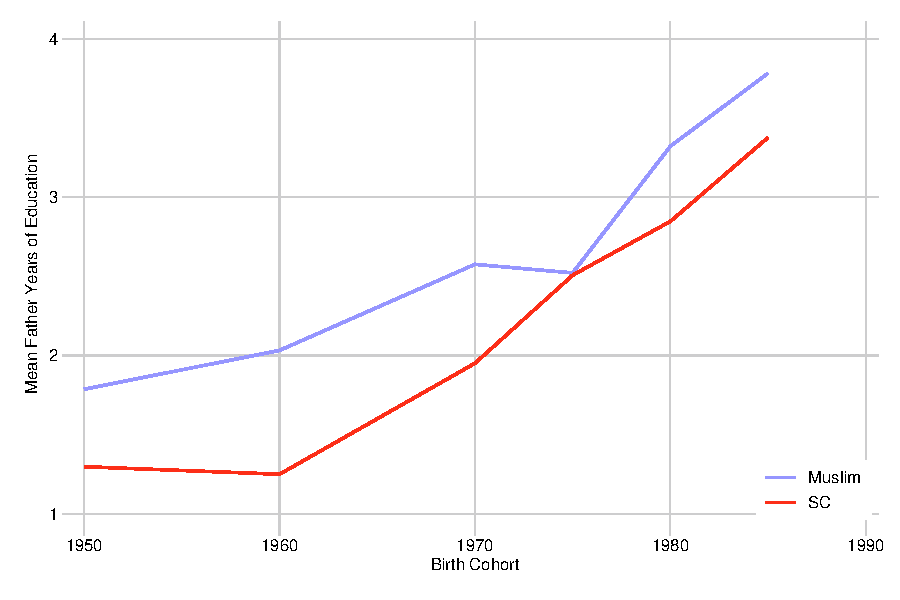
\includegraphics[scale=0.55]{\mobilitypath/sc_mus_father_years} &
      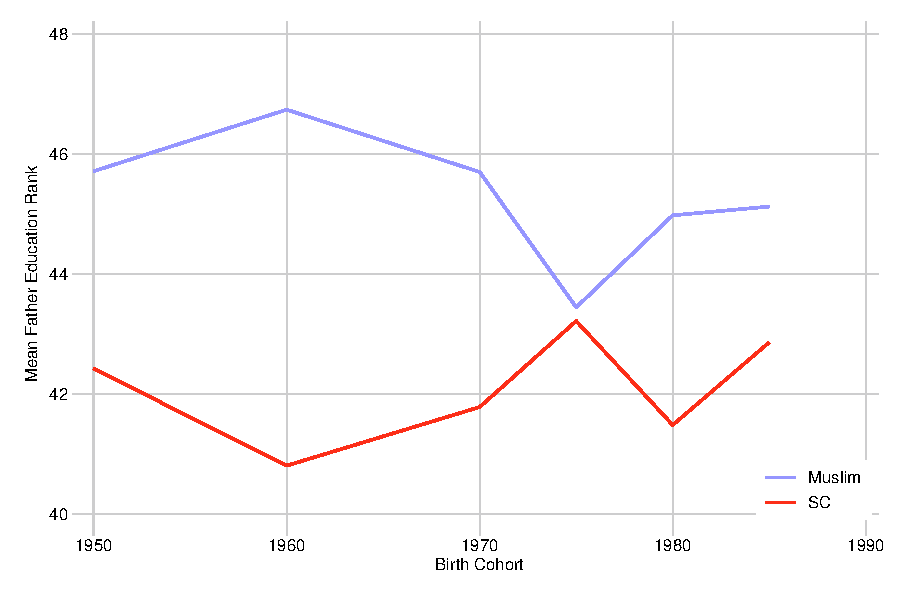
\includegraphics[scale=0.55]{\mobilitypath/sc_mus_father_ranks}
      \\
      
      \panel{C. Log Consumption Gap      vs. Forwards/Others (NSS Households)} &
      \panel{D. Log Consumption Rank Gap vs. Forwards/Others (NSS Households)}    \\ 
      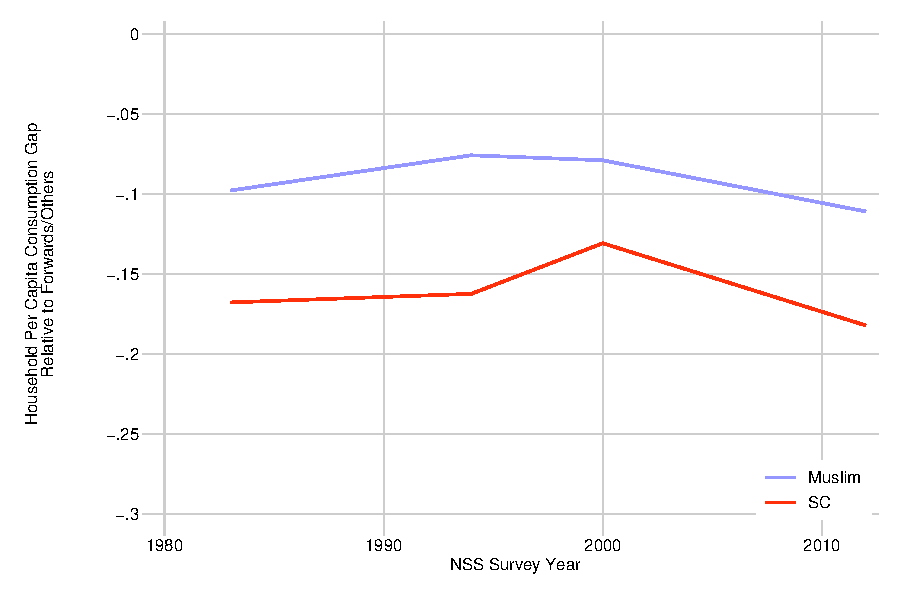
\includegraphics[scale=0.55]{\mobilitypath/mpce_low_line} &
      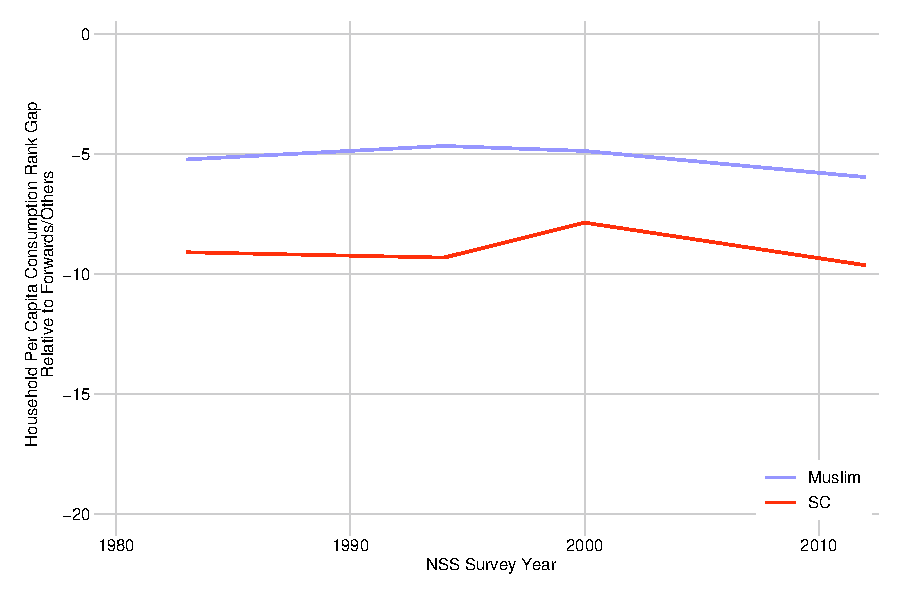
\includegraphics[scale=0.55]{\mobilitypath/mpce_rank_low_line}
      \end{tabular}          
  \end{center}
  \newline
  \footnotesize{\singlespace Figure \ref{fig:sc_muslim_ses_trends} shows trends in socioeconomic status of SCs and Muslims. Panels A and B present education levels (years) and within-cohort education ranks for the \textit{parents} of male respondents in the birth cohorts on the X axis. Ranks are calculated using the midpoint rank of education bins. Panel C uses household-level NSS data to show the log consumption gap between Muslims and Forwards/Others (blue) and SCs and Forwards/Others (red), for households where the head is aged 30--50 and \textit{is in the bottom half of the education distribution.} The X axis shows the NSS survey year. Panel D shows the consumption rank gaps for the same surveys/groups. Source: IHDS (2012), NSS (1983--2012).}
\end{figure}

\clearpage

\subsubsection{Using Within-Subgroup Rank Distributions which are Uniform by Construction}
\label{sec:app_rank_within}

We show here that the Muslim-SC mobility divergence is robust to calculating parent ranks \textit{within} subgroups. Under this rank definition, latent parent ranks within each subgroup are uniform by construction---the latent ranks of SCs in the bottom 50\% of SCs must be uniformly distributed. This fully resolves the non-uniform bias problem, but the cost of making this assumption is that we are no longer comparing groups with similar levels of education---the least educated 50\% of SCs have a lower level of education than the least educated 50\% of Forwards and thus cannot be expected to attain the same outcomes even if there are no cross-group outcome differences after controlling for parent education. For this reason, we use national ranks in the body of the paper. Note that SC and Muslim parents have similar levels of education (much more similar than their children, see Figure~\ref{fig:sc_muslim_ses_trends}), making the latter concern less important here as well.

Figure \ref{fig:subgroup_within_ranks} shows the result. Panel A repeats the result of Figure~\ref{fig:group_mob} for Forwards/Others, Muslims, and SCs, using national ranks, showing changes in upward mobility ($\mu_0^{50}$) over time for each group. Panel B shows the same result, with parent ranks calculated within their own subgroups. The bounds in Panel B are too wide to distinguish mobility changes between SCs and Muslims, because the within-rank bottom-coding problem is more severe among the marginalized groups, where the parent generation is less educated. More than 70\% of SC parents in the 1960s report a bottom-coded education level, resulting in wide bounds on $\mu_0^{50}$ for this rank definition. 

To tighten the bounds, we instead estimate $\mu_0^{70}$: the expected child outcome given a parent in the bottom 70\% of the parent education distribution. Panel C shows $\mu_0^{70}$ calculated using national ranks, as in the body of the paper. Panel D shows $\mu_0^{70}$ calculated using own-subgroup ranks, as in Panel B. The divergence of SCs and Muslims, and the convergence of SCs and Forwards/Others is sustained in both of these panels. The level gap between SCs/Muslims and Forwards/Others is higher in Panels B and D because the bottom $x$\% of SCs/Muslims represent lower levels of education than the bottom $x$\% of Forwards/Others, whereas Panels A and C hold parent education constant.

The consistency of these results with parent ranks calculated within subgroups (which are uniform by construction) strongly suggests that our primary results are not driven by differential unobserved changes in the latent parent rank distributions of the individual subgroups.

%%%%%%%%%%%%%%%%%%%%%%%%%%%%%%%%%%%%%%%%%%%%%%%%%%%%%%%
%% ROBUSTNESS TO ALTERNATE SUBGROUP RANK DEFINITIONS %%
%%%%%%%%%%%%%%%%%%%%%%%%%%%%%%%%%%%%%%%%%%%%%%%%%%%%%%%
\begin{figure}[H]
  \caption{Subgroup Upward Mobility (Fathers/Sons):
    \cnewline National Ranks vs. Within-Subgroup Ranks} 
  \label{fig:subgroup_within_ranks}

  \begin{center}
    \begin{tabular}{cc}
      
      \panel{A. Fathers ranked in national distribution $\mu_0^{50}$} &
      \panel{B. Fathers ranked in subgroup distribution $\mu_0^{50}$}    \\ 
      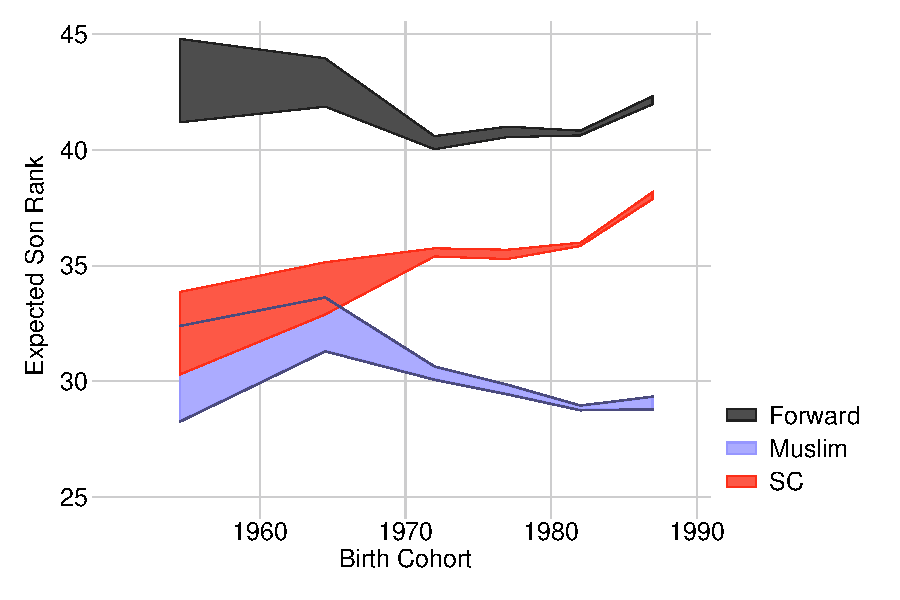
\includegraphics[scale=0.55]{\mobilitypath/ihds_mob_group_across_mu50} &
      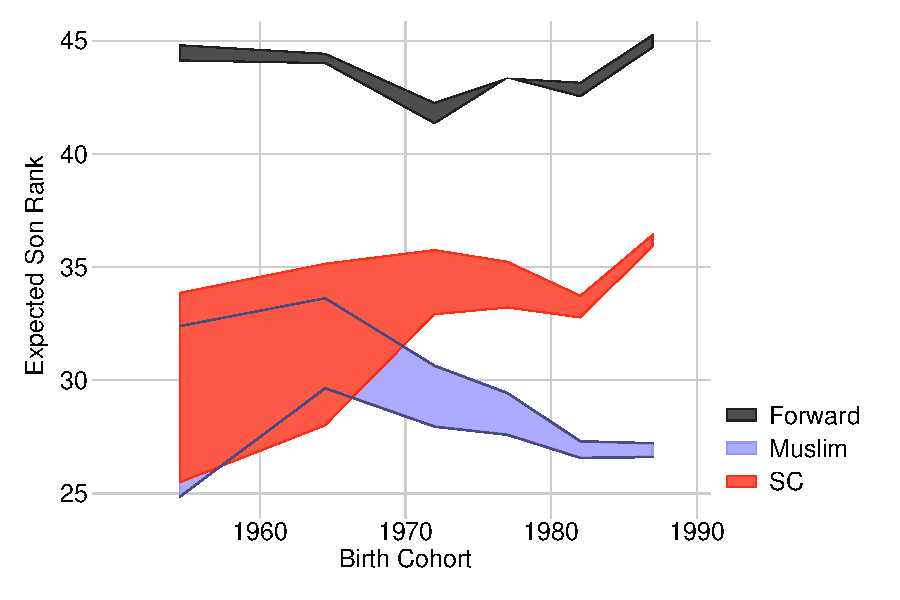
\includegraphics[scale=0.55]{\mobilitypath/ihds_mob_group_within_mu50}
      \\
      
      \panel{C. Fathers ranked in national distribution $\mu_0^{70}$} &
      \panel{D. Fathers ranked in subgroup distribution $\mu_0^{70}$}    \\ 
      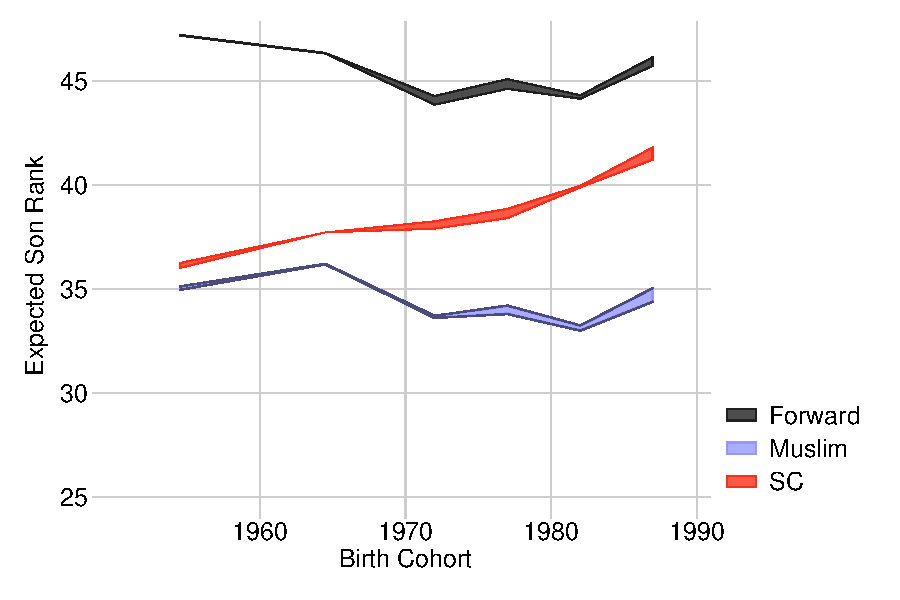
\includegraphics[scale=0.55]{\mobilitypath/ihds_mob_group_across_mu70} &
      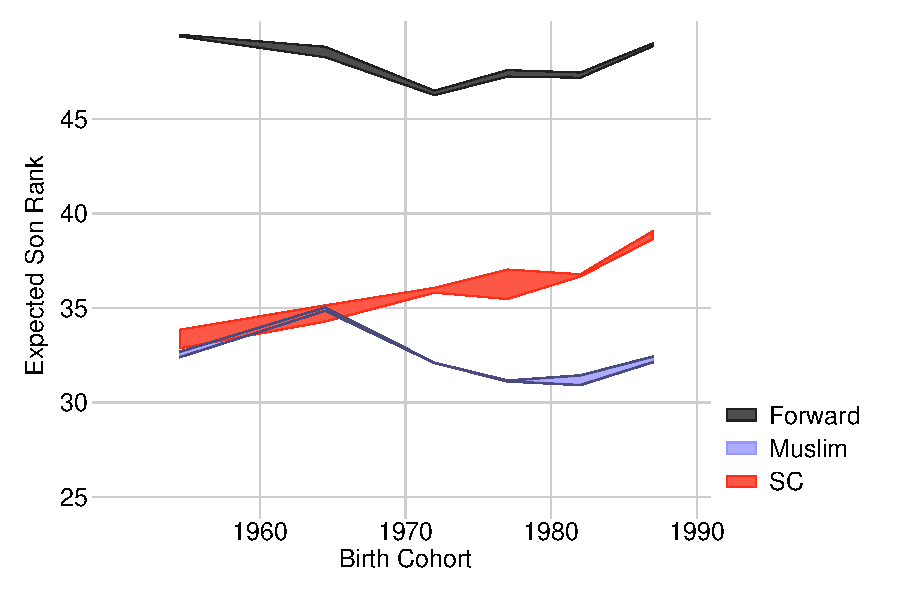
\includegraphics[scale=0.55]{\mobilitypath/ihds_mob_group_within_mu70}
      \end{tabular}          
  \end{center}
  \newline
\footnotesize{\singlespace Figure \ref{fig:subgroup_within_ranks} shows trends in upward mobility for Forward/Others, Muslims, and SCs. Panel A presents bottom-half mobility by ranking fathers in the national distribution, as in the body of the paper. Panel B ranks fathers within each subgroup, recovering uniformity by construction. Panels C and D are similar to A and B, except they present bounds on $\mu_0^{70}$ (i.e., average son rank, conditional on being born to a father in the bottom 70\%) rather than $\mu_0^{50}$. } 
\end{figure}


\subsubsection{Inferring Latent Education Ranks Using Parametric Assumptions}
\label{sec:app_parametric}

This section takes an alternate route to modeling the unobserved variation at the bottom of the education distribution. We assume that the latent rank distribution takes a parametric form (normal or lognormal); we then estimate the full distribution using the cross-bin education distribution for every group.

These parameterized distributions let us produce a continuous latent rank distribution for each subgroup. In the body of the paper, we assumed this distribution was uniform for each group within each bin. The parameterizations let us predict separate within-bin latent rank distributions for each group, based on each group's full distribution of education. We can compare these predicted latent distributions to the uniform distribution used in the paper to gauge the extent of bias that could arise from the uniformity assumption.

For each population subgroup, we fit a normal and a lognormal distribution to the sample distribution of years of education. We then create a simulated population that has the same proportion of each subgroup as the true population, and for each individual, we draw their years of education from the fitted parametric distribution. This gives us a continuous education distribution that matches the moments from the discrete sample distribution.  Finally, we transform the years of education variable into ranks with respect to the entire population. This gives us a simulated population with continuous ranks.

We focus on the 1960--69 and 1985--89 cohorts, as we aim to check the validity of our conclusion that Muslim and SC mobility have diverged over this period.

Table~\ref{tab:sim_moments} compares the moments from the IHDS sample with the moments from the simulated distributions. Here, we are ignoring children and only examining how far the parent latent rank distribution \textit{across groups} differs from what we would get from the uniformity assumption.

For both the 1960--69 and the 1985--89 birth cohorts, the simulated moments are close matches to the raw data. The group ordering and approximate gaps between groups is preserved; the standard deviation of the simulated data is slightly higher than that of the true binned data, which is to be expected, given the truncation of the binned data.

\begin{table}
    \begin{center}
      \caption{Actual and Simulated Moments from the Education Rank Distribution}
      \label{tab:sim_moments}
      \small{
      
\begin{tabular}{rcc|cccc}
\multicolumn{7}{c}{A. 1960-1969 Birth Cohort} \\[0.25ex]
\hline
\hline
& \multicolumn{2}{c|}{\textul{Binned Data}} &  \multicolumn{4}{c}{\textul{Simulated
  Distributions}} \\[0.25ex]
& \multicolumn{2}{c|}{ } &  \multicolumn{2}{c}{Normal} &  \multicolumn{2}{c}{Lognormal} \\[0.25ex]
\hline
& Mean & SD & Mean & SD & Mean & SD \\[0.25ex]
Forward / Other &
55.2 & 26.8 &
55.8 & 30.1 &
55.9 & 29.4 \\[0.25ex]
Muslim &
46.7 & 24.5 &
46.6 & 27.4 &
46.2 & 28.1 \\[0.25ex]
Scheduled Castes &
40.8 & 21.0 &
39.6 & 23.0 &
39.7 & 24.6\\[0.25ex]
Scheduled Tribes &
39.1 & 20.2 &
38.5 & 23.3 &
37.7 & 23.9\\[0.25ex]
\hline
\hline
\\
\\
\multicolumn{7}{c}{B. 1985-1989 Birth Cohort} \\[0.25ex]
\hline
\hline
& \multicolumn{2}{c|}{\textul{Binned Data}} &  \multicolumn{4}{c}{\textul{Simulated
  Distributions}} \\[0.25ex]
& \multicolumn{2}{c|}{ } &  \multicolumn{2}{c}{Normal} &  \multicolumn{2}{c}{Lognormal} \\[0.25ex]
\hline
& Mean & SD & Mean & SD & Mean & SD \\[0.25ex]
Forward / Other &
56.5 & 27.6 &
56.5 & 28.6 &
56.6 & 27.9 \\[0.25ex]
Muslim &
45.1 & 26.7 &
44.8 & 27.5 &
45.4 & 28.2 \\[0.25ex]
Scheduled Castes &
42.9 & 26.7 &
42.8 & 27.5 &
42.6 & 28.1\\[0.25ex]
Scheduled Tribes &
35.6 & 25.0 &
36.1 & 24.9 &
34.9 & 26.1\\[0.25ex]
\hline
\hline
\end{tabular}
}
    \end{center}
Table \ref{tab:sim_moments} shows the mean and standard deviation of the true data (IHDS), compared with the mean and standard deviation of simulated distributions, split by demographic subgroup.
  \end{table}  

In Table~\ref{tab:sim_param_ranks}, we use the simulated data to examine the
distribution of the latent variable \textit{within} the bins where our
method assumed uniformity in the main analysis. Specifically, we examine the mean parent
education rank conditional on being in the bottom 50\%. As expected,
parents from less educated social groups have lower latent ranks even
after conditioning on being in the bottom 50\%.\footnote{If the
  subgroup distributions were all uniform within this bin, then all
  groups would have a mean rank of 25.} However, the
differences are very small, and they do not change much from the
1960--69 to the 1985--89 birth cohorts, under any of the
distributional assumptions. Even in the worst case scenario (the
lognormal distribution with constant variance), the gap between Muslim
and SC parents in the bottom 50\% shrinks from 2.5 to 1, a 1.5
percentage point change.

\begin{table}
  \begin{center}
  \caption{Simulated Average Parent Rank Conditional on Rank $\leq$ 50}
  \label{tab:sim_param_ranks} 
  \small{\begin{tabular}{rcc|cc}
\multicolumn{5}{c}{A. 1960-1969 Birth Cohort} \\[0.25ex]
\hline
\hline
& \multicolumn{2}{c|}{\textul{Group-level Variance}} &  \multicolumn{2}{c}{\textul{Constant Variance}}\\[0.25ex]
& \multicolumn{1}{c}{Normal} & \multicolumn{1}{c|}{Lognormal}  & \multicolumn{1}{c}{Normal}  & \multicolumn{1}{c}{Lognormal}  \\[0.25ex]
\hline
Forward / Other & 24.4 & 25.4 & 27.0 & 27.2 \\[0.25ex]
Muslim & 24.9 & 24.1 & 24.3 & 24.5 \\[0.25ex]
Scheduled Castes & 26.0 & 24.9 & 22.6 & 22.2 \\[0.25ex]
Scheduled Tribes & 25.2 & 24.3 & 21.8 & 21.9 \\[0.25ex]
\hline
\hline
\\
\\
\multicolumn{5}{c}{B. 1985-1989 Birth Cohort} \\[0.25ex]
\hline
\hline
& \multicolumn{2}{c|}{\textul{Group-level Variance}} &  \multicolumn{2}{c}{\textul{Constant Variance}}\\[0.25ex]
& \multicolumn{1}{c}{Normal} & \multicolumn{1}{c|}{Lognormal}  & \multicolumn{1}{c}{Normal}  & \multicolumn{1}{c}{Lognormal}  \\[0.25ex]
\hline
Forward / Other & 26.6 & 27.6 & 27.5 & 27.2 \\[0.25ex]
Muslim & 24.4 & 24.0 & 24.1 & 24.4 \\[0.25ex]
Scheduled Castes & 23.7 & 23.2 & 23.2 & 23.3 \\[0.25ex]
Scheduled Tribes & 22.8 & 21.1 & 21.0 & 21.1 \\[0.25ex]
\hline
\hline
\end{tabular}
}
  \end{center}
Table \ref{tab:sim_param_ranks} presents the simulated average parent rank conditional on being in the bottom half of the distribution under two parametric distributions (normal and lognormal). The left panel estimates distribution mean and variance separately for each demographic subgroup; the right panel uses the same variance for each distribution, estimated from all the data.
\end{table}  

Given the average CEF slope of 0.5, this suggests that changing latent
parental status within the coarse education bins can explain at most
0.75 rank points of the growing difference between Muslims and
SC/STs. Under other distributional assumptions the potential bias is
even smaller. In comparison, our midpoint estimate of this change from
1960--69 to 1985--89 in the body of the paper is 7.4 rank points. This is not a strict upper bound, because child outcomes could be correlated with latent ranks, something we do not address here. But the scale of the effect on the average rank difference conditional on being in the bottom half strongly suggests that non-uniformity within bins is not a major factor explaining our results.

In short, we consider it unlikely that changing parental position
within observed rank bins can explain the growing mobility gap between
SCs and Muslims. All the evidence brought to bear suggests that the relative positions of these groups within the bottom education
bins has not changed enough to substantially bias our
group-level estimates.

% \subsection{Robustness to Adjusting for Censored Child Ranks}
% \label{sec:app_child_censoring}
% 
% In the main part of the paper, we focus on bounding a function $Y(x) =
% E(y|x)$ when $y$ is observed without error, but $x$ is observed with
% interval censoring. In this section, we modify the setup to consider
% simultaneous interval censoring in the conditioning variable $x$ and
% in observed outcomes $y$. In the mobility context, this
% double-censoring setup arises when the $y$ variable is a child rank
% (as in Figure~\ref{fig:mu_gender}A and \ref{fig:mu_gender}B), but not
% when the $y$ variable is a child level of education (as in
% Figure~\ref{fig:mu_gender}C and \ref{fig:mu_gender}D). As noted in the
% paper, all of our results are consistent whether we use levels or
% ranks as outcomes. We nevertheless proceed here to examine the
% potential bias from ignoring the censoring of child ranks.
% 
% One approach to this problem would be to use a problem setup similar
% to that presented in Section~\ref{sec:method}, that takes into account
% the information on child ranks that is lost by binning. We developed a
% numerical optimization that could bound the CEF by searching over all
% possible joint distributions of latent $x$ and $y$ variables, but with
% $n^2$ the number of parameters compared with the single-censoring
% model, it proved computationally infeasible.
% 
% We therefore present two alternate approaches to the problem here.
% First, we define the latent distributions of $y$ variables that would
% generate the maximal and minimal mobility statistic in theory. We can
% then bound the mobility statistic following our standard method under
% these best- and worst-case assumptions. This union of these bounds is
% a very conservative bound on the mobility statistic given censoring in
% both the $y$ and $x$ variables.
% 
% Second, we can shed light on the distribution of the true average
% value of $y$ in each $x$ bin if other data is available. This approach
% is feasible whenever more information is available about children than
% about their parents, as is the case in our context (and in many
% others).  Specifically, we use data on child wages to predict whether
% the true latent child rank distribution ($y$) is better represented by
% the best- or worst-case mobility scenario. The joint wage distribution
% suggests that the true latent distribution of $y$ in each bin is very
% close to the best case distribution, which we used in
% Section~\ref{sec:results}.
% 
% % , because there is little effect of parent
% % education on child wages after conditioning on child education.
% 
% \subsubsection{Best and Worst Case Mobility Distributions}
% \label{sec:best_worst}
% 
% In this section, we take a sequential approach to the double-censoring
% problem. We first calculate the set of child CDFs for each level of
% parent education that would correspond to the highest and lowest
% possible intergenerational mobility. From these CDFs, we can calculate
% the average latent rank of children in each parent bin. These may be
% different from the latent rank implied by assigning each child the
% midpoint of their bin. With these latent ranks, we can then follow the
% estimation procedure outlined in Section~\ref{sec:method}. This gets
% us a wider set of bounds that takes the censoring of child ranks into
% account.
% 
% To make the example concrete, consider two children who have less than
% 2 years of education; one is from a rich family and one is from a poor
% family. Assume that 20\% of children in the population have less than
% 2 years of education. In the body of the paper, we would assume that
% each of these children has a rank of 10 (i.e. the midpoint of the
% bottom bin). But it is possible that the child from a poor family has
% a latent rank of 7 and the child from a rich family has a latent rank
% of 13. In this case, mobility would be lower than what we have
% measured in the paper.
% 
% Given that child rank is known only to lie in one of $h$ bins,
% there are two hypothetical scenarios that describe the best and worst
% cases of intergenerational mobility. Mobility will be lowest if child
% outcomes are sorted perfectly according to parent outcomes
% \textit{within} each child bin, and highest if there is no additional
% sorting within bins.\footnote{Specifically, these scenarios
%   respectively minimize and maximize both the rank-rank gradient and
%   $\mu_0^{x}$ for any value of $x$. To minimize and maximize $p_x$, a different
%   within-bin arrangement is required for every $x$. We leave this out
%   for the sake of brevity, and because bounds on $p_x$ are minimally
%   informative even with uncensored $y$.}
% 
% Note that the case of perfect sorting within bins fits very poorly
% with the standard human capital model. In this model, the binned
% education data reflects a continuous demand for education with a lumpy
% number of years available for purchase. It is difficult to theorize a
% distribution where there is a large mass of rich children bunched just
% below a bin boundary, and no rich children just above that boundary.
% Given that children of rich and poor parents appear in every bin in
% the child distribution, the true distribution is likely to be closer
% to the uniform case than the perfectly ordered case.  Note also that
% we do not consider the case of perfectly reversed sorting, where the
% children of the least educated parents occupy the highest ranks within
% each child rank bin, as it would violate the stochastic dominance
% condition (and is implausible).
% 
% Appendix Figure~\ref{fig:son_solution} shows two set of CDFs that
% correspond to these two scenarios for the 1960--69 birth cohort.  In
% Panel A, children's ranks are perfectly sorted according to parent
% education within bins. Each line shows the CDF of child rank, given
% some father education. The points on the graph correspond to the
% observations in the data---the value of each CDF is known at each of
% these points and thus the CDFs must pass through them.  Children below
% the 27th percentile are in the lowest observed education bin. Within
% this bin, the CDF for children with the least educated parents is
% concave, and the CDF for children with the most educated parents is
% convex---indicating that children from the best off families have the
% highest ranks within this bin. This pattern is repeated within each
% child bin.  The implausibility of this scenario is reflected by the
% kinked nature of these CDFs, which are unlikely to appear in the real
% world. Panel B presents the high mobility scenario, where children's
% outcomes are uniformly distributed within child education bins, and
% are independent of parent education within child bin.
% 
% Each of these CDFs can be collapsed to a single mean child rank for
% each parent bin. From these expected child ranks, we can then use the
% method from Section~\ref{sec:method} to calculate bounds on any
% mobility statistic. The top two rows of Table~\ref{tab:double_censor}
% shows bounds on $\mu_0^{50}$ and on the rank-rank gradient for the
% high and low mobility scenarios.  Taking censoring in the child
% distribution into account widens the bounds on all parameters. The
% effect is proportionally larger for bottom half mobility, because it
% was so precisely estimated before---the bounds on $\mu_0^{50}$
% approximately double in width when censoring of son data is taken into
% account.
% 
% These bounds are very conservative, as the worst case scenario is
% implausible, as noted above. In the next subsection, we draw on
% additional data on children, which suggests that the best case
% mobility scenario is close to the true joint latent distribution.
% 
% \subsubsection{Estimating the Child Distribution Within Censored Bins}
% 
% Because we have additional data on children, we can estimate the shape
% of the child CDF within parent-child education bins using rank data
% from other outcome variables that are not censored. Under the
% assumption that latent education rank is correlated with other
% measures of socioeconomic rank, this exercise sheds light on whether
% Panel A or Panel B in Figure~\ref{fig:son_solution} better describes
% the true latent distribution.
% 
% Figure~\ref{fig:son_wage_cdf} shows the result of this exercise using wage data
% from men in the 1960s birth cohort. To generate this figure, we
% calculate children's ranks first according to education, and then
% according to wage ranks within each education bin.\footnote{We limit
%   the sample to the ~50\% of men who report wages. Results are similar
%   if we use household income, which is available for all
%   men. Household income has few missing observations, but in the many
%   households where fathers are coresident with their sons, it is
%   impossible to isolate the son's contribution to household income
%   from the father's, which biases mobility estimates downward.} The
% solid lines depict this uncensored rank distribution for each father
% education; the dashed gray lines overlay the estimates from the high
% mobility scenario in Panel B of Figure~\ref{fig:son_solution}.
% 
% If parent education strongly predicted child wages \textit{within}
% each child education bin, we would see a graph like Panel A of
% Figure~\ref{fig:son_solution}. The data clearly reject this
% hypothesis. There is some additional curvature in the expected
% direction in some bins, particularly among the small set of
% college-educated children, but the distribution of child cumulative
% distribution functions is strikingly close to the high mobility
% scenario, where father education has only a small effect on
% child wage ranks after child education is taken into account. The last
% row of Table~\ref{tab:double_censor} shows mobility estimates using
% the within-bin parent-child distributions that are predicted by child
% wages; the mobility estimates are nearly identical to the high
% mobility scenario. This result suggests that our assumption in
% Section~\ref{sec:results} that the latent child rank is the midpoint of
% the rank bin for all parent groups is not affecting our estimates very
% much.
% 
% Note that there is no comparable exercise that we can conduct to
% improve upon the situation when parent ranks are interval censored,
% because we have no information on parents other than their education,
% as is common in mobility studies. 
% 
% Note finally that the potential bias from assuming uniformity within
% child rank bins is increasing in the size of the rank bins. Because
% children are more educated than parents in every cohort, this bias is
% smaller for children than it would be for parents. It is also smaller
% for the younger cohorts of children born in the 1980s than it is for
% the example we used here.
% 
% %%%%%%%%%%%%%%%%%%%%%%%%%%%%%%
% %% BEGIN APPENDIX C FIGURES %%
% %%%%%%%%%%%%%%%%%%%%%%%%%%%%%%
% {\singlespacing
% \begin{figure}[H]
% 
%   \caption{Best- and Worst-Case Son CDFs \cnewline by Father Education (1960-69
%     Birth Cohort)}
%   \label{fig:son_solution}
% 
%   \begin{center}
%     \begin{tabular}{c}
% 
%       Panel A: Lowest Feasible Mobility
%       \\
%       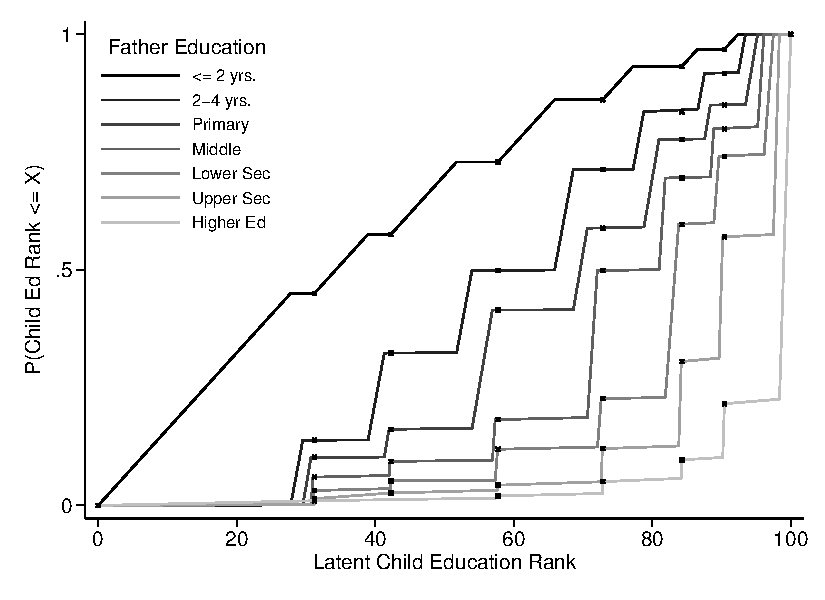
\includegraphics[scale=0.80]{\mobilitypath/cdf_low_mob} \\
%       \\
%       \\
%       Panel B: Highest Feasible Mobility
%       \\
%       \includegraphics[scale=0.80]{\mobilitypath/cdf_high_mob} \\
% 
%     \end{tabular}
%     \hline
%   \end{center}
% 
%   { \footnotesize Figure~\ref{fig:son_solution} shows a set child CDFs
%     conditional on each level of father education that correspond to
%     the best and worst case scenarios for intergenerational
%     mobility. The lines index father types. Each point on a line shows
%     the probability that a child of a given father type obtains an
%     education rank less than or equal to the value on the X axis in
%     the national education distribution. The large markers show the
%     points observed in the data.}
% 
% \end{figure}
% 
% \begin{figure}[H]
%   \caption{Son Outcome Rank CDF \cnewline
%     by Father Education (1960-69 Birth
%     Cohort) \cnewline {\small Joint Education/Wage Estimates}} 
%   \label{fig:son_wage_cdf}
%   \begin{center}
%     \includegraphics[scale=0.80]{\mobilitypath/cdf_combined}
%     \hline
%   \end{center}
%       {\small Figure~\ref{fig:son_wage_cdf} plots a son rank
%         CDF separately for each father
%         education level, for sons born in the 1960s in India. Sons
%         are ranked first in terms of education, and then in terms of
%         wages. Sons not reporting
%         wages are dropped. For each father type, the graph shows a
%         child's probability of attaining less than or equal to the
%         rank given on the X axis.}
% \end{figure}
% 
% \floatbarrier
% 
% \begin{table}[H]
%   \caption{Mobility Estimates under Double-Censored CEF }
%   \label{tab:double_censor} 
%   \begin{tabular}{lcc}
\hline\hline
  &  Upward Interval          &  Rank-Rank \\
  & Mobility ($\mu_0^{50}$)  &  Gradient ($\beta$)        \\
Low mobility scenario &   [32.33, 35.90]          &  [0.55, 0.80]  \\
High mobility scenario &  [35.86, 38.80]      &  [0.45, 0.67]  \\
Wage imputation scenario &  [35.79, 38.70]     &  [0.46, 0.67]  \\

\hline
\end{tabular}


% \end{table}  
% \footnotesize{Table \ref{tab:double_censor} presents bounds on
%   $\mu_0^{50}$ and the rank-rank gradient $\beta$ under
%   three different sets of assumptions about child rank distribution
%   within child rank bins. The low mobility scenario assumes children
%   are ranked by parent education within child bins. The high mobility
%   scenario assumes parent rank does not affect child rank after
%   conditioning on child education bin. The wage imputation predicts the
%   within-bin child rank distribution using child wage ranks and parent
%   education.}
% 
% }


  \newpage
  \floatbarrier
  
  \section{Appendix D: Data Construction}
  \label{app:data}
  
This section describes the data sources and data construction in
detail. 

\subsection{IHDS}

The India Human Development Survey (IHDS) is a nationally
representative survey of 41,554 households, with rounds in 2004--05
and 2011--12. Definitions of social groups are described in the body
of the paper. This section focuses on linking parents to children.

The primary module of IHDS records the education of the father of the household
head. A secondary module, the women's survey, records the education of
the father and mother of the female respondent, as well as the father
and mother of her husband if she is married. The women's survey is
given to one or two women aged 15--49 in each household. Because of
the upper age restriction on the women's survey, the oldest daughter
in our sample is born in 1962; we therefore do not have any links from
mothers or links to daughters for the 1950--59 birth cohort.

Finally, we created additional parent-child links using information
from the relationship field in the household roster. Specifically, we
linked the household head to their children and parents. We linked the
spouse of the household head to their children. We linked
grandchildren of the household head to the child of the household only
in cases where there was no possible ambiguity about the parents of
the grandchildren. In cases with no possible ambiguity, we linked
nieces/nephews of the household head to brothers of the household
head. We did not link individuals on the basis of in-law
relationships, because of the ambiguity in the definition of the
sibling-in-law (i.e. sibling of spouse vs. spouse of sibling).

In many cases, a parent's education is recorded in multiple ways,
allowing us to cross-check the validity of the responses.  For
example, the household head's father's education may be obtained from
(i) the household roster (if he is coresident); (ii) from the
household head's response to the father education question; and (iii)
from his wife's responses to the husband's father's education
question. The average correlation between parent education measured
across different sources is 0.9. Appendix Table~\ref{tab:validate_eds}
shows that the discrepancies between measures are not correlated with
household characteristics.

\subsection{Data from other countries}

We refer in the paper to mobility data from several other
countries. Data from Denmark, Sweden, and Norway were generously
shared with us by \citeasnoun{boserup2014} and
\citeasnoun{bratberg2017}. Income mobility estimates for the U.S. were
drawn from \citeasnoun{chetty2014b} and
\citeasnoun{chetty2018}. Educational mobility estimates from the
U.S. were calculated from a parent-child education transition matrix
describing children in the 2005--2015 ACS and parents in the 2000
Census, from the data package of \citeasnoun{chetty2018}.


}
\end{appendix}

\end{document}

